\documentclass[a4paper,12pt]{article}
\usepackage[margin=0.7in]{geometry}
\usepackage[latin1]{inputenc}
\usepackage[english]{babel}
\usepackage{amsmath}
\usepackage{cases}
\usepackage[makeroom]{cancel}
\usepackage{amsmath,tabu}
\usepackage[fleqn]{mathtools}
\usepackage[fleqn]{amsmath}
\usepackage{bm}
\usepackage{tikz}
\usepackage{enumitem}
\usepackage{wrapfig}
\usepackage{graphicx}
\usepackage{siunitx}
\usepackage{microtype}
\usepackage{array,tabularx}
\usepackage{float}
\usepackage{booktabs}
\usepackage{import}
\usepackage{cases}
\usepackage{graphicx,subfigure}
\usepackage{myUnitOfMeasure}
%\usepackage{myThermodynamics}
\usepackage{myMath}
\usepackage{mathtools}
\usepackage{gensymb}
\usepackage{xcolor}
\usepackage{url}
\usepackage{tabularx}
\usepackage{ltablex}
\usepackage{booktabs}
\usepackage{float}
\usepackage{listings}
\restylefloat{table} % with H force table position

\title{
\includegraphics[scale=0.4]{images/logo.png}
\\[1cm]
FINAL REPORT - THE MRL TURBINE SIMULATION
\\
MODELING TECHNIQUES FOR FLUID MACHINES 
\\
A.Y. 2017/2018}
\author{
Andrea Rossi \and Marco Bonasegale
\and Marco Belloli \and Alberto Casali
%\includegraphics[width=\textwidth]{images/cover.png}
}
\date{}

% usefull for ltablex to split long tables in many pages
\keepXColumns

\DeclarePairedDelimiter\abs{\lvert}{\rvert}%

%\newcommand{\Fy}[1]{\text{F}_{y_{#1}}}

%\newcommand{\diameter}{\oslash}

%\newcommand{\todo}{\colorbox{cyan!60}{TODO}}

\renewcommand{\thesubsection}{\thesection.\arabic{subsection}}

\renewcommand{\arraystretch}{1.4}

\newcommand{\variable}[1]{\textcolor{blue}{#1}}

\newcommand{\paramtext}[1]{\textcolor{black!30!green}{#1}}

\newcommand{\terminal}[1]{\textcolor{black!30!cyan}{#1}}

\newcommand{\todo}{\colorbox{cyan!60}{TODO}}

\newcommand{\nut}{\nu_\text{T}}

\newcommand{\foam}[1]{{\ttfamily #1}}

\newcommand{\kepsilon}{$k\!-\!\varepsilon $ } 

\newcommand{\komegasst}{$k\!-\!\omega \, \text{SST} $ } 



\lstset{
	basicstyle=\fontsize{11}{13}\selectfont\ttfamily,
    frame=tb, % draw a frame at the top and bottom of the code block
    tabsize=4, % tab space width
    showstringspaces=false, % don't mark spaces in strings
    numbers=left, % display line numbers on the left
    commentstyle=\color{black!50!green}, % comment color
    keywordstyle=\color{blue!50!cyan}, % keyword color
    stringstyle=\color{black!30!red} % string color
}



\newcommand{\fakecaption}{%
  \vskip0.5\baselineskip
  \refstepcounter{table}%
  \tablename\ \thetable%
}

\makeindex

\begin{document}

\maketitle
\begin{center}
\includegraphics[width=\textwidth]{images/cover.png}
\end{center}

\newpage

\tableofcontents

\newpage

\section{Introduction}

\subsection{MRL Tidal Turbine Description}
The MRL Turbine is a hydraulic machine which is able to exploit the upcoming  water flow that is passing through the cross sectional area of the inlet of the machine. Momentum Reversal and Lift Tidal Turbine is a cross-flow tidal-stream device which converts the energy of the water
flow into mechanical power. So the most advantageous locations in order to place this device are whatever kind of regular river with a smooth river bed or any sea/ocean areas which are subjected to relevant tidal phenomena.
The turbine is made up of three rotating blades and each blade is subjected to the combination of two rotating motions. A rotation $\omega_0$ along the machine axis  and a rotation $\omega_1$ around the blade individual axis with counter-rotating $\omega_0$ and $\omega_1$.

\begin{center}
\includegraphics[width=0.8\textwidth]{images/flow.png} 
\end{center}

The flow-blade interaction leads to a drag force that is coming out while the blade is placed in the upper part of the circumferential path and a lift force on each blade located in the lower part of the path.
The resulting torque multiplied by the rotating speed will give the generated power of the turbine which, in the end, is our final useful effect. The generated power per turbine is not really high (a few Watts) and this is the reason why the \emph{farm layout}  that Prof. Gavin Tabor showed us at the beginning of the course is used. Many little turbines are placed in a schematic and regular disposition in order to extract a higher power from the tidal stream.
Since from the first raw presentation of the machine we can realise that the mesh will have a relevant importance in the representation and validation of this complex rotating movement. We will deal with a rotating mesh which is progressivly refined close to the blades, ending with the boundary layers when we are approaching the solid walls of the blades.


\subsection{The data}
The turbine is surrounded by an upcoming water flow set at 1 m/s constant along y axis. 
CAD files were provided by our professor and all the geometry parameters were known.
The in-class workflow has been divided into four little sub-tasks. 

The sub-tasks allowed us to start to get more familiar with the project work and understand the main issues met along the path with the help of the professors.

\section{In-class work}
\paragraph{In-class workflow}\mbox{}\\
 The in-class project started with the raw mesh generation (blockMesh, snappyHexMesh), continued with the preparation of the rotating mesh(AMI files, baffles creation, merge and split procedure), movement of the mesh with the provided motion laws  (real turbine rotation, gif rendering) and finally the set up, running and post processing of the simulation.

\subsection{Mesh generation}\mbox{}\\
One of the most challenging section of the in-class project was the generation of the raw turbine domain mesh. We have used many different openFoam comands in order to build a complete and exhaustive mesh that must be suitable for the hydraulic problem characteristics.
\\ 
Let's start to present the overall mesh work-flow with all the brief steps evaluation.
\\
\begin{itemize}
\item The scaling of the dimensions and geometry parameters coming from the stl files from millimiters to meters in order to perform correct calculations in the openFoam environment;

\item BlockMesh and SnappyHexMesh for each of the three blades. At this point castellated, snapped and layered mesh have been realized for each blade and we have to join all together;

\item Merging procedure in order to have one complete mesh and the copy of the mesh inside our main environment of the project. We have decided to oparate in this way in order to have a better comunication level in terms of interpolation values among mesh sub-domains. In this way the neighboring cells of different sub-domains are well oriented and aligned. The result is an improvement on the mesh quality controls as non-orthogonality index and skewness coefficient  because we have parallel disposition of cells and they appear as concentric refined layers;

\item Mesh extrusion with the thickness of the 2D domain already given as a geometry parameter equal to the blade width;

\item Wall layer refinement;

\item The first mesh is the 40$\times$120 mesh where the couple of numbers indicates the number of squared and regular cells that are disposed in the y and x direction respectively in the blockMeshDict definition.  
\end{itemize}

Since we deal quite often with different mesh size, in particular during the mesh senitivity analysis, we will call mesh $i$ the mesh with $i$ cells in the y direction, and the cells in the x direction are such a number that let to have squared cells, in order to make the comparison easier and faster to understand.


\subsection{Boundary conditions}\mbox{}\\

Boundary conditions are referred to the water stream velocity that is investing the machine, the pressure of the water in the stream channel, $k$ , $\omega$ and $\nu_T$ values.

Our main interest is to focus onto the first two boundary conditions so velocity and pressure, since the other are mainly taken as default conditions for the respective turbolence model.

\paragraph{Patches}\mbox{}\\
Boundary condition are defied over patches so it is important to define that.
\begin{itemize}
\item \emph{Inlet Section} is that from which water comes into the domain moving towards the x direction;
\item \emph{Outlet Section} is where water comes out from the domain;
\item \emph{Front and back faces} are always set to empty since we are dealing with a 2D problem;
\item \emph{Lower wall} is a physical wall that limit the flow (think about river bed!);
\item \emph{Upper wall} is a free surface where the flow can slip;
\item \emph{Blades} are physical surfaces that moves inside the domain;
\item \emph{Ami interfaces} are internal patches that allow the communication between moving adiacent cells. All the quantities are set as CyclicAmi.
\end{itemize}


\paragraph{Velocity U}
\begin{itemize}
\item \textbf{Internal field} is uniform at the beginning and it is set to $1\ms$ in the x direction even if in class we have set inlet velocity to $1\ms$ and internal field uniformly set to $0\ms$. We take this decision to make the transition phase faster to limit the simulation time. We are actually interested only in staeady state power so limiting the transition let us to reduce computational time;
\item \emph{Inlet Section} velocity is fixed to $1\ms$ during all the simulation; 
\item \emph{Outlet Section} velocity is unknown so we have to set it to ZeroGradient boundary condition;
\item \emph{Upper wall} velocity is set to Slip since the fluid can flow in the free stream;
\item \emph{Lower wall} velocity is set to NoSlip which is equivalent to fix the value to zero;
\item \emph{Blades} velocity is set to MovingWallVelocity which is equivalent to NoSlip for moving bodies;
\end{itemize}

\paragraph{Pressure $p$}
\begin{itemize}
\item \textbf{Internal field} is uniform at the beginning and it is set to $0$. 
OpenFoam for incompressible cases works with pressure normalized respect to density. 
Moreover it can manage relative pressures. 
So the value that we set is relative $0 \,\text{bar} \cdot \text{m}^3 / \kg = \m / \s^2$.
\item \emph{Inlet Section} pressure distribution unknown so we set to ZeroGradient; 
\item \emph{Outlet Section} is set to atmospheric ($0 \m / \s^2$) since we assume to be sufficiently far from the blades so that pressure can be evalueted constant;
\item \emph{Upper wall} pressure is set to atmospheric since it is free stream;
\item \emph{Lower wall} pressure is set to ZeroGradient since boundary layer are isobar;
\item \emph{Blades} pressure is set to ZeroGradient since boundary layer are isobar;
\end{itemize}

\paragraph{Turbolent quantities $k$, $\varepsilon$, $\omega$, $\nu_T$}\mbox{}\\
For what that concern the boundary conditions of the turbolence quantities we apply default settings.
We will discuss instead a modification of the value of initialization of that quantities to speed up as much as possible the convergence to a steady state condition.

\paragraph{Solver}\mbox{}\\
The solver applied in the class session is pimpleDyMFoam in PISO mode with one outer corrector, two inner correctors and no non orthogonal correctors. This solver is responsible not only for the solution of the system of differential equation, but also for the movement of the mesh at each time step. 

\subsection{In-class results}\mbox{}\\
In the final part of the in-class project we performed the set up and run of the first raw simulation.
To do so, we have to manage with the boundary conditions of the problem, the turbolence modeling and the numeric schemes. All these macro-section of the simulation were assigned a priori and the last part of our work is to play with all these parameters and try to understand the influence of each singular changing in the set up on the final result that the turbine must provide.

For the first setup we use the simpler $k\!-\!\varepsilon$ turbolence model respect to a more appropriate $k\!-\!\omega \, \text{SST}$.

Analysing $y^+$ from table \ref{table:inclass-yplus} we can notice that even with a quite coarse mesh we have $y^+$ much smaller that 30 which is the
minimum threshold under which $k\!-\!\varepsilon$ is not suitable; this is the reason why in the next part of this report we will always adopt $k\!-\!\omega \, \text{SST}$ except when differently specified.
\begin{table}[H]
\centering
\begin{tabular}{lrrr}
\toprule
$y^+$     & Minimum             & Maximum            & Average            \\ \midrule
lowerWall & $\round{11.58443}$  & $\round{18.03507}$ & $\round{14.0232}$  \\
blade0    & $\round{0.7735179}$ & $\round{9.497755}$ & $\round{4.377209}$ \\
blade1    & $\round{1.072712}$  & $\round{3.972875}$ & $\round{2.488902}$ \\
blade2    & $\round{0.4794929}$ & $\round{9.077512}$ & $\round{5.569296}$ \\ \bottomrule
\end{tabular}
\caption{$y^+$ at time 2.4 seconds}
\label{table:inclass-yplus}
\end{table}

The final results of the first raw simulation are provided in following figure.

\begin{figure}[H]
\subfigure[Pressure at 2.4]{\includegraphics[width=8.5cm]{images/inclass/{pfield2.4sec}.png}}
\hfill
\subfigure[Velocity at 2.4]{\includegraphics[width=8.5cm]{images/inclass/{velocityfield2.4sec}.png}}
\caption{In class work results.}
\end{figure}

\begin{figure}[H]
\centering
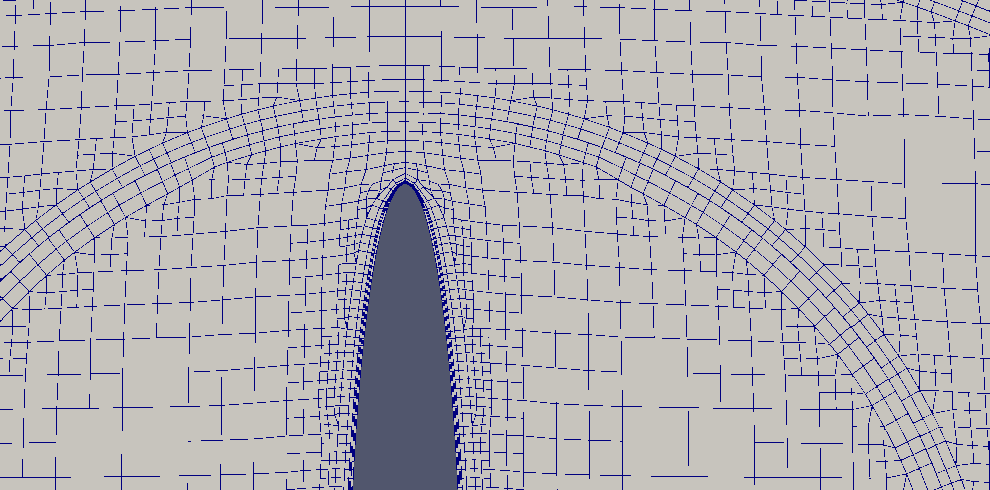
\includegraphics[width=14cm]{images/inclass/mesh40.pdf}
\end{figure}

In table \ref{table:inclass-power} we have reported the mean power computed in the last round, between 1.8 and 2.4 seconds.
This choice derives from the analysis of the trend of the instantaneous power plotted in figure \ref{fig:inclass-instantpower}
that shows that the power reaches steadyness condition after 3 complete revolutions.

\begin{table}[H]
\centering
\begin{tabular}{lr}
\toprule
Power (Pressure) [W]     & $\round{4.84602561871}$   \\ \midrule
Power (Shear stress) (W) & $\round{-0.253811271949}$ \\
Power (Total) [W]        & $\round{4.59221434676}$   \\ \bottomrule
\end{tabular}
\caption{Mean power between 1.8 and 2.4}
\label{table:inclass-power}
\end{table}

\begin{figure}[H]
\centering
\includegraphics[width=14cm]{images/inclass/instantpower.png}
\caption{Instant power}
\label{fig:inclass-instantpower}
\end{figure}


\section{Mesh sensitivity Analysis}
With the mesh sensitivity analysis second part of the report starts. Here we are interested to find the proper value of parameters that let to have the best simulation as possible.

The first and probably the most significant operation is the mesh sensitivity analysis.
\\
The aim is to find a tradeoff between \emph{accuracy} and \emph{computational cost}. 

The expected improvement into the quantities of interest decreases with the increase of the number of cells.

There is a point beyond which the improvement becomes really negligible and we encounter a plateau; beyond that it does not worth the increase in computational time. 

Our sensitivity analysis includes 6 different simulations:
\begin{itemize}
\item mesh 20
\item mesh 40
\item mesh 60
\item mesh 80
\item mesh 120
\item mesh 160
\end{itemize}

The choise of the level of vertical cells depends on the need to exploit 3 different steps in which the number of cells becomes 4 times bigger. Actually we pass from approximately 10000 cells of the mesh 20 to 40000 cells of the mesh 80 finally to around 160000 cells of the mesh 160. 
The ratio four explains the necessity to double the cells number in each of the relevant dimensions of our 2D problem.

Despite the fact that the power generated is not the best indicator possible for highliting sensitivity behaviour it is instead the most relevant output parameter of our simulation.
Beside that we put also the total pressure drop that is a measure of the losses due to the turbine.
To compute the drop we consider the average of the total pressure at the inlet and at the outlet both calculated at the end of the simulation.

During the choice of the mesh we have exploited two different possibilities:
\begin{itemize}
\item with a refinement region around the blades;
\item without a refinement region.
\end{itemize}
In both cases the same layer were present.
What we have noticed is that the results in terms of power were slighlty different, so we have decided to perform mesh sensitivity analysis with both the meshes.

\begin{figure}
\subfigure[Mesh 120 without refinement region]{\includegraphics[width=8.5cm]{images/meshsensitivity/mesh120-blade0-noregion.png}}
\hfill
\subfigure[Mesh 120 with refinement region]{\includegraphics[width=8.5cm]{images/meshsensitivity/mesh120-blade0-region.png}}
\caption{Comparison between meshes with and without refinement.}
\end{figure}

\begin{figure}
\subfigure[Mesh 20 without refinement region]{\includegraphics[width=8.5cm]{images/meshsensitivity/mesh20-blade0-noregion.png}}
\hfill
\subfigure[Mesh 40 without refinement region]{\includegraphics[width=8.5cm]{images/meshsensitivity/mesh40-blade0-noregion.png}}
\subfigure[Mesh 60 without refinement region]{\includegraphics[width=8.5cm]{images/meshsensitivity/mesh60-blade0-noregion.png}}
\hfill
\subfigure[Mesh 80 without refinement region]{\includegraphics[width=8.5cm]{images/meshsensitivity/mesh80-blade0-noregion.png}}
\subfigure[Mesh 120 without refinement region]{\includegraphics[width=8.5cm]{images/meshsensitivity/mesh120-blade0-noregion.png}}
\hfill
\subfigure[Mesh 160 without refinement region]{\includegraphics[width=8.5cm]{images/meshsensitivity/mesh160-blade0-noregion.png}}
\caption{Comparison between different mesh sizes.}
\label{fig:noregion-allmeshes}
\end{figure}

Given the mesh in figure \ref{fig:noregion-allmeshes} we have performed the simulation and extracted both power and total pressure drop.

\paragraph{Number of cells}\mbox{}\\
In table \ref{table:cellsnumber} we can find the cells number of the various simulations.
\begin{table}[H]
\centering
%\begin{tabular}{@{}lrr@{}}
\begin{tabular}{lrr}
\toprule
         & Without region & With region \\ \midrule
Mesh 20  & 10328          & 9696        \\
Mesh 40  & 24066          & 24021       \\
Mesh 60  & 40462          & 42508       \\
Mesh 80  & 58877          & 64293       \\
Mesh 120 & 103384         & 120614      \\
Mesh 160 & 156791         & 160547      \\ \bottomrule
\end{tabular}
\fakecaption
\label{table:cellsnumber}
\end{table}

\paragraph{Power:} for the power we have make the simulations run for 4 periods from 0 to 2.4 seconds and then we have taken the average of the power over the last turn, between 1.8 and 2.4 seconds.
We have done this since we have assumed that the last revolution was the best indicator of the steady state behavior of the turbine.

\begin{figure}[H]
\centering
\subfigure[Mesh without refinement region]{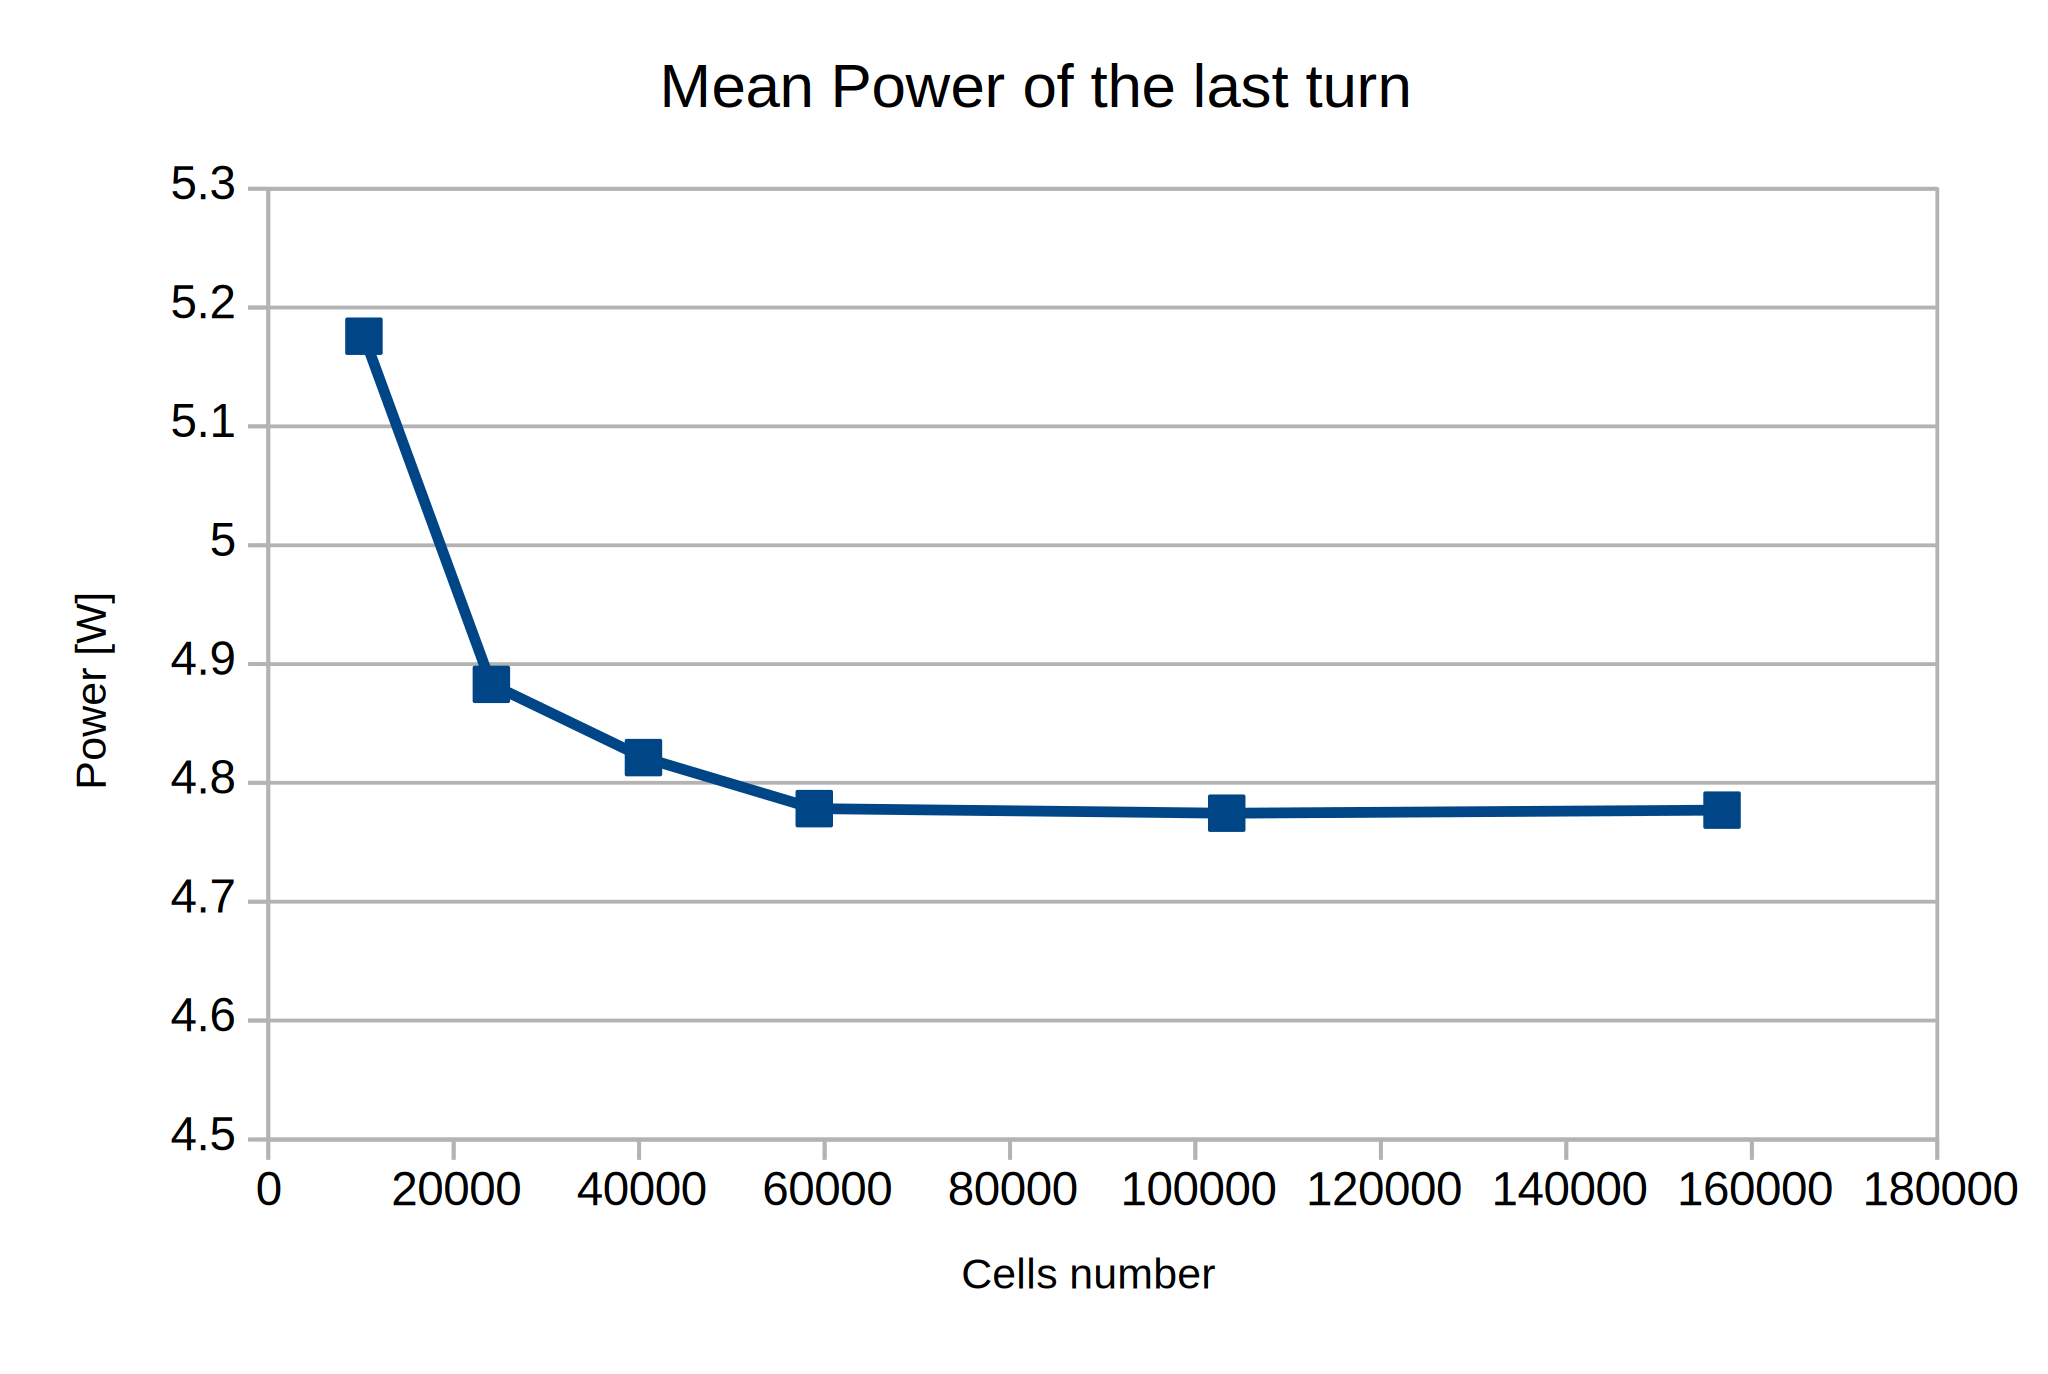
\includegraphics[width=8.5cm]{images/meshsensitivity/power-noregion}}
\subfigure[Mesh with refinement region]{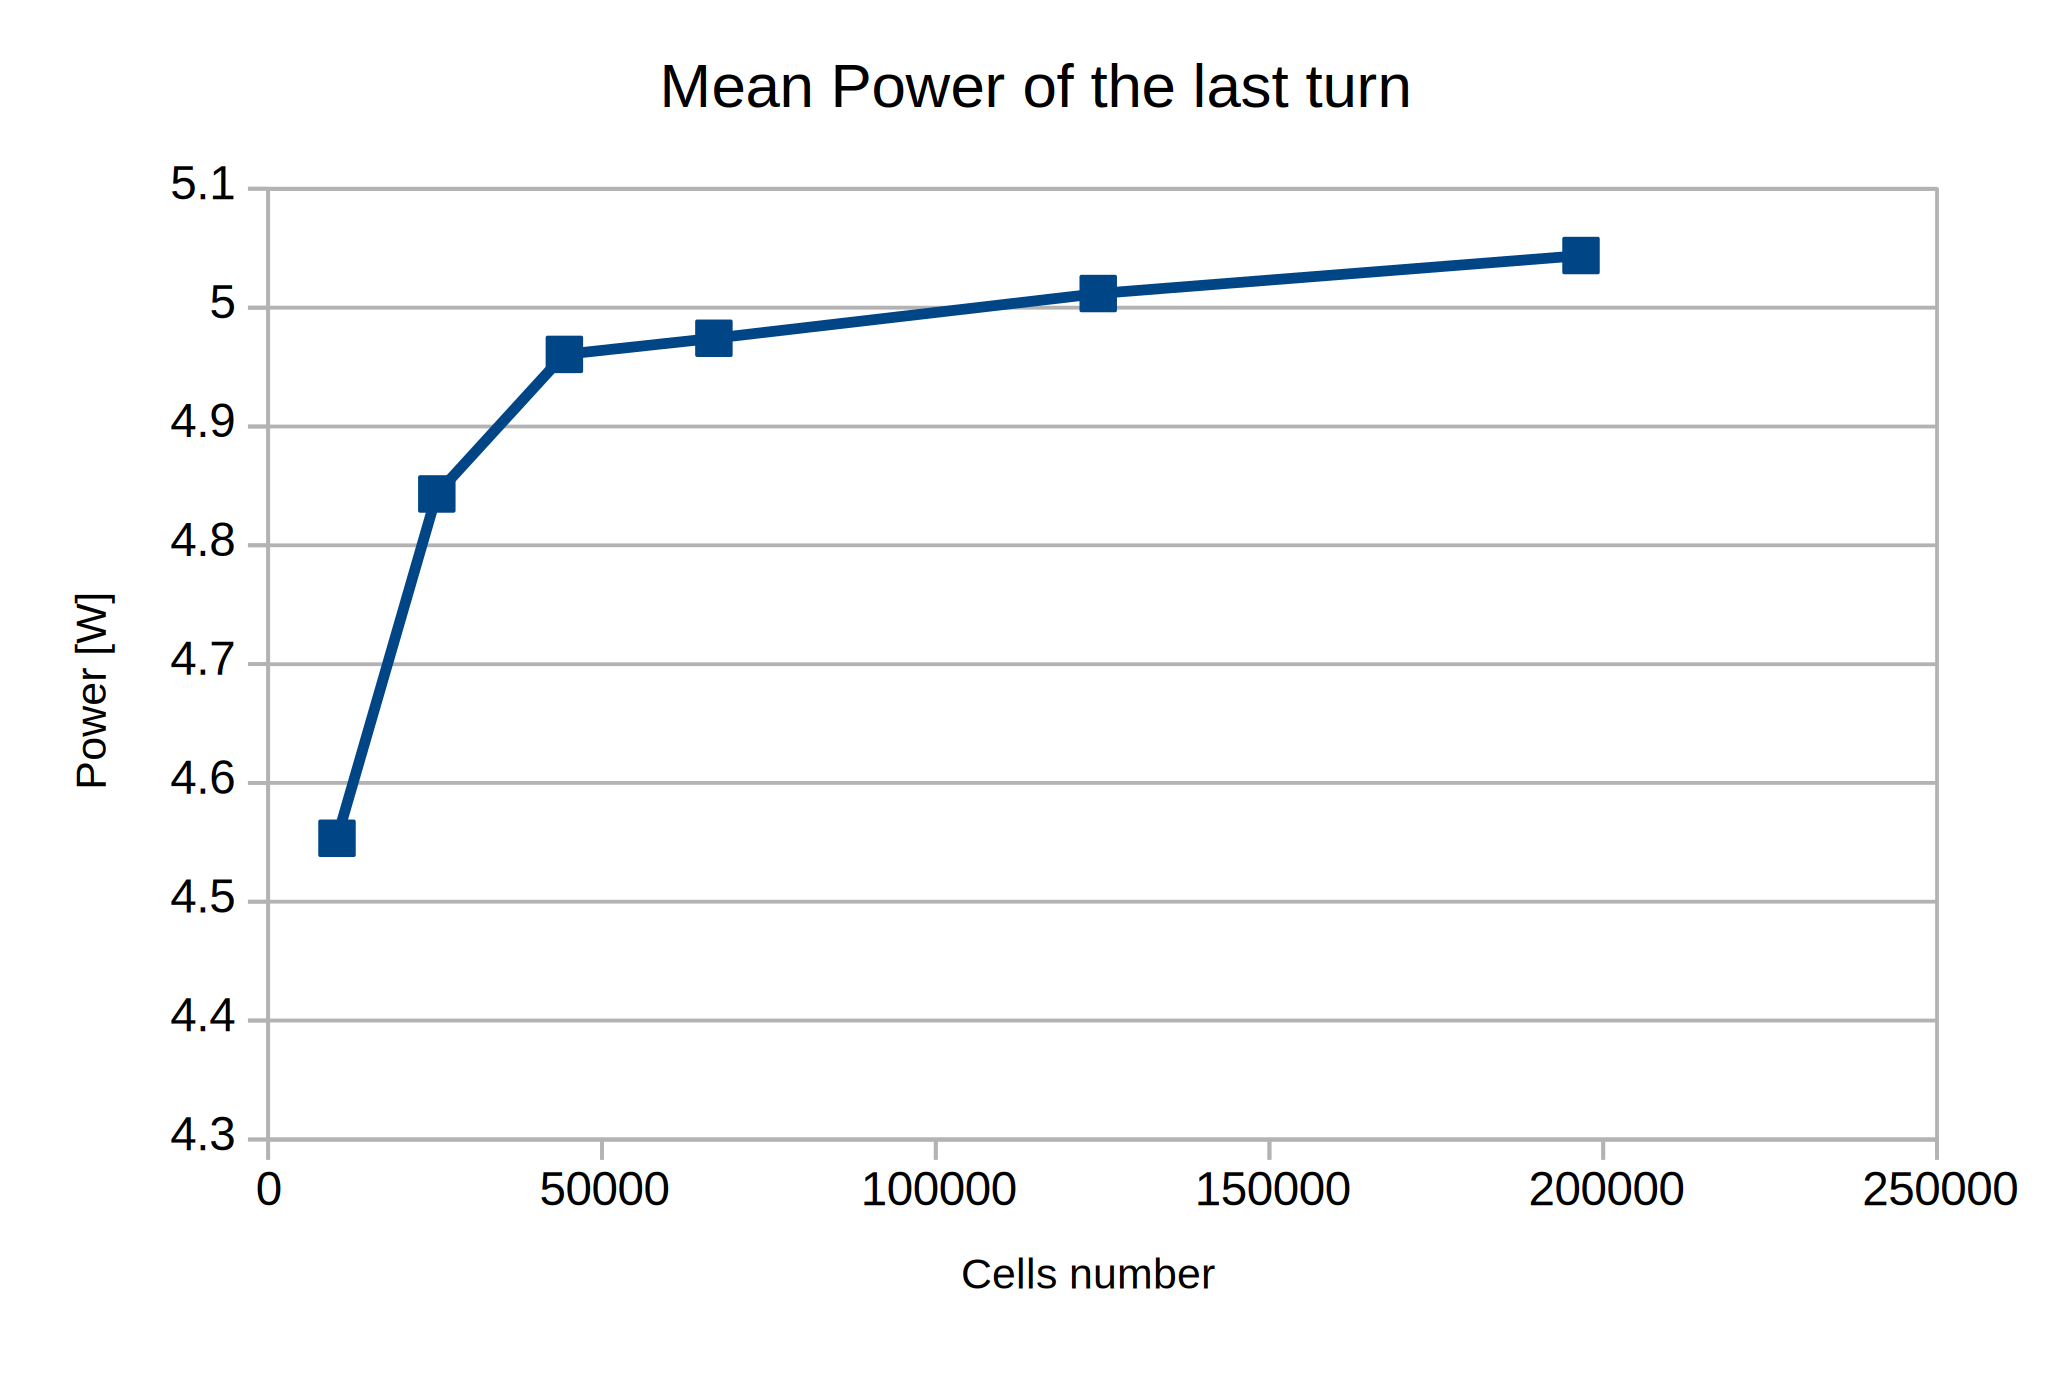
\includegraphics[width=8.5cm]{images/meshsensitivity/power-region}}
\caption{Average power in time between 1.8 and 2.4 seconds}
\label{fig:meshsensityvity-power}
\end{figure}


\begin{figure}[H]
\centering
\subfigure[Mesh without refinement region]{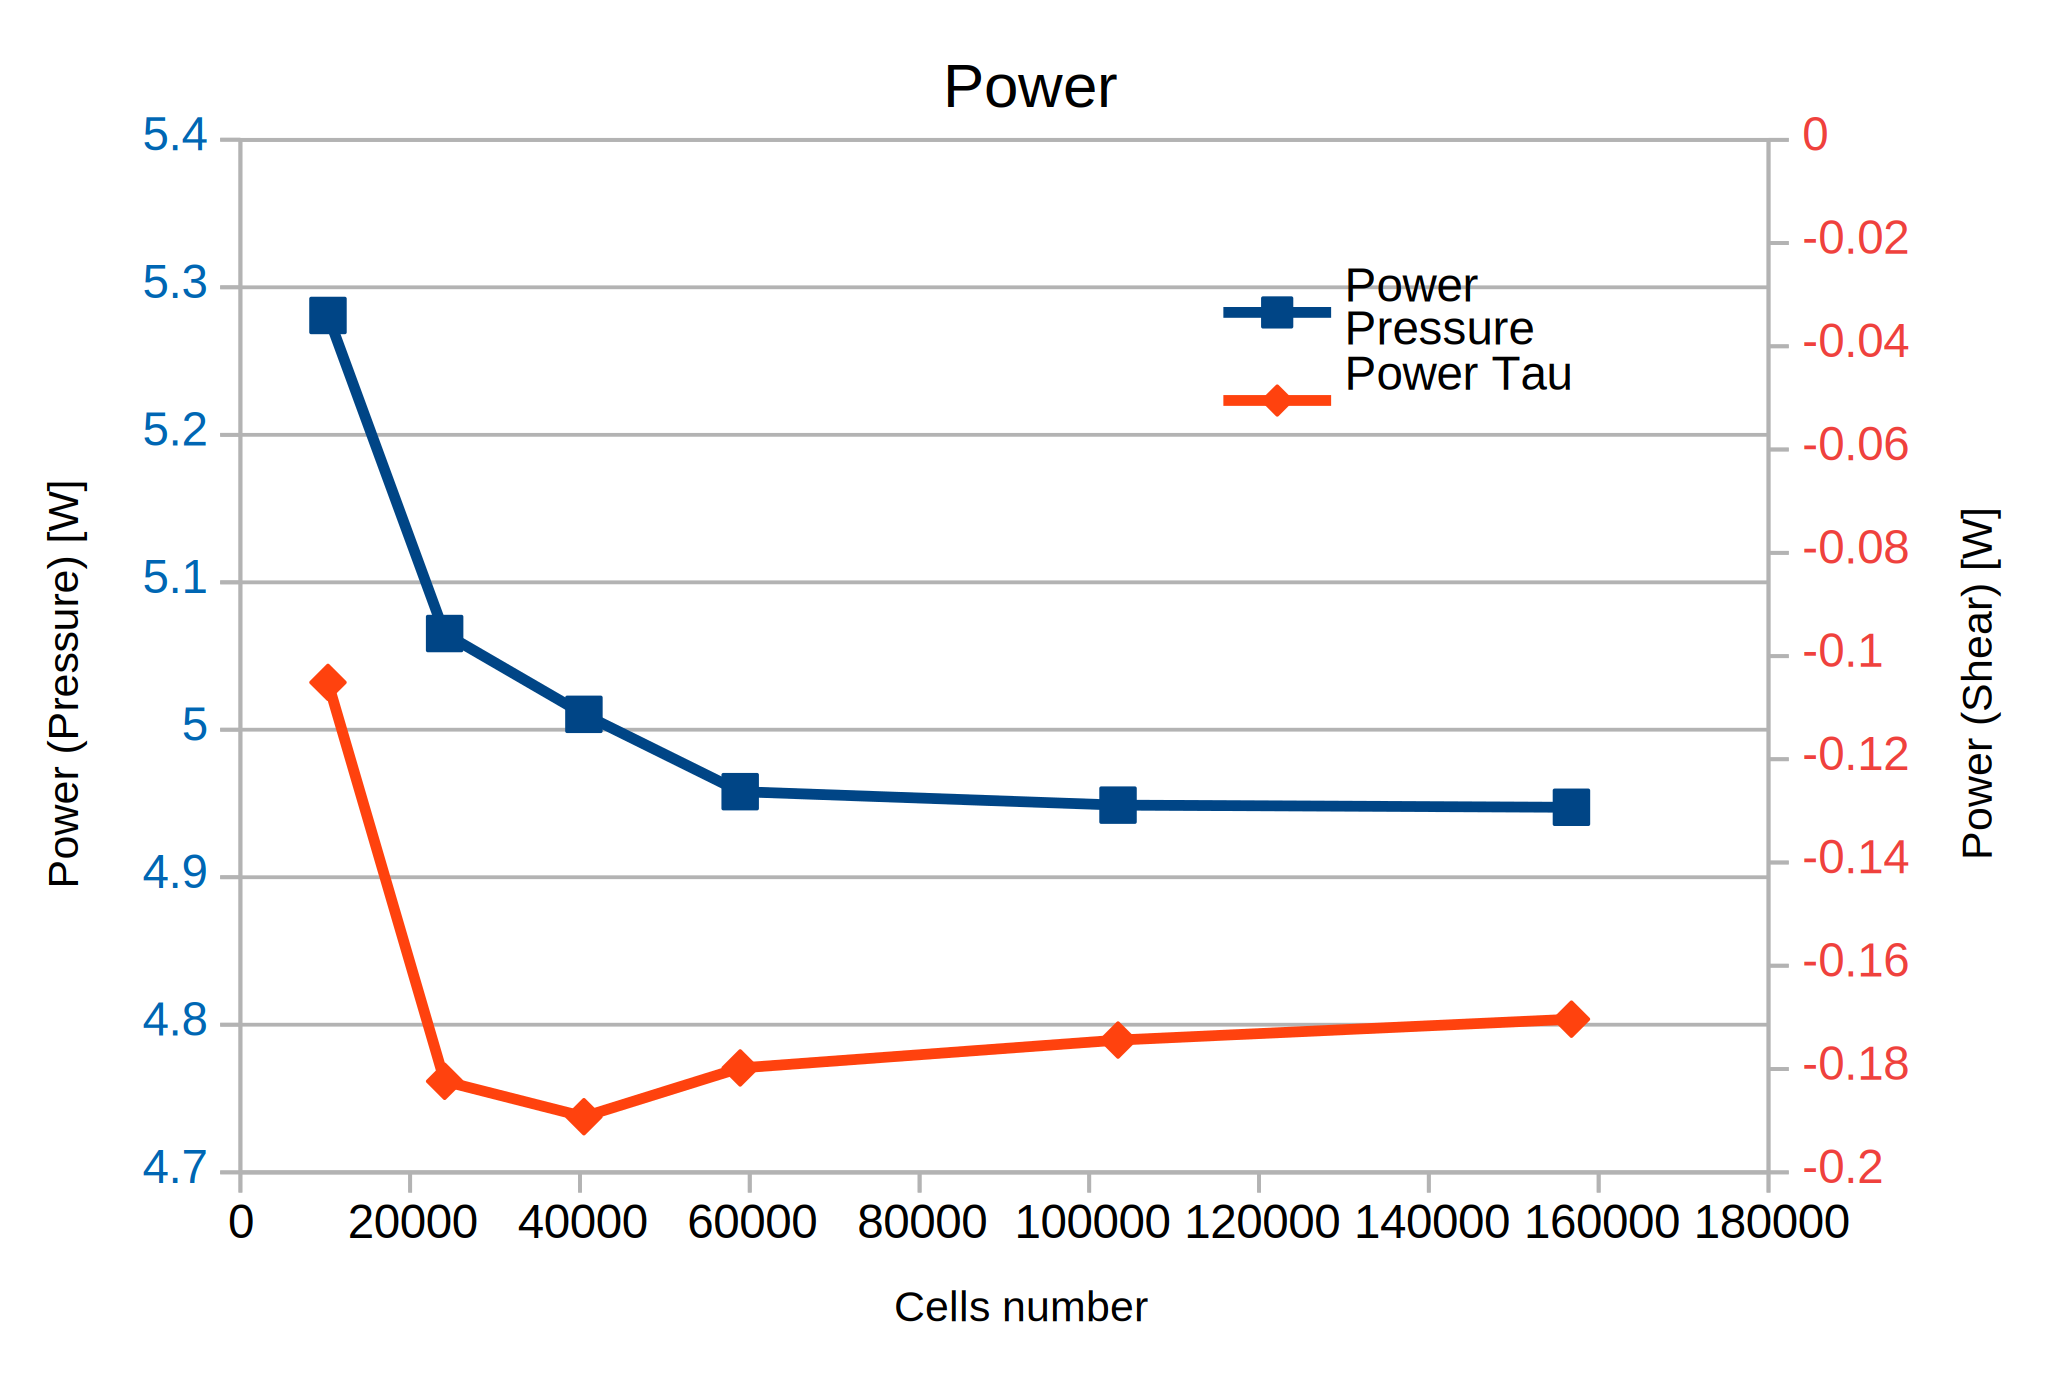
\includegraphics[width=8.5cm]{images/meshsensitivity/power-ptau-noregion}}
\subfigure[Mesh with refinement region]{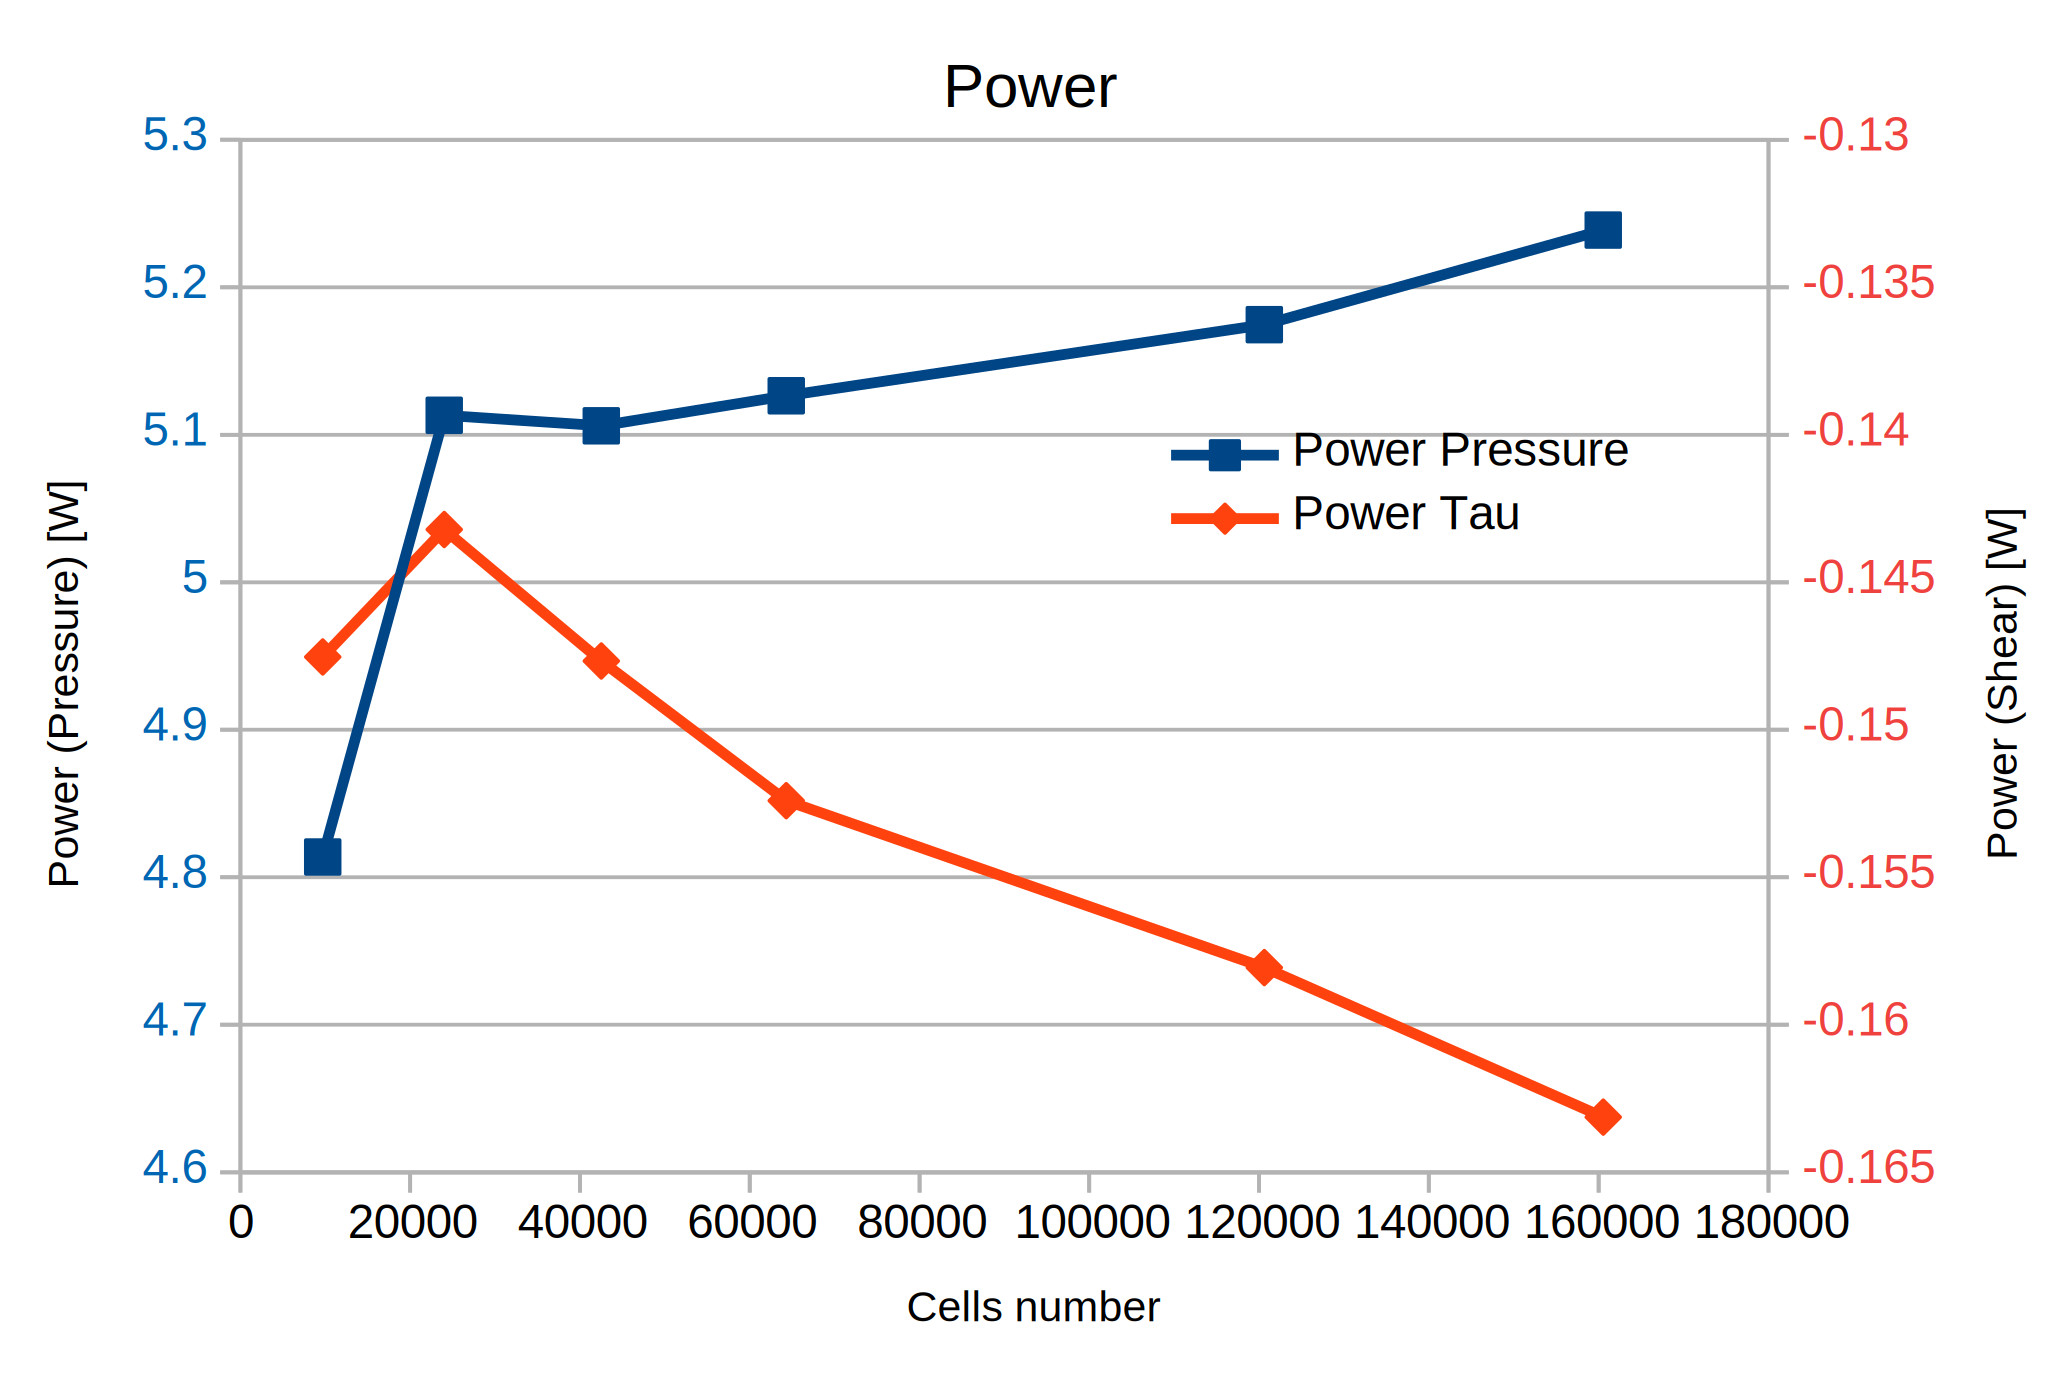
\includegraphics[width=8.5cm]{images/meshsensitivity/power-ptau-region}}
\caption{Average power in time between 1.8 and 2.4 seconds}
\label{fig:meshsensityvity-power-ptau}
\end{figure}

As we can see in figure \ref{fig:meshsensityvity-power} the power converges in both cases around mesh 80, and we get a stable convergence above mesh 120.
This fact is quite interesting since the two kind of meshes bring to slightly different results, from $4.8 \w$ to $5.0 \w$ but in both cases the mesh converges.

This result let us think that depending on the mesh we can have different results but at around mesh 120 the power result is reliable for each kind of mesh.

So in the next sections we will design a mesh which best fits the 120 cells along y direction, since the mesh used during mesh sensitivity analysis has to be applied generically between 20 and 160 cells along y axis, which is a pretty wide range.

\paragraph{Total pressure:} for the total pressure we consider 3 different cases:
\begin{itemize}
\item Total pressure average on outlet patch at 2.4 seconds.
\item Total pressure drop between inlet and outlet at 2.4 seconds.
\item Total pressure drop between reference inlet at 0 seconds and outlet at 2.4 seconds.
\end{itemize}

\begin{figure}[htbp]
\centering
\subfigure[Mesh without refinement region]{\includegraphics[width=8.5cm]{{images/meshsensitivity/totalpout-2.4-noregion}.pdf}}
\subfigure[Mesh with refinement region]{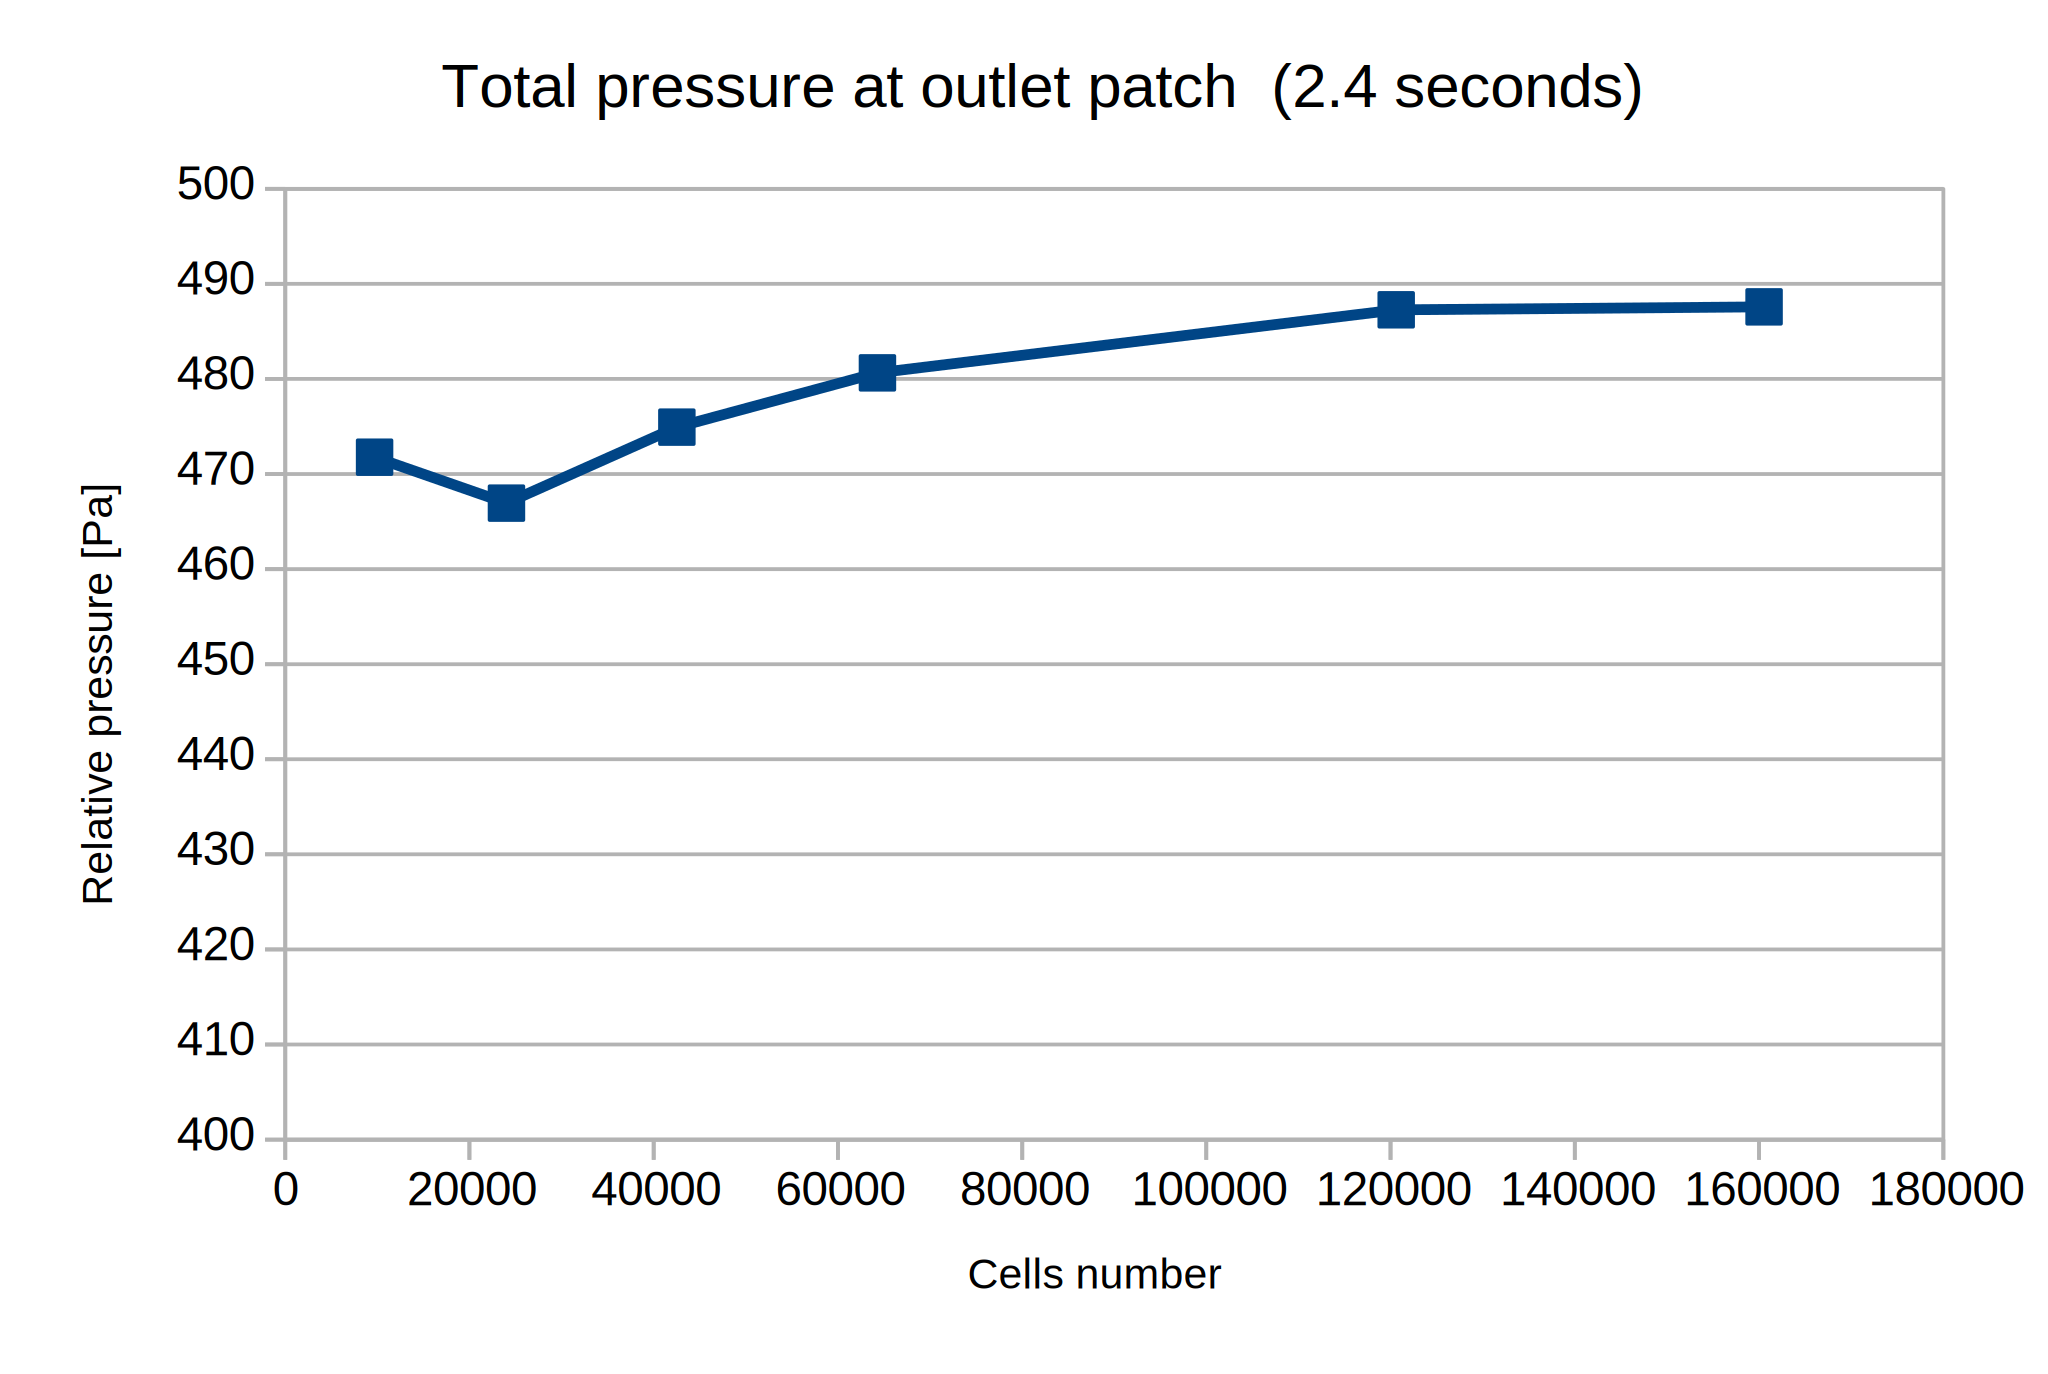
\includegraphics[width=8.5cm]{{images/meshsensitivity/totalpout-2.4-region}.pdf}}
\caption{Total pressure average on outlet patch at 2.4 seconds}
\label{fig:meshsensityvity-totalpressure-case1}
\end{figure}

\begin{figure}[htbp]
\centering
\subfigure[Mesh without refinement region]{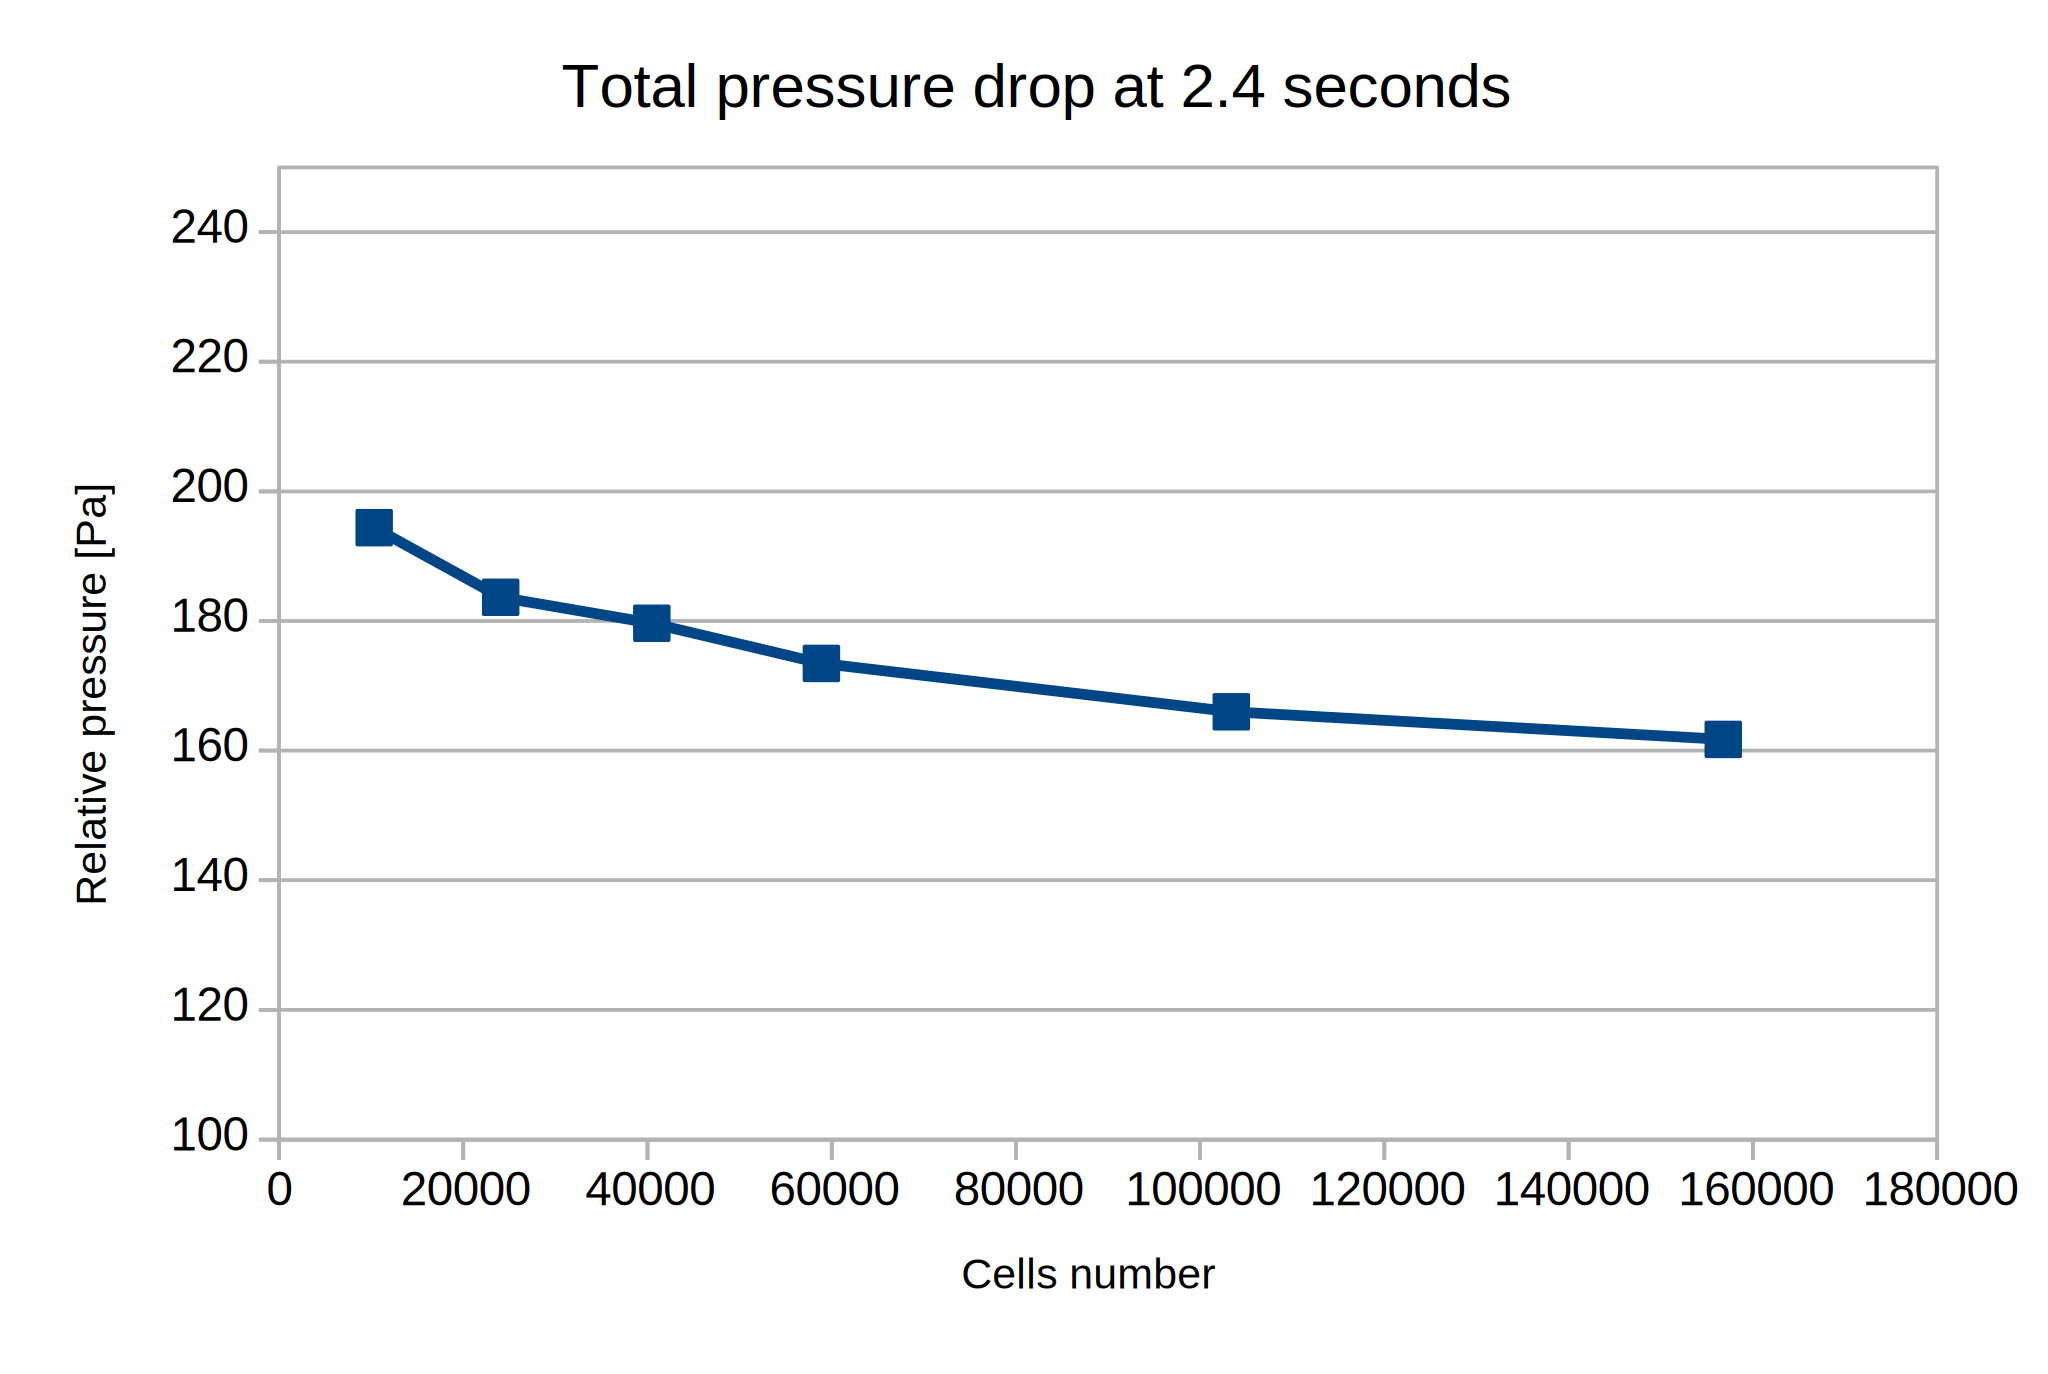
\includegraphics[width=8.5cm]{{images/meshsensitivity/totalpdrop-2.4-noregion}.pdf}}
\subfigure[Mesh with refinement region]{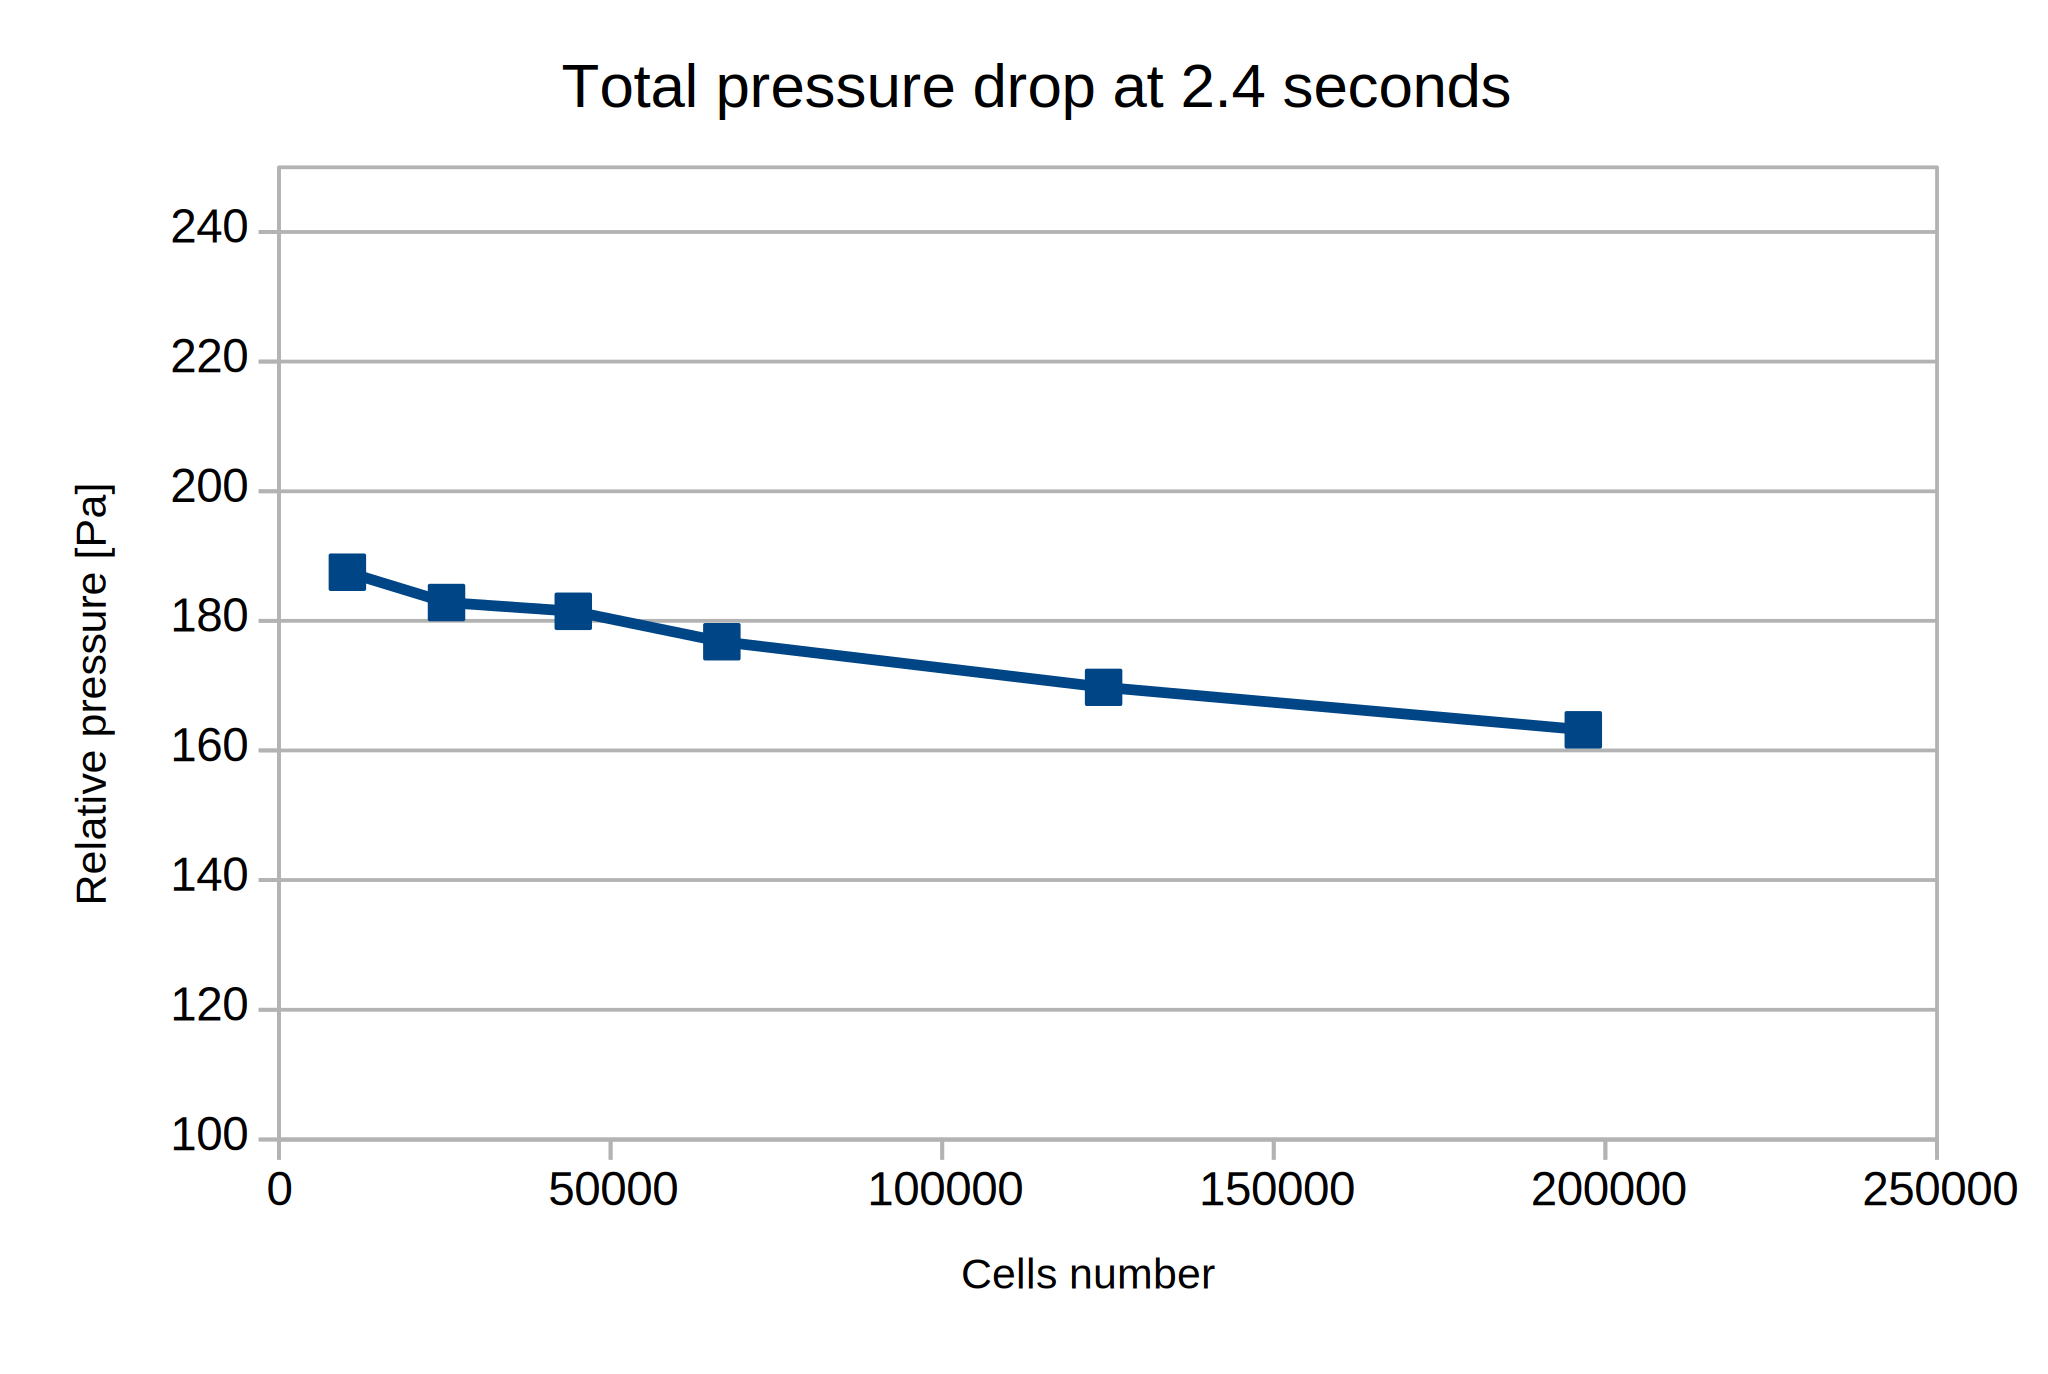
\includegraphics[width=8.5cm]{{images/meshsensitivity/totalpdrop-2.4-region}.pdf}}
\caption{Total pressure drop between inlet and outlet at 2.4 seconds.}
\label{fig:meshsensityvity-totalpressure-case2}
\end{figure}

\begin{figure}[htbp]
\centering
\subfigure[Mesh without refinement region]{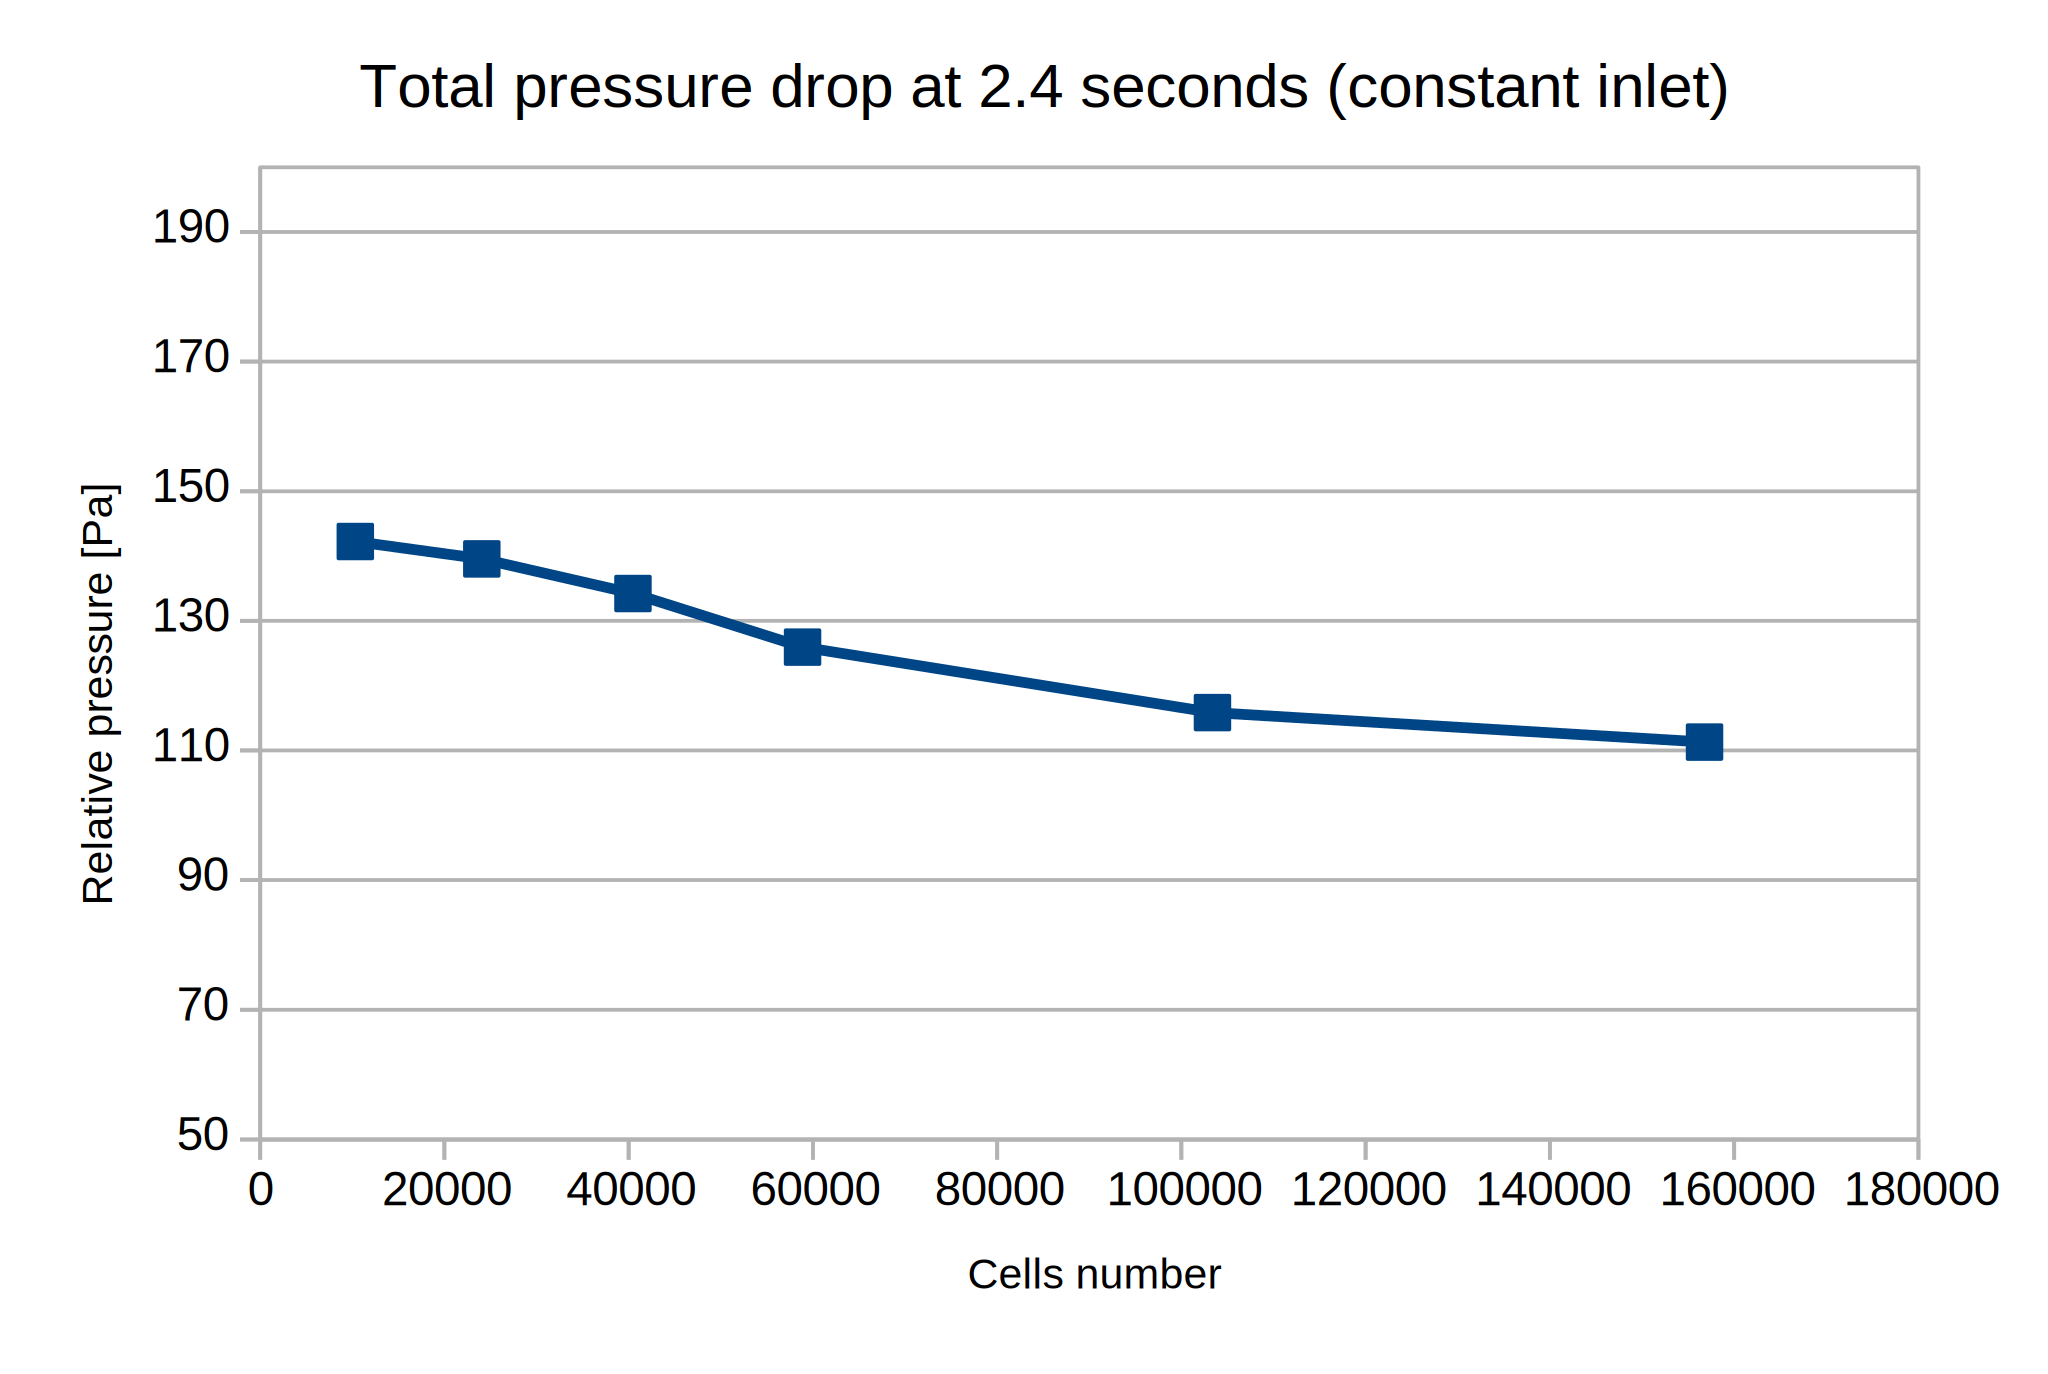
\includegraphics[width=8.5cm]{{images/meshsensitivity/totalpdrop-constantref-noregion}.pdf}}
\subfigure[Mesh with refinement region]{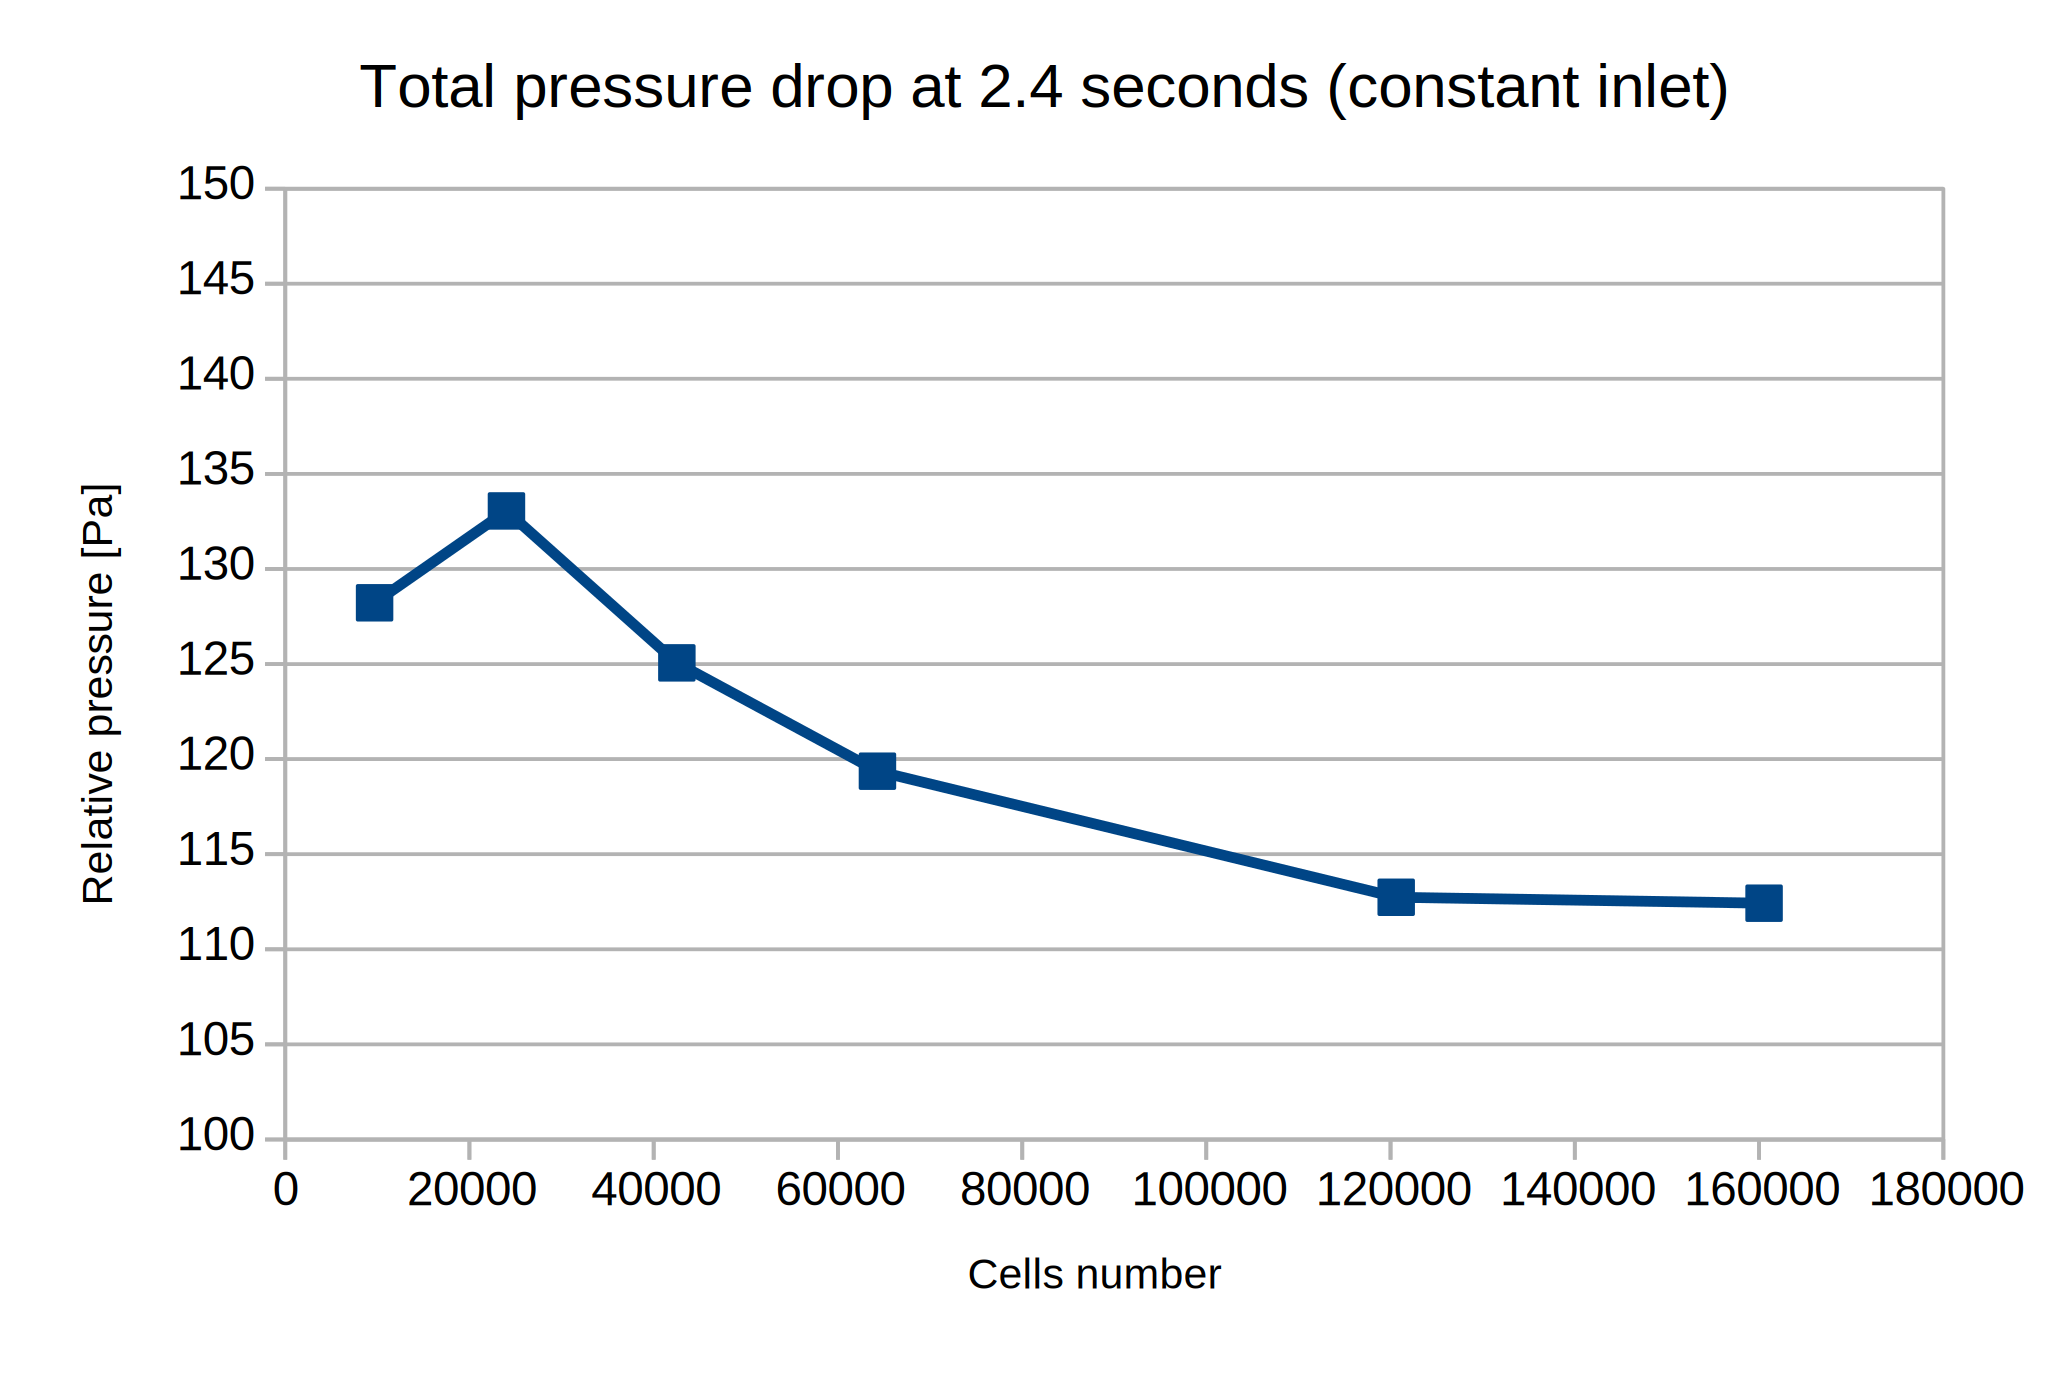
\includegraphics[width=8.5cm]{{images/meshsensitivity/totalpdrop-constantref-region}.pdf}}
\caption{Total pressure drop between reference inlet at 0 seconds and outlet at 2.4 seconds.}
\label{fig:meshsensityvity-totalpressure-case3}
\end{figure}

Some cases show a great convergence at mesh 120, some others highlight the fact that probably the best possibility is to go towards mesh 160, even though the difference is in general small.

Due to limitation in computational time we stay in the middle between mesh 80 which seems good from the point of view of the power and mesh 160 which seems the best even in any case.

To let us perform more analysis in next chapter and balancing the fact that power shows a good convergence we will choose mesh 120 to perform further simulation if not explicitely specified.

\section{Final mesh}

As we have said before we will design a proper mesh that fits with 120 cells in y direction.
Up to now we have applied one layer with snappyHexMesh around the blades and then we have splitted it with refineWallLayer four times.
Now the aim is to create the biggest layer as possible with snappyHexMesh, divide that region with a proper number of layer with snappy, and then divide once more the last layer with refineWallLayer utility.
\\
We manage to obtain 4 layer with snappyHexMesh and then we apply refineWallLayer 3 further times.

Then we add a refinement region of 3 levels around each blade with an extension of $4 \mm$

We keep 2 layers per region where we have contact between moving surfaces. The total number of layer around Ami patches so will be equal to 4, two per side.

\begin{figure}[hbtp]
\centering
\includegraphics[width=17cm]{images/mesh-120/view-full.png}
\caption{Full view of the mesh}
\end{figure}

\begin{figure}[htbp]
\centering
\subfigure[Blade tip region.]{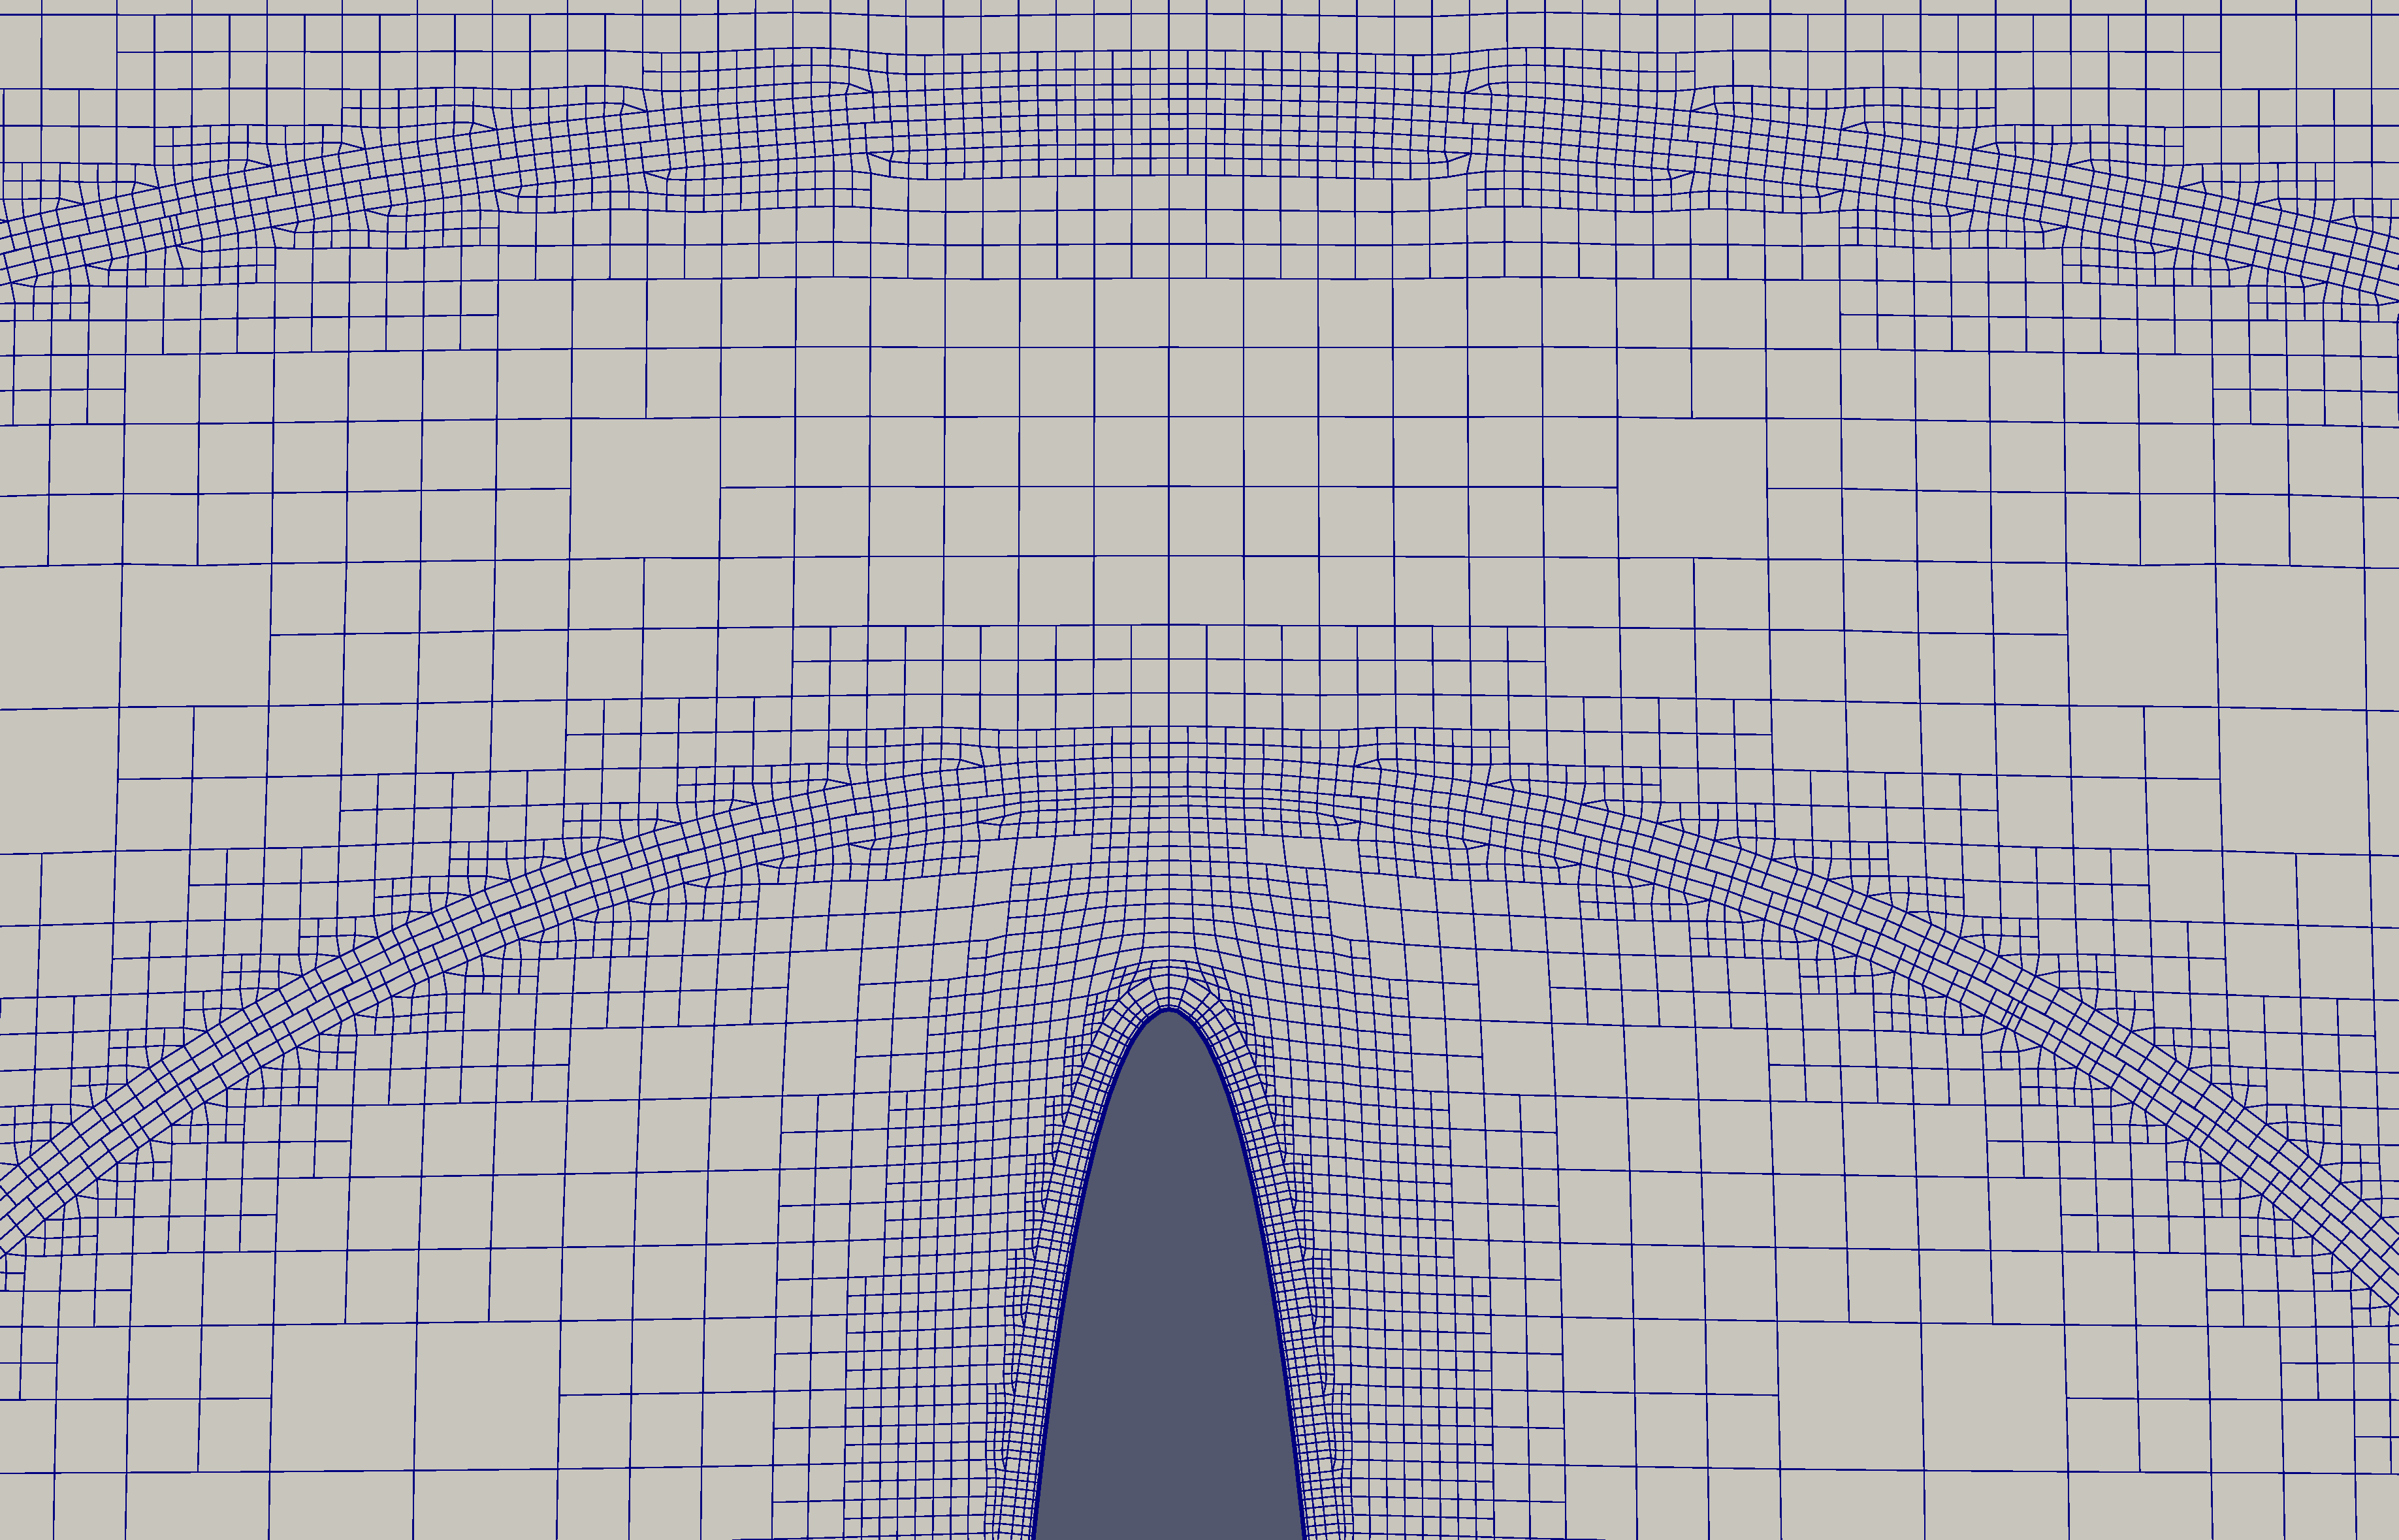
\includegraphics[width=8.5cm]{{images/mesh-120/view-bladetip}.pdf}}
\subfigure[Boundary layer.]{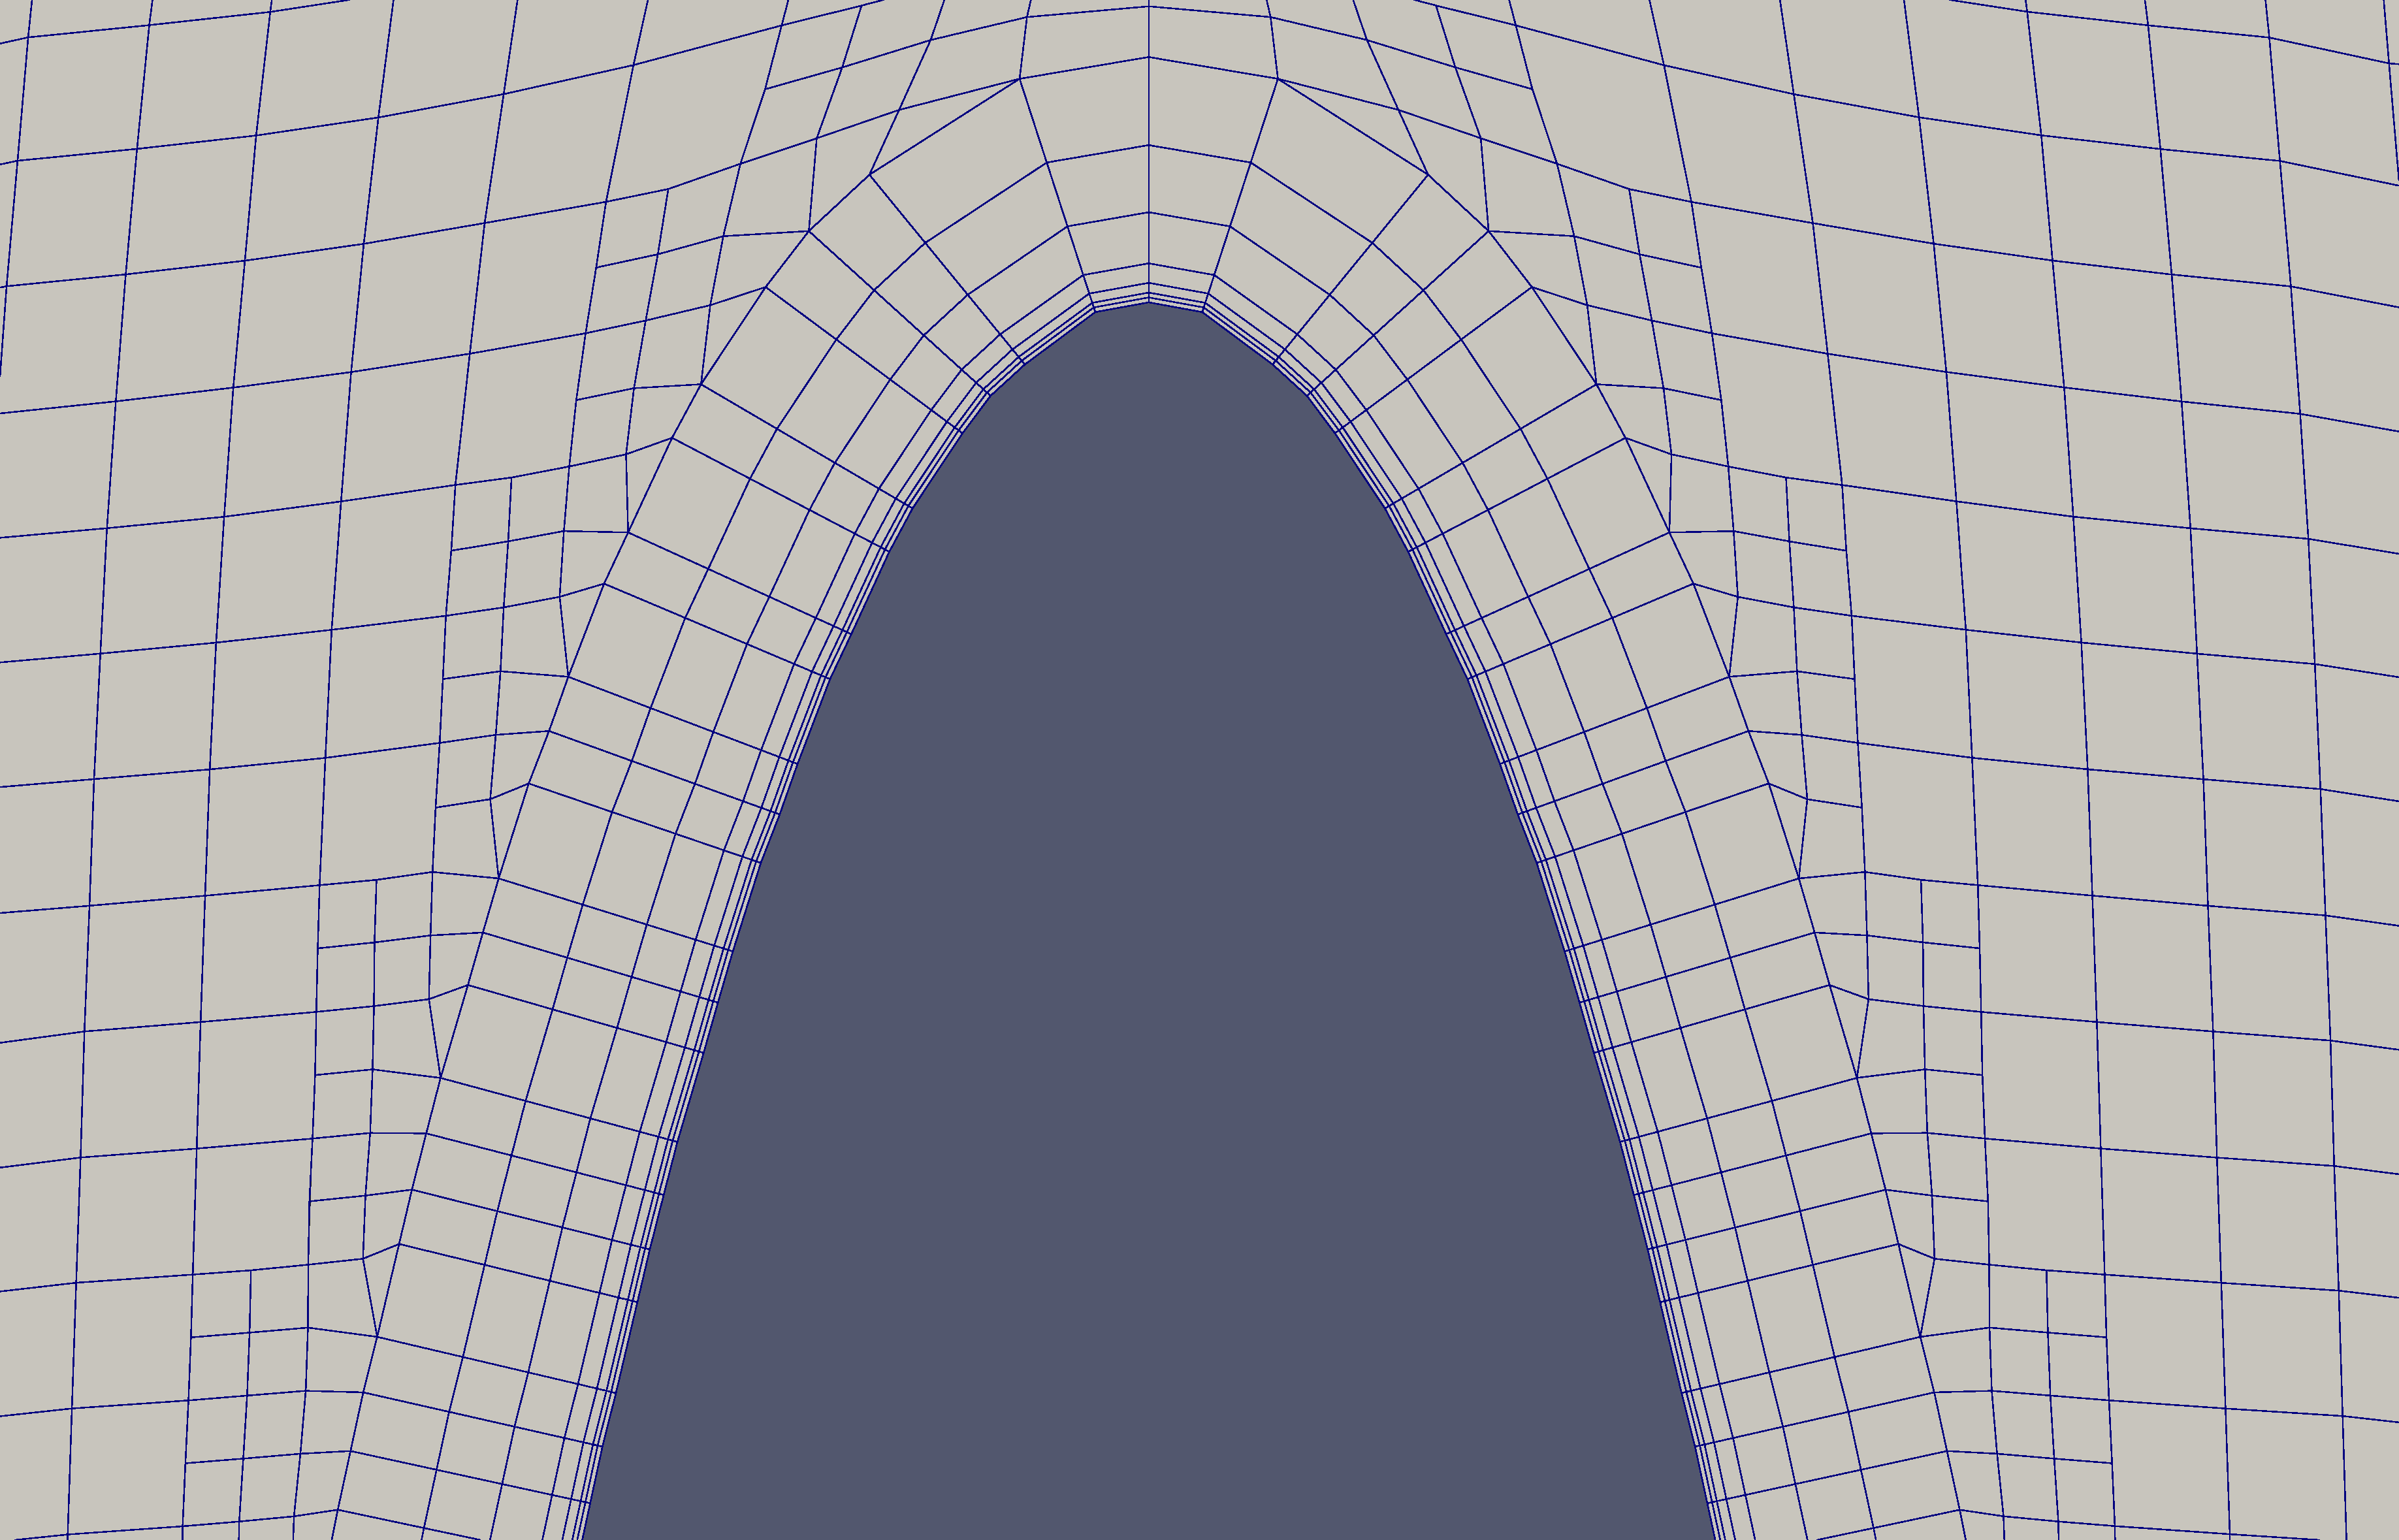
\includegraphics[width=8.5cm]{{images/mesh-120/view-bladetip-zoom}.pdf}}
\end{figure}

\begin{figure}[H]
\centering
\includegraphics[width=17cm]{images/mesh-120/view-blade0.pdf}
\caption{View of the blade 0 at time 0 seconds}
\end{figure}

We finally obtain a mesh whose characteristics are displayed in table \ref{table:mesh120}. All the properties, both that represented and all the others, respect our limits of the mesh quality control. 
\begin{table}[H]
\centering
\caption{Properties of the mesh}
\label{table:mesh120}
\begin{tabular}{lr|c}
\toprule
Cells                 & $113754$     &    \\
Max Skewness          & $2.71645$    & OK \\
Max non-orthogonality & $58.52\,^{\circ}$ & OK \\
Max aspect ratio      & $16.1092$    & OK \\ \bottomrule
\end{tabular}
\end{table} 

\section{Numerical Schemes}
The file which menage the numeric scheme is in \textit{fvSchemes}. Inside that file it is possible to define the scheme used for the calculation of many terms, specified in the following section. All of them are necessary to be able to discretize all the terms inside the continuity and momentum equation:
\begin{itemize} 
 \item time derivative terms inside \textit{timeSchemes};
 \item gradient terms $\nabla$ inside \textit{gradScheme};
 \item divergence terms $\nabla\cdot $ inside \textit{divSchemes};
 \item laplacian terms $\nabla^2$ inside \textit{lapSchemes};
 \item cell to face interpolation schemes  inside \textit{interpolationSchemes};
 \item component of gradient normal to a cell face  inside \textit{snGradSchemes}.
 \end{itemize} 
It is possible to define specific scheme for each term of the equation, however our decision was to use as much as we can the default scheme. 
In addition from a very large amount of scheme only those used in the tutorial cases of openFoam were tested. This research can be simply done by using the command \foam{foamSearch}.

%%%%%%%%%%%%%%%%%%%%%%%%%%%%%%%%%%%%%%%%%%%%%%%%%%%%%%%%%%%%
In the next sub paragraphs we present an overviwe of different schemes and their characteristics \footnote{https://www.openfoam.com/documentation/user-guide/fvSchemes.php} \footnote{https://cfd.direct/openfoam/user-guide/fvschemes/} \footnote{https://www.openfoam.com/documentation/cpp-guide/html/guide-schemes.html}
%%%%%%%%%%%%%%%%%%%%%%%%%%%%%%%%%%%%%%%%%%%%%%%%%%%%%%%%%%%%

Since the scheme are a lot and the combination between them will be huge, our decision was to focus only on the influence of one scheme, keeping fixed all the others. The reference case to study the differences is the base case, used in class, which is the same used for the tutorial case:
 %% inserisci tabella 1
\begin{table}[H]
\begin{tabular}{ll}
\toprule
Section          & \foam{Scheme used }                               \\ \midrule
ddtSchemes       & \foam{default         Euler}                      \\
gradSchemes      & \foam{default         Gauss linear}               \\
divSchemes       & \foam{default         none}                       \\
                 & \foam{div(phi,U)      Gauss upwind}               \\
                 & \foam{div(phi,k)      Gauss upwind}              \\
                 & \foam{div(phi,epsilon) Gauss upwind}              \\
                 & \foam{div(phi,omega) bounded Gauss upwind}        \\
                 & \foam{div((nuEff*dev2(T(grad(U))))) Gauss linear} \\
                 & \foam{div(nonlinearStress) Gauss linear}          \\
laplacianSchemes & \foam{default         Gauss linear corrected}     \\
snGradSchemes    & \foam{default         corrected   }              \\ \bottomrule
\end{tabular}
\end{table}

The comparison has been done looking at:
\begin{itemize} 
 \item power generated by the turbine;
 \item power generated by pressure only;
 \item power dissipated by the effect of the shear stress;
 \end{itemize} 

\subsection{Interpolation schemes}
Specify the scheme for moving proprieties for cell center to face center. These operation is included in the calculation of gradient, divergence and laplacian terms. An overview of interpolation schemes are:

\begin{table}[H]
\centering
\begin{tabular}{ll}
\toprule
Scheme          & Numerical behaviour                           \\ \midrule
linear          & linear interpolation (central differencing)   \\
cubicCorrection & Cubic scheme                                  \\
midPoint        & Linear interpolation with symmetric weighting \\ \bottomrule
\end{tabular}
\caption{General interpolation schemes}
\label{table:interpolation_general}
\end{table}

\begin{table}[H]
\centering
\begin{tabular}{ll}
\toprule
Scheme                                    & Numerical behaviour                              \\ \midrule
upwind (upwind convection group)          & Upwind differencing                              \\
linearUpwind (upwind convection group)    & Linear upwind differencing                       \\
skewLinear (upwind convection group)      & Linear with skewness correction                  \\
filteredLinear2 (upwind convection group) & Linear with filtering for high-frequency ringing \\
limitedLinear (TVD schemes)               & limited linear differencing                      \\
vanLeer (TVD schemes)                     & van Leer limiter                                 \\
MUSCL (TVD schemes)                       & MUSCL limiter                                    \\
limitedCubic (TVD schemes)                & Cubic limiter                                    \\
SFCD (NVD schemes)                        & Self-filtered central differencing               \\
Gamma $\psi$  (NVD schemes)               & Gamma differencing                               \\ \bottomrule
\end{tabular}
\caption{Gaussian discretization of convection}
\label{table:interpolation_convection}
\end{table}

% up to now %%%%%%%%%%%%%%%%%%%%%%%%%%%%%%%%%%%%%%%%%%%%%%%%%%%%%

For our calculation, only linear scheme has been adopted. Second group of schemes interpolate on the basis of the flux of the flow velocity. For this reason they require the name of the flux field used for interpolation.


\subsection{Normal gradient schemes}
The gradient is calculated from cell center, and then interpolated. 
\\The normal contribution will be: 
\begin{equation}
\nabla_f Q = \hat{n} \cdot (\nabla Q )_f
\end{equation}

where $\hat{n}$ is the face unit normal. It controls the scheme for the calculation on the gradient normal to cell face, in the middle of the face in between two cells. available schemes are : \\
\begin{itemize} 

 \item {\ttfamily corrected} : Central-difference snGrad scheme with non-orthogonal correction, explicit.
  \item {\ttfamily uncorrected}: no correction of the orthogonality.
 \item {\ttfamily limited $\psi$}: which requires another input, in between 1 and 0, where 1 correspond to correct scheme while 0 correspond to uncorrect scheme. So it is a weighted bland between the two.
 \item {\ttfamily bounded}: bounded correction for positive scalars
 \item {\ttfamily fourth} : fourth order scheme.
\end{itemize} 

The use of different scheme will be discussed in laplacian section.

\subsection{Time schemes}
Time schemes define the way in which a propriety is integrated in time. Depending on the choice of the user, an old $\phi^0$ or old-old $\phi^{00}$ solution will be required.
The different schemes analyzed are:
\begin{itemize} 
 \item {\ttfamily steadyState}: used for steady state simulation where there's no time derivative, so to analyze a steady problem.
 
 \item {\ttfamily localEuler}: first order,implicit, psuedotransient used for accelerating the convergency to a steady state problem,.
 
 \item {\ttfamily Euler}: implicit, first order, transient used for unsteady problem.
\begin{equation}
\frac{d \phi}{dt} = \frac{\phi - \phi^0}{\Delta t}
\end{equation} 

 
 \item {\ttfamily backward}: implicit, second order, transient, conditionally stable and boundness is not guaranteed.
\begin{equation}
\frac{d \phi}{dt} = \frac{1}{\Delta t}\left(\frac{3}{2}\phi - 2\phi^0- \frac{1}{2}\phi^{00}\right)
\end{equation} 
 
 \item {\ttfamily CrankNicolson}: second order, transient, bounded. \\for uniform time step the scheme is equal to:
\begin{equation}
 \frac{d \phi}{dt} = \frac{\phi - \phi^{00}}{2\Delta t}
\end{equation} 
 
To assure stability it is possible to adopt a blend with Euler system, with a coefficient in between 0 and 1, where 0 rappresent pure Euler while 1 rapprensent pure CrankNicolson.
 
 \end{itemize} 
 For second derivative scheme (not present in our equation) only Euler scheme is possible.

\paragraph{Results} \mbox{}\\
The different type of schemes are reported in the following figure, with the relative scheme used. The comparison is made considering the overall power produced by the turbine, the ideal power, related to the effect of the pressure only and the power loss associated to the shear stress action:
\begin{figure}[H]
\centering
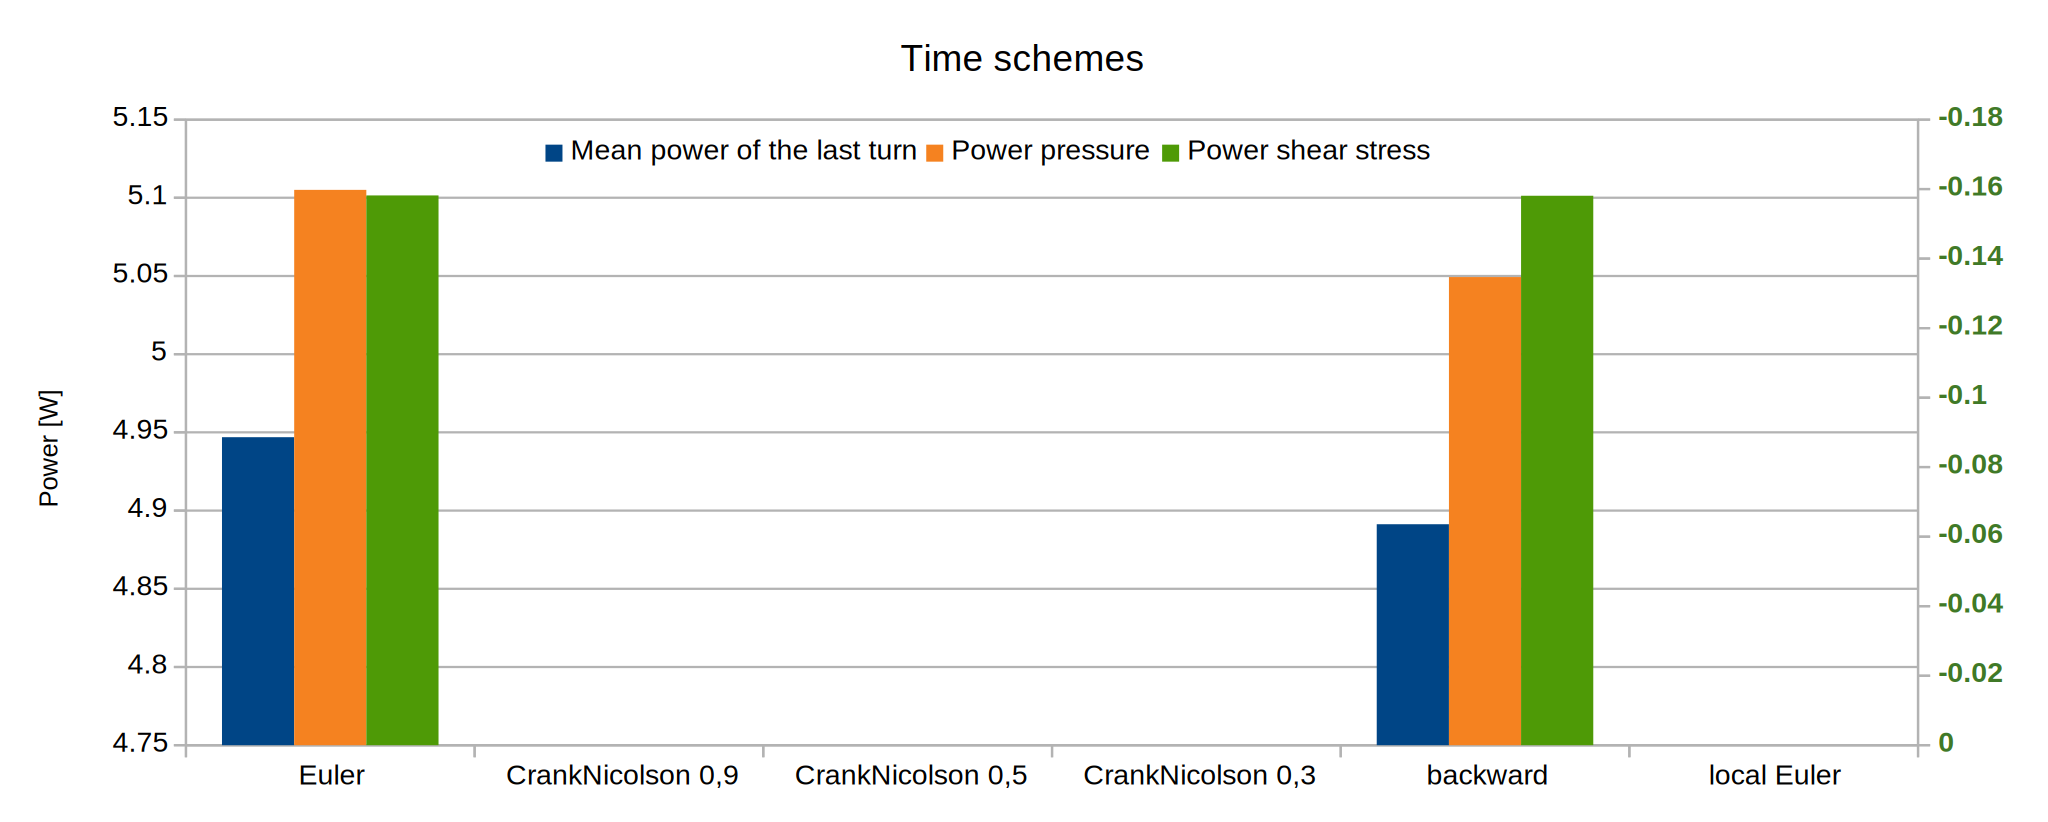
\includegraphics[height=6cm]{images/schemes/timeschems-results.pdf}
\end{figure}

CrankNicolson scheme with different blending coefficient has been tested, however it will cause instability which lead the residual to rise after 0.003s for CrankNicolson0.3 after 0.005s for CrankNicolson0.5 and 0.0045s for CrankNicolson0.9.
Even if backward scheme is a purly second order scheme (so in theory more prone to instability), it works.
No difference can be seen in the shear stress power loss, but for ideal power (related to pressure) backward scheme will provide a different value, 1\% less. The time required for the calculation is 6\% higher and the values of the residual are of the same order of magnitude.



\subsection{Gradient schemes}
The gradient of a certain quantity $\phi$ rappresent the way in which that propriety is changing along a direction. For a scalar quantity $\phi$
 
\begin{equation}
\nabla \phi = \begin{bmatrix} \frac{\partial \phi}{\partial x} \\ \frac{\partial \phi}{\partial y} \\\frac{\partial \phi}{\partial z}\end{bmatrix} 
\end{equation}

The different schemes analyzed are:
\begin{itemize} 
 \item {\ttfamily Gauss linear}: Gauss specify that the scheme used, in these case the Gaussian integration, which requires the interpolation from cell center to face centres. Therefore second input specify the scheme used for interpolation, in these case linear interpolation or central differencing.
 
 \item {\ttfamily leastSquares}: second order scheme which uses all neighbouring cells to calculate distance with least square scheme.
 
 \item {\ttfamily Gauss cubic}: third-order schemes, typically used in very regular mesh.
 \end{itemize} 
 
 
\paragraph{Results} \mbox{}\\
The different type of schemes are reported in the following figure, with the relative scheme used. 
\begin{figure}[H]
\centering
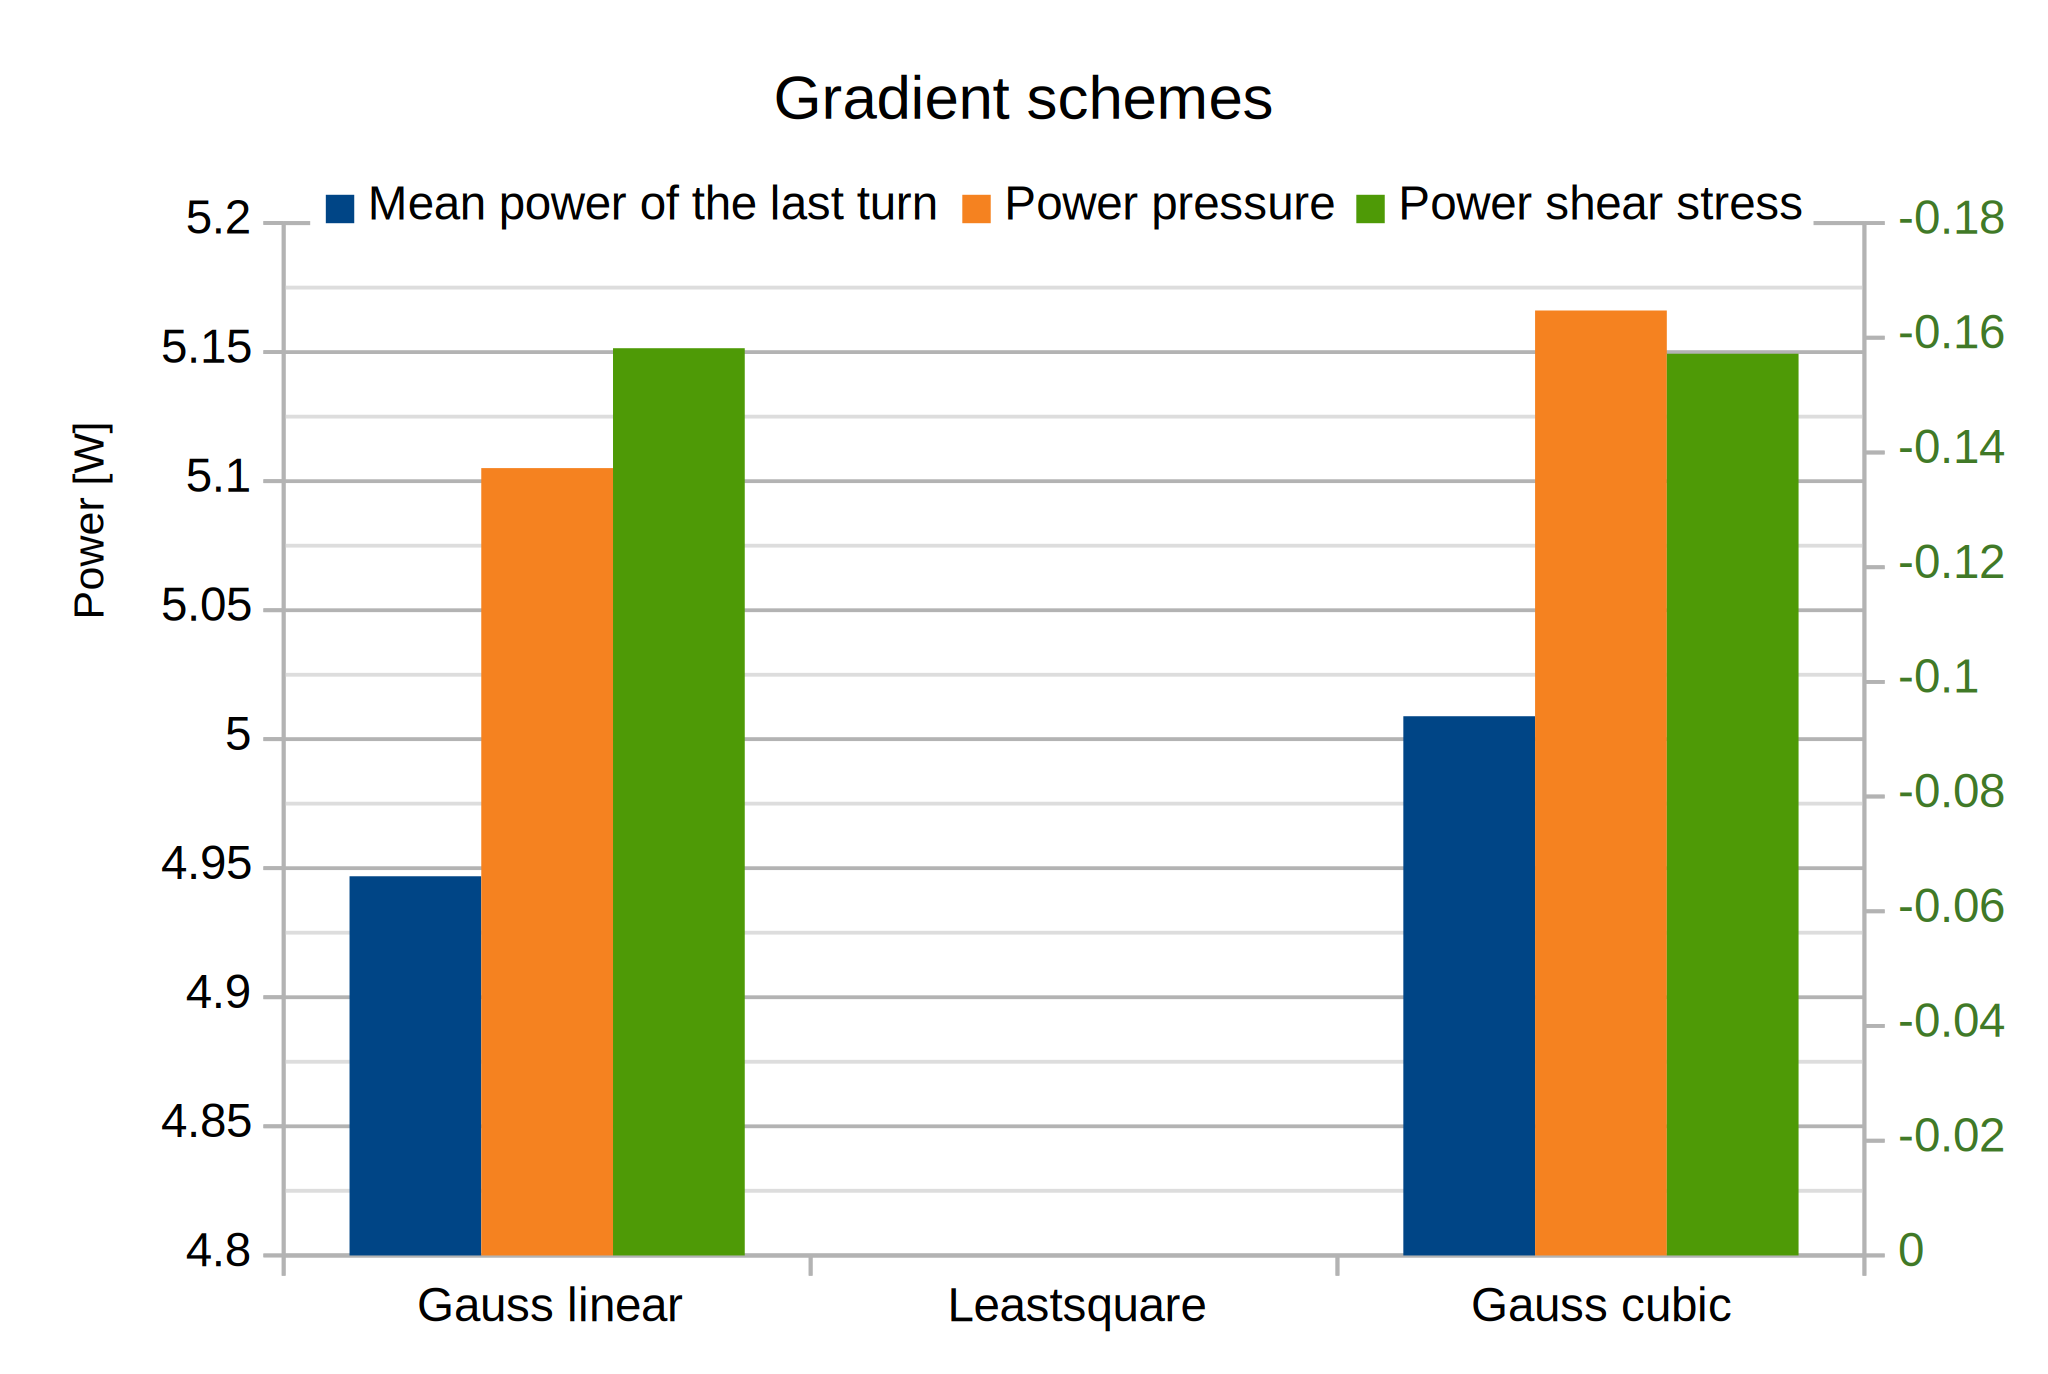
\includegraphics[height=6cm]{images/schemes/gradschems-results.pdf}
\end{figure}
Leastsquare scheme doesn't work, and simulation does not start. The gauss cubic scheme, instead works properly.
As for time schemes, no difference can be seen in the shear stress power loss (arounf 0.6\%), while for pressure power, cubic schemed differs to linear for 1\%. The time required for the calculation is 18\% higher and the values of the residual are comparable.

\subsection{Divergence schemes}
The divergence of a propriety $\bm{U}$ rappresent the rate at which that quantity is changing.
\begin{equation}
 \nabla \cdot \bm{U} = \frac{\partial U_x}{\partial x}+ \frac{\partial U_y}{\partial y} + \frac{\partial U_z}{\partial z} 
\end{equation}


Only in this case since divergent terms are very dissimilar, it is preferable not to use a default scheme, equal to all the terms but to specify a specific sceme for each term. In addition, considering that the scheme availble are a lot, and we have:
\begin{itemize} 
 \item divergence of velocity;
 \item divergence of turbulent kinetic energy;
 \item divergence of $\omega$ and/or $\epsilon$ depending on the turbulence model chosen;
 \item divergence of shear stress;
  \item divergence of the effective viscous stress; %due to turbulence
\end{itemize} 
So our choice is to concentrate ourself on the trial of different schemes for the divergence of the velocity field.
 $ \nabla \cdot ( \rho \, \bm{U} \bm{U} )$
\\ An overview of all the scheme availble is reported below:


\begin{table}[H]
\centering
\begin{tabular}{ll}
\toprule
Scheme         & Numerical behaviour                                                               \\ \midrule
linear         & second order, unbounded (good for LES calculations due to low dissipation) \\
skewLinear     & Second order, (more) unbounded, skewness correction                               \\
cubicCorrected & Fourth order, unbounded                                                           \\
upwind         & First order, bounded                                                              \\
linearUpwind   & First/second order, bounded                                                       \\
QUICK          & First/second order, bounded                                                       \\
TVD schemes    & First/second order, bounded                                                       \\
SFCD           & Second order, bounded                                                             \\ \bottomrule
\end{tabular}
\caption{Divergence schemes}
\label{table:divergence}
\end{table}

NVD and TVD provide a blend between low order schemes and higher order schemes based on the calculation of a limiter. Boundness is ensured only for 1D problem, while 2D and 3D boundness can be imporeved limiting the gradient.

From tutorial case we found many schemes, but only those reported below are working:
\begin{itemize} 
\item {\ttfamily Gauss upwind}: first order, bounded. The face value is set according to upstream value. It forces the cell value to be constant and equal to the mean value.
 
 \item {\ttfamily Gauss linearUpwind limited}:
 
 \item {\ttfamily Gauss linearUpwind grad(U)}: second order, unbounded, employs upwind interpolation weights, with a correction based on cell gradient.
 
 \item {\ttfamily Gauss linearUpwindV grad(U)}: The same as previous but in "V" schemes a limiter is applied in the direction of a creater change.

\end{itemize} 
Instead all of the other trials are not working poperly
\begin{itemize} 

 \item {\ttfamily Gauss linear}
 \item {\ttfamily Gauss limited linear}
 \item {\ttfamily Gauss cubic}
 \item {\ttfamily Gauss LUST unlimitedGrad(U)}
 \item {\ttfamily Gauss LUST grad(U)}
 \item {\ttfamily Gauss bounded Gauss limitedLinear 0.2}
 \item {\ttfamily Gauss linear}
 \item {\ttfamily Gauss limitedLinearV 1}
 \item {\ttfamily bounded Gauss upwind}
 \item {\ttfamily bounded Gauss linearUpwind grad}
 \item {\ttfamily bounded Gauss linearUpwind limited}
 \item {\ttfamily bounded Gauss linearUpwind unlimited}
 \item {\ttfamily bounded Gauss linearUpwindV grad(U)}
 \item {\ttfamily Gauss vanLeerV}
\end{itemize} 

The "V" schemes improve stability, penalizing the accurancy, beacause they work in the direction where the gradient are changing more, limiting its variation
The bounded version instead works on time derivative on the following way:
\begin{equation}
\frac{d \phi}{dt} = \frac{\partial \phi}{\partial t} + \bm{U} \cdot \nabla \phi = \frac{\partial \phi}{\partial t} + \nabla \cdot (\bm{U} \phi) - ( \nabla \cdot \bm{U} ) \phi
\end{equation}
\\ However for compressible flows $( \nabla \cdot \bm{U} ) = 0 $ at convergence, but before it this term may be different. In some cases it is preferable to consider it, to control better the boundness of the solution, and promote convergence.


\paragraph{Results} \mbox{}\\
The different type of schemes are reported in the following figure, with the quantities chosen for the comparison. 
\begin{figure}[H]
\centering
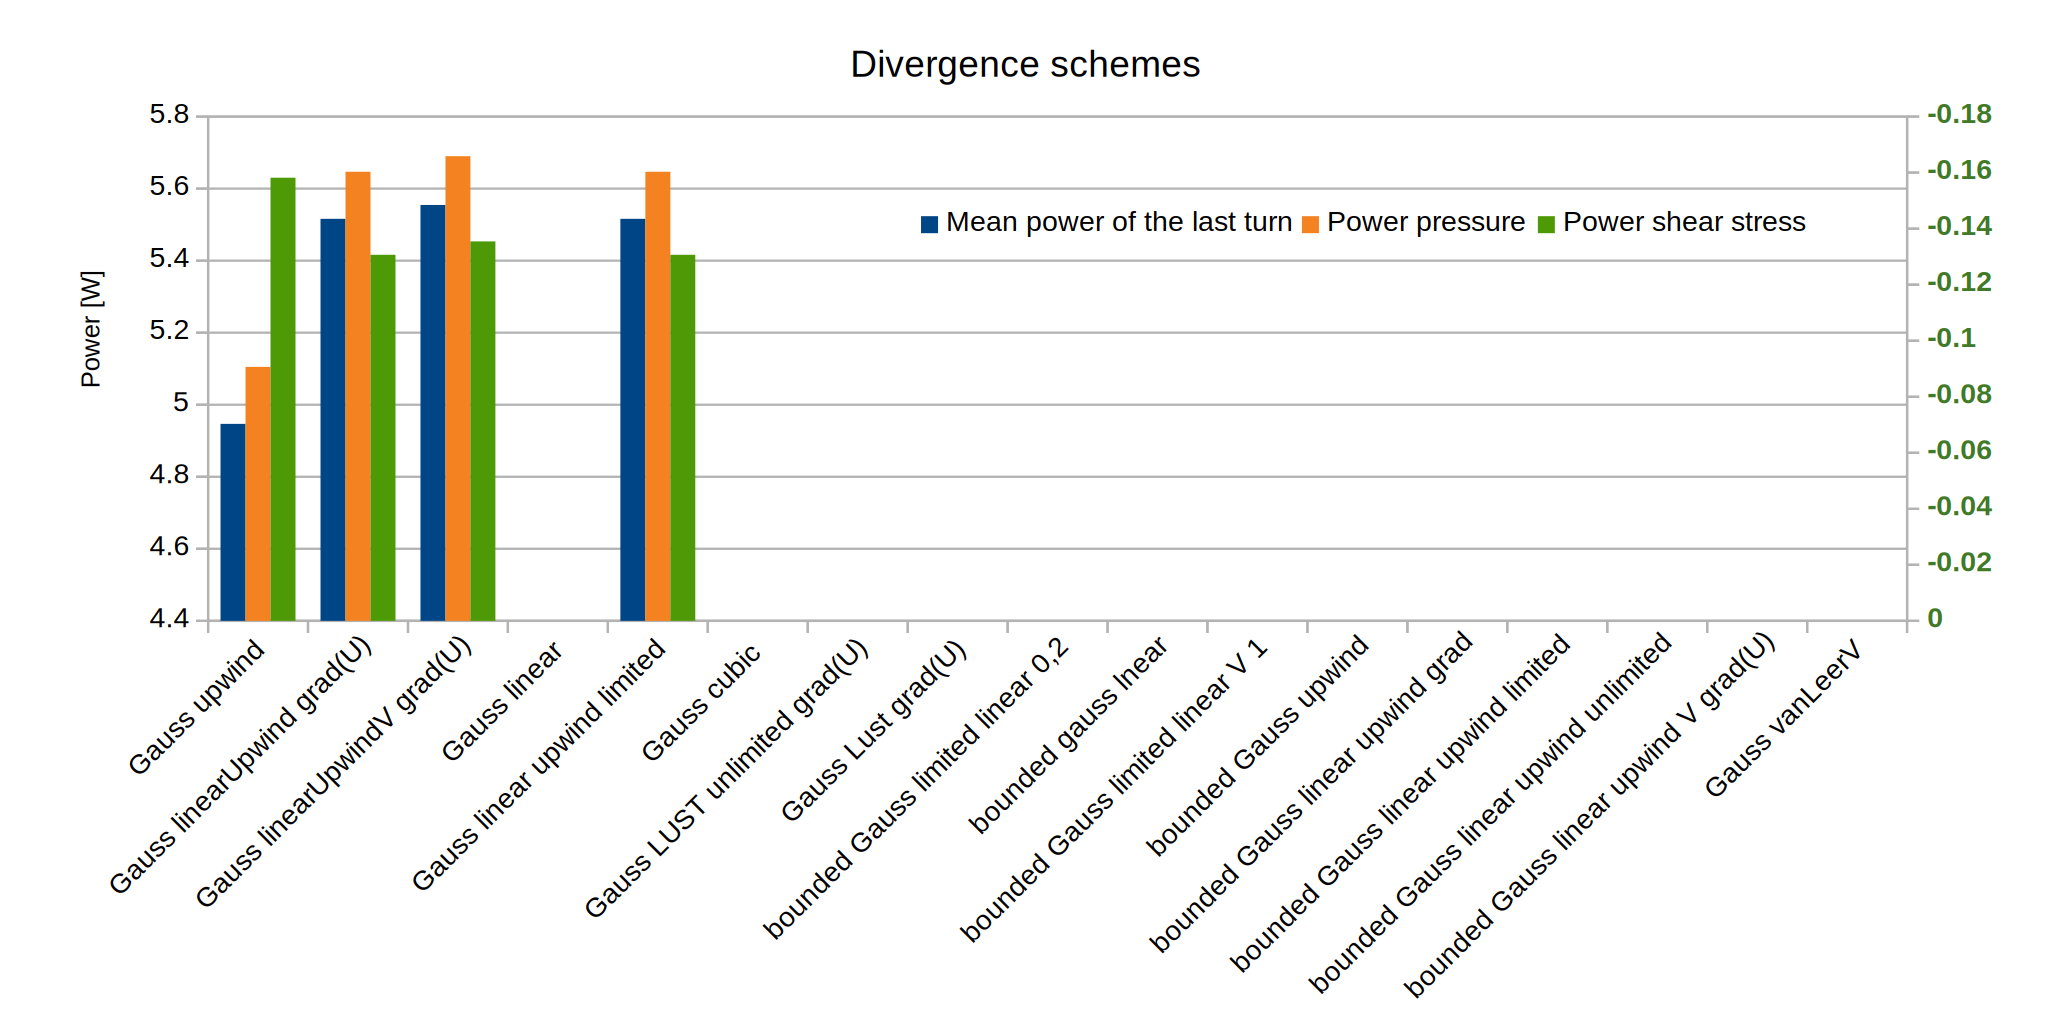
\includegraphics[height=7cm]{images/schemes/divschems-results.pdf}
\end{figure}
In this case as introduced before large number of schemes don't work. Considering the schemes which work properly, more remarcable difference can be detected.
The pressure power varies of 10\% in any case, and it is higher than simply upwind configuration. The power loss change for 20\% more and so overall power increases of 10\% reaching 5.5 W, similar for all schemes. Calculation time increases of 5\% for Gauss linearUpwind grad(U) while for the other decreases of 10\%. However some warning during calculation suggest to not trust at all the last two scheme, and for that section the Gauss linearUpwind grad(U) seems to be the more promising one. Residual are of the same order for all the scheme. However the "V" scheme is characterized by smoother behavior and less residual peacks iteration after iteration. %immagine per comparare?


\subsection{Laplacian schemes}
The laplacian operator act as follows:
\begin{equation}
\nabla^2 \bm{U} = \frac{\partial^2 U_x}{\partial x^2}+ \frac{\partial^2 U_y}{\partial y^2} + \frac{\partial^2 U_z}{\partial z^2}
\end{equation}

Typically it is associated to the diffusive term. Gauss scheme is the only one available and requires the interpolation scheme used and the normal gradient scheme, define in the proper subsection \textit{interpolationSchemes} and \textit{snGradSchemes}. Therefore the command would be:

\begin{center}
{\ttfamily laplacian	Gauss	<interpolationSchemes>		<snGradSchemes>}
\end{center}

Therefore as anticipated the effect of different gradient scheme, were tested in this section.

\paragraph{Results} \mbox{}\\
The different type of schemes are reported in the following figure.
\begin{figure}[H]
\centering
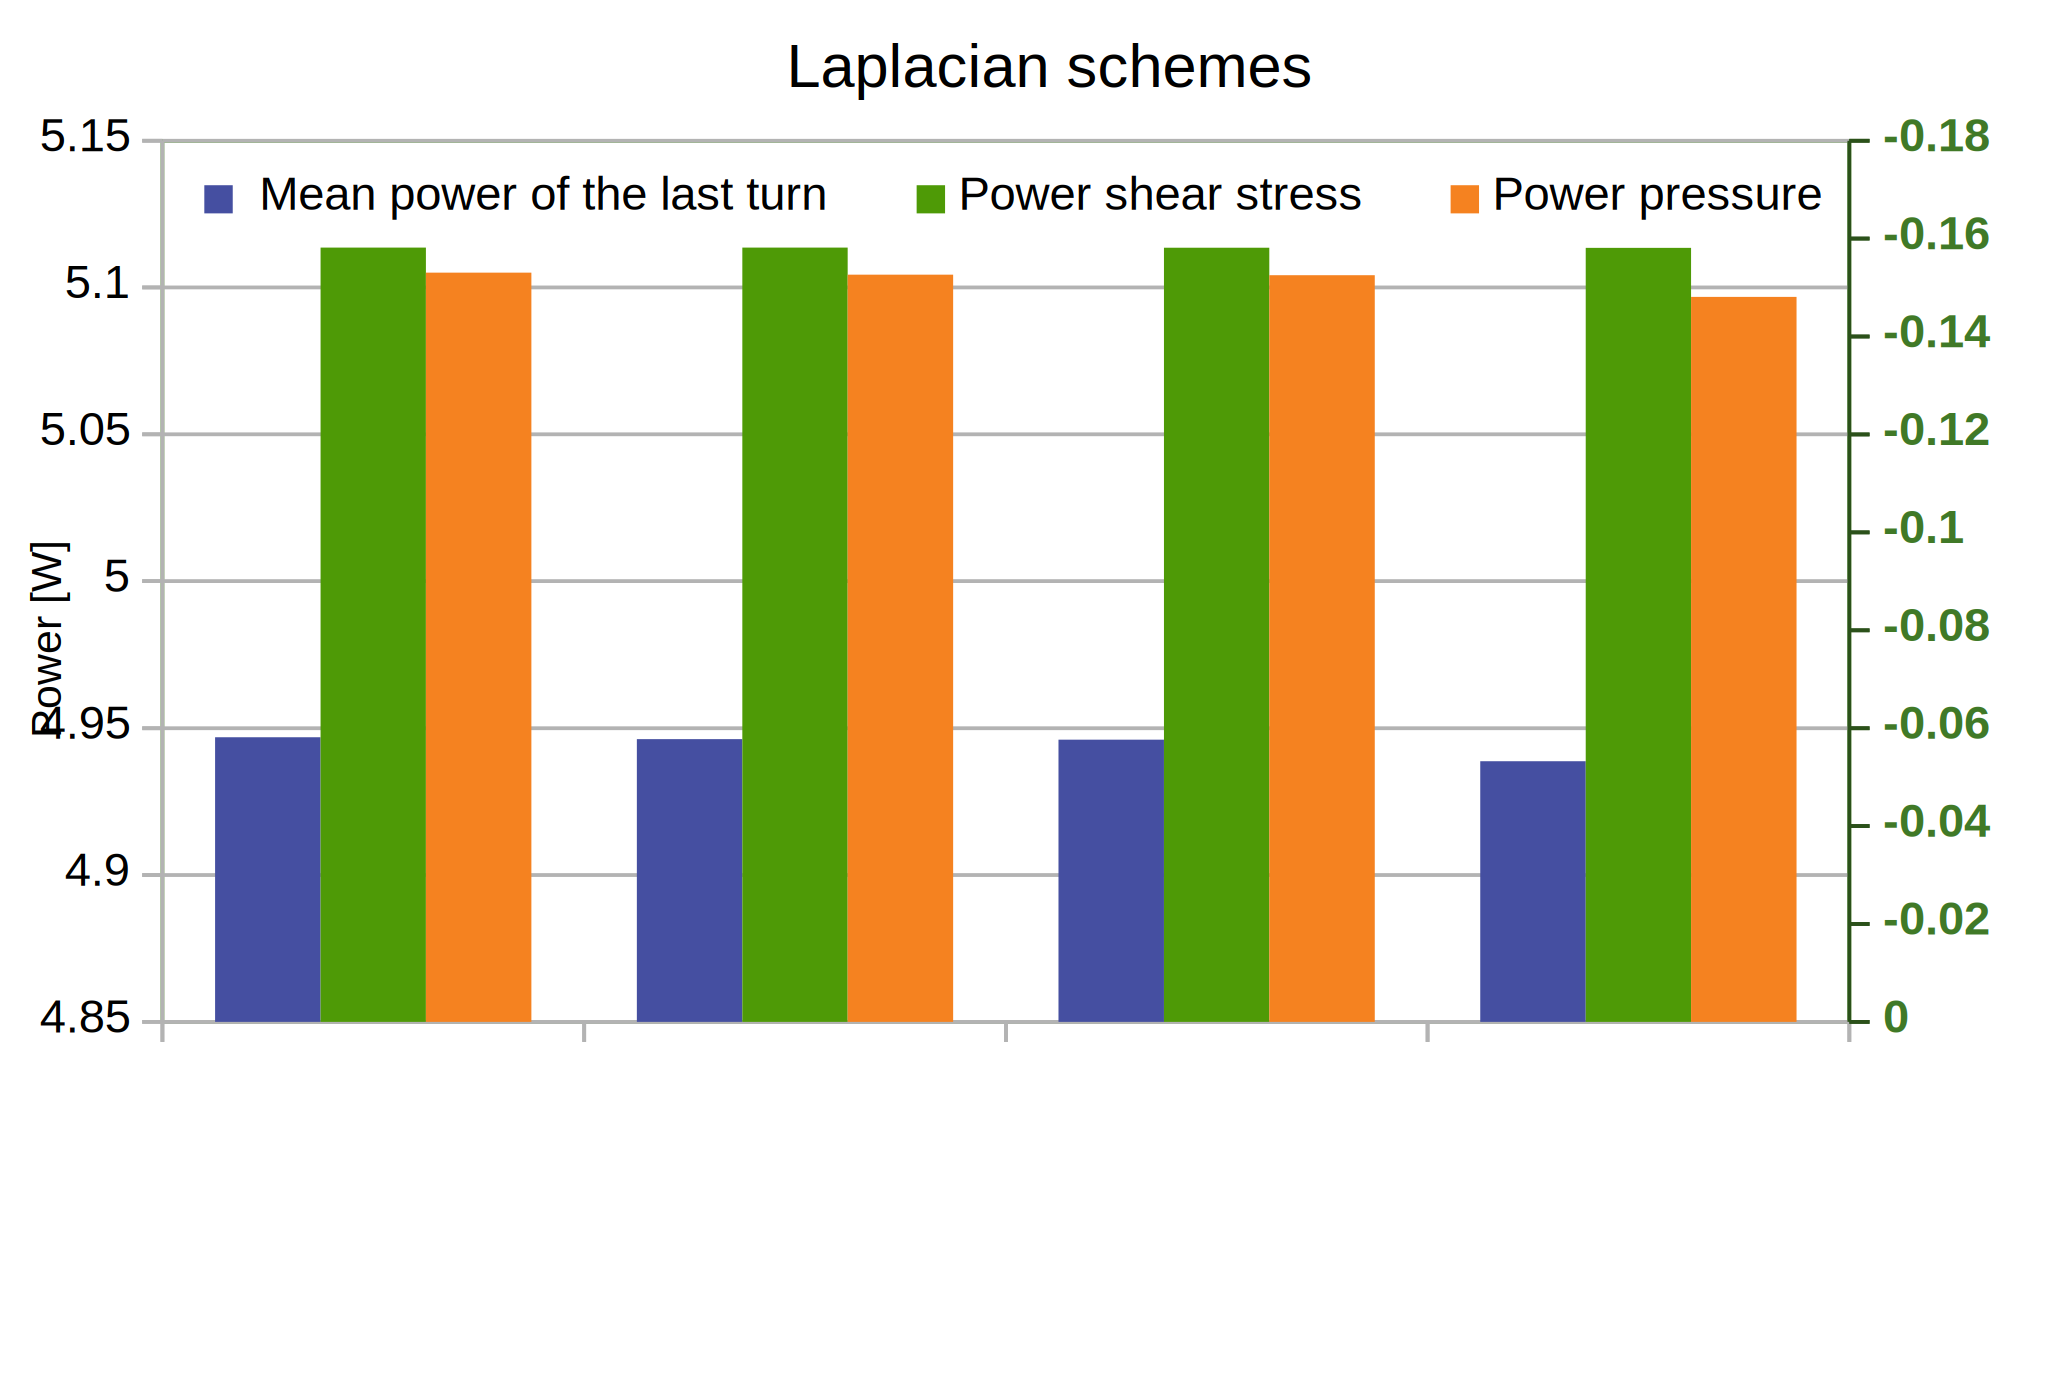
\includegraphics[height=6cm]{images/schemes/laplacianschems-results.pdf}
\end{figure}

Laplacian schemes are the only one scheme in which all what we tried works properly without errors or warning. The reference case is the most advanced one, so our attention was focus into unsterstand which is the impact of the non orthogonality correction. For what concern calculation time, the limited correction penalize the machine time (of 1.\%), with no difference in the calculated quantities (less than 0.5\%). Instead uncorrected scheme save more or less 40.\% of time, giving the same results with the same deviation of previous schemes. This could be an evidence of the fact that our mesh is able to guarantee that non orthogonality remain bounded. Residual are not characterized by sensible differences

\subsection{Conclusions}
Up to now, comparison has been made considering the integral mean power in the last turn.
However high order schemes can introduce numerical instability, no more dumped by the numerical diffusion of the lower order schemes. 
Therefore to judge the stability we have decided to look at the instant power. 
What is interesting is that, for gradient scheme as for laplacian scheme there is no difference. 
Since the time for the calculation is almost independent by the scheme, we move to the higher order:


\begin{tabular}{lcl}
\foam{laplacian} & \quad \quad &\foam{Gauss linear corrected} \\ 
\foam{grad}  & \quad \quad & \foam{Gauss cubic}
\end{tabular}

\begin{figure}[H]
\centering
\subfigure[Reference case]{\includegraphics[width=5.5cm]{{images/schemes/InstantPower_casobase}.png}}
\subfigure[Backward]{\includegraphics[width=5.5cm]{{images/schemes/InstantPower_backward}.png}}
\subfigure[Linear upwind]{\includegraphics[width=5.5cm]{{images/schemes/InstantPower_linearupwind}.png}}
\caption{Instantaneous power with difference schemes.}
\label{fig:schemes-instant-power}
\end{figure}

For what concern instant power there are some differences between backward and linear upwind compared to default settings.
\\
Some differences can be highlighted, as we can see in figure \ref{fig:schemes-instant-power}.


%%% inserisci immagini delle potenze istantanee

The fluctuation using backward scheme seems to be related to some turbulence phenomena, or lower frequency unstedy effects, like flow detachment. 
Instead for linear upwind schemes, the fluctuation is very high. 

From our point of view such fluctuation in power, for a 3 bladed machine seems strange. 
Power drops and rises suddently, therefore we consider that behavior as a result of numeric instability. 
In the end we have selected:


\begin{tabular}{lcl}
\foam{time} & \quad \quad & \foam{backward} \\ 
\foam{divergence} & \quad \quad & \foam{Gauss upwind}
\end{tabular}



%%%%%%%%%%%%%%%%%%%%%%%%%%%%%%%
%	from:
% https://www.openfoam.com/documentation/user-guide/fvSchemes.php#x23-870273
% https://cfd.direct/openfoam/user-guide/fvschemes/
% https://www.openfoam.com/documentation/cpp-guide/html/guide-schemes.html

\section{Solver parameters}

In OpenFoam the solver implemented to deal with incompressible transient problems with moving mesh is \foam{pimpleDyMFoam}.
This command is quite flexible since it can behave both as pimple and piso mode. 
Actually it allows to specify:
\begin{itemize}
\item number of outer correctors, typical of the Pimple algorithm;
\item number of inner correctors, typical of Piso algorithm;
\item number of non orthogonal correctors, for highly non orthogonal meshes.
\end{itemize}

In general Pimple is preferred when large time steps are suitable and when the pressure and velocity transient behavior is not of interest;
Piso instead is preferred when small time steps are imposed but the nature of the problem or when a precise transient analysis is required.

\begin{lstlisting}[language=c++, caption={\foam{pimpleFoam} source code extract.}]
// * * * * * * * * * * * * * * * * * * * * * * * * * * * * * * * * * * * //

    Info<< "\nStarting time loop\n" << endl;

    while (runTime.run())
    {
        #include "readTimeControls.H"
        #include "CourantNo.H"
        #include "setDeltaT.H"

        runTime++;

        Info<< "Time = " << runTime.timeName() << nl << endl;

        // --- Pressure-velocity PIMPLE corrector loop
        while (pimple.loop())
        {
            #include "UEqn.H"

            // --- Pressure corrector loop
            while (pimple.correct())
            {
                #include "pEqn.H"
            }

            if (pimple.turbCorr())
            {
                laminarTransport.correct();
                turbulence->correct();
            }
        }

        runTime.write();

        Info<< "ExecutionTime = " << runTime.elapsedCpuTime() << " s"
            << "  ClockTime = " << runTime.elapsedClockTime() << " s"
            << nl << endl;
    }

    Info<< "End\n" << endl;
\end{lstlisting}

As we can appreciate in the source code of the algorithm, for each inner corrector the pressure equation is solved.
For each outer corrector instead the momentum equation is solved once while the pressure equation is solved as many times as the inner corrector prescribes.

The choice of the hybridization of the two iterators in our case is suggested by the analysis of the residuals.

Comparing the residuals in figure \ref{fig:solver-residuals-bad} we immediatly notice that the critical quantity is, in terms of residuals, the pressure,
while the two components of the velocity show a much better residual trends, of orders of magnitude.

This explains why we have chosen to run the majority of our simulation with a modified version of the Piso algorithm. 
In fact a great number of inner correctors, as we can see from the source code, implies just the solution of the pressure equation many times, 
while the outer correctors also solve the velocity field.
Finally since our aim is to try to reduce pressure residuals we prefer to increase the number of inner correctors respect to the outer ones.
This brings us to choose 1 outer correctors and 20 inner correctors.
 
\begin{figure}[H]
\centering
\subfigure[Pimple 50 outer 1 inner]{\includegraphics[width=8.5cm]{{images/solver/residuals50-1}.png}}
\subfigure[Piso 1 outer 20 inner]{\includegraphics[width=8.5cm]{{images/solver/residuals1-20}.png}}
\caption{Residuals comparison bewteen standard Pimple and our Piso.}
\label{fig:solver-residuals-bad}
\end{figure}

Moreover a great advantage of this variant is that it allows us to increase the Courant number up to 50 which means that our timestep could be a lot bigger than the one with default Piso condition. 

A rough estimation of the improvement in computational effort is:
\begin{itemize}
\item 100 times faster due to higher Courant number from 0.5 to 50;
\item 10 times slower due to 20 iterations instead of 2 of the inner loop;
\end{itemize}
This lead to approximately a net speed improvement of 10 times. 

\section{Turbulence}
In order to further improve the model also the turbulence model has been investigated.
Different turbulence models have been used in calculation:

\begin{enumerate}
\item Laminar model
\item \kepsilon model
\item \komegasst model
\end{enumerate}

\paragraph{Remark on the used mesh}
The mesh which has been used is that outcoming from the mesh-sensitivity analisys.

\paragraph{Comparison criterion}
It is worth noting that the assestment on the turbulence model is carried out via the evaluation of the $y^+ $ parameter which is directly related on the mesh size near the walls and on the wall shear stress.
The mesh features are mantained fixed while turbulence models have ben investigated, i.e. the mesh clustering is not a parameter in the turbulence model assestment.


\subsection{Turbulence model}


\paragraph{Laminar}\mbox{}\\
As first option the laminar model has been used in order to have a comparison tool.
It must be clarified that the physical situation that is expected is that of a turbulent motion, since the flow in evolving within a rotating blade domain; moreover the flow develops around aerodynamic profile on a wide range of angles of attach; at the end of the day what is expected is a vortical/turbulent-induced flow.
 

\begin{figure}[H]
\centering
\subfigure[Total pressure]{\includegraphics[width=8.5cm]{images/turbulence/laminar_pressureDrop.png}}
\subfigure[Drag wake zone]{\includegraphics[width=8.5cm]{images/turbulence/recirculation_scalarScaledGOODresolution.png}}
\end{figure}


\paragraph{$\bm{k}-\bm{\varepsilon}$ model}  \mbox{}\\
As first attempt for turbulence model the \kepsilon model has been used.
The result has been assessed in term of the $y^+ $ which is computed by OpenFoam on the patch of type \foam{wall}, namely \foam{lowerwall}, \foam{blade0}, \foam{blade1} and \foam{blade2}.
If the values of $y^+ $ would satisfy the condition:
\begin{equation}
y^+ > 30
\end{equation}

Then the turbulence model would be validated; this would mean that the solver is going to solve the $k-equation $ and $\varepsilon-equation $ in the far wake region without problems of singularity and, then, take advantage ofthe wall-functions at the wall to calculate the flow field.\\
The results are presented in the following table in terms of minimum and maximum $y^+ $ for each wall at the last timestep $t = 2.4[s]$.
\begin{table}[H]
\centering
\begin{tabular}{rcc}
\toprule
           & $min(y^+) $          & $max(y^+) $  \\ \midrule
lower wall & 6.793848e-01         & 4.095234e+00 \\
blade0     & $\round{5.503802e-02}$ & 7.997351e-01 \\
blade1     & 4.869300e-02         & 1.742530e-01 \\
blade2     & 7.257931e-02         & 7.748824e-01 \\ \bottomrule
\end{tabular}
\caption{Min and max $y^+$ values on the walls}
\label{table:turbolence-yplus}
\end{table}
As can be seen in table \ref{table:turbolence-yplus} the $y^+$ values do not allows us the choice of the \kepsilon turbulence model.

\paragraph{$\bm{k}-\bm{\omega} $ SST model}  \mbox{}\\
Given the $y^+$ values, is evident that the mesh clustering near the walls of the blades is suitable for the \komegasst model which avoids problems of singularity of the equations and can solve directly the boundary layers of the blades.\\
Particular attention has been paid for the mesh clustering in the O-grid near the wall of the blade, it has been set properly in order to guarantee the smooth variation of flow property from the BL to the free stream.

\subsubsection{Turbulence models comparison}
A brief qualitative comparative study of the performance of the machine, given different turbulence models has been carried out.

\paragraph{Mean power}
the mean power has been compared in the last turn starting at $t=1.8\s$ for all the three turbulence setups. 
As we can notice in figure \ref{fig:turbolence-powercomparison} the laminar model predict the highest power while the \kepsilon model prediction is the lowest.

\begin{figure}[H]
\centering
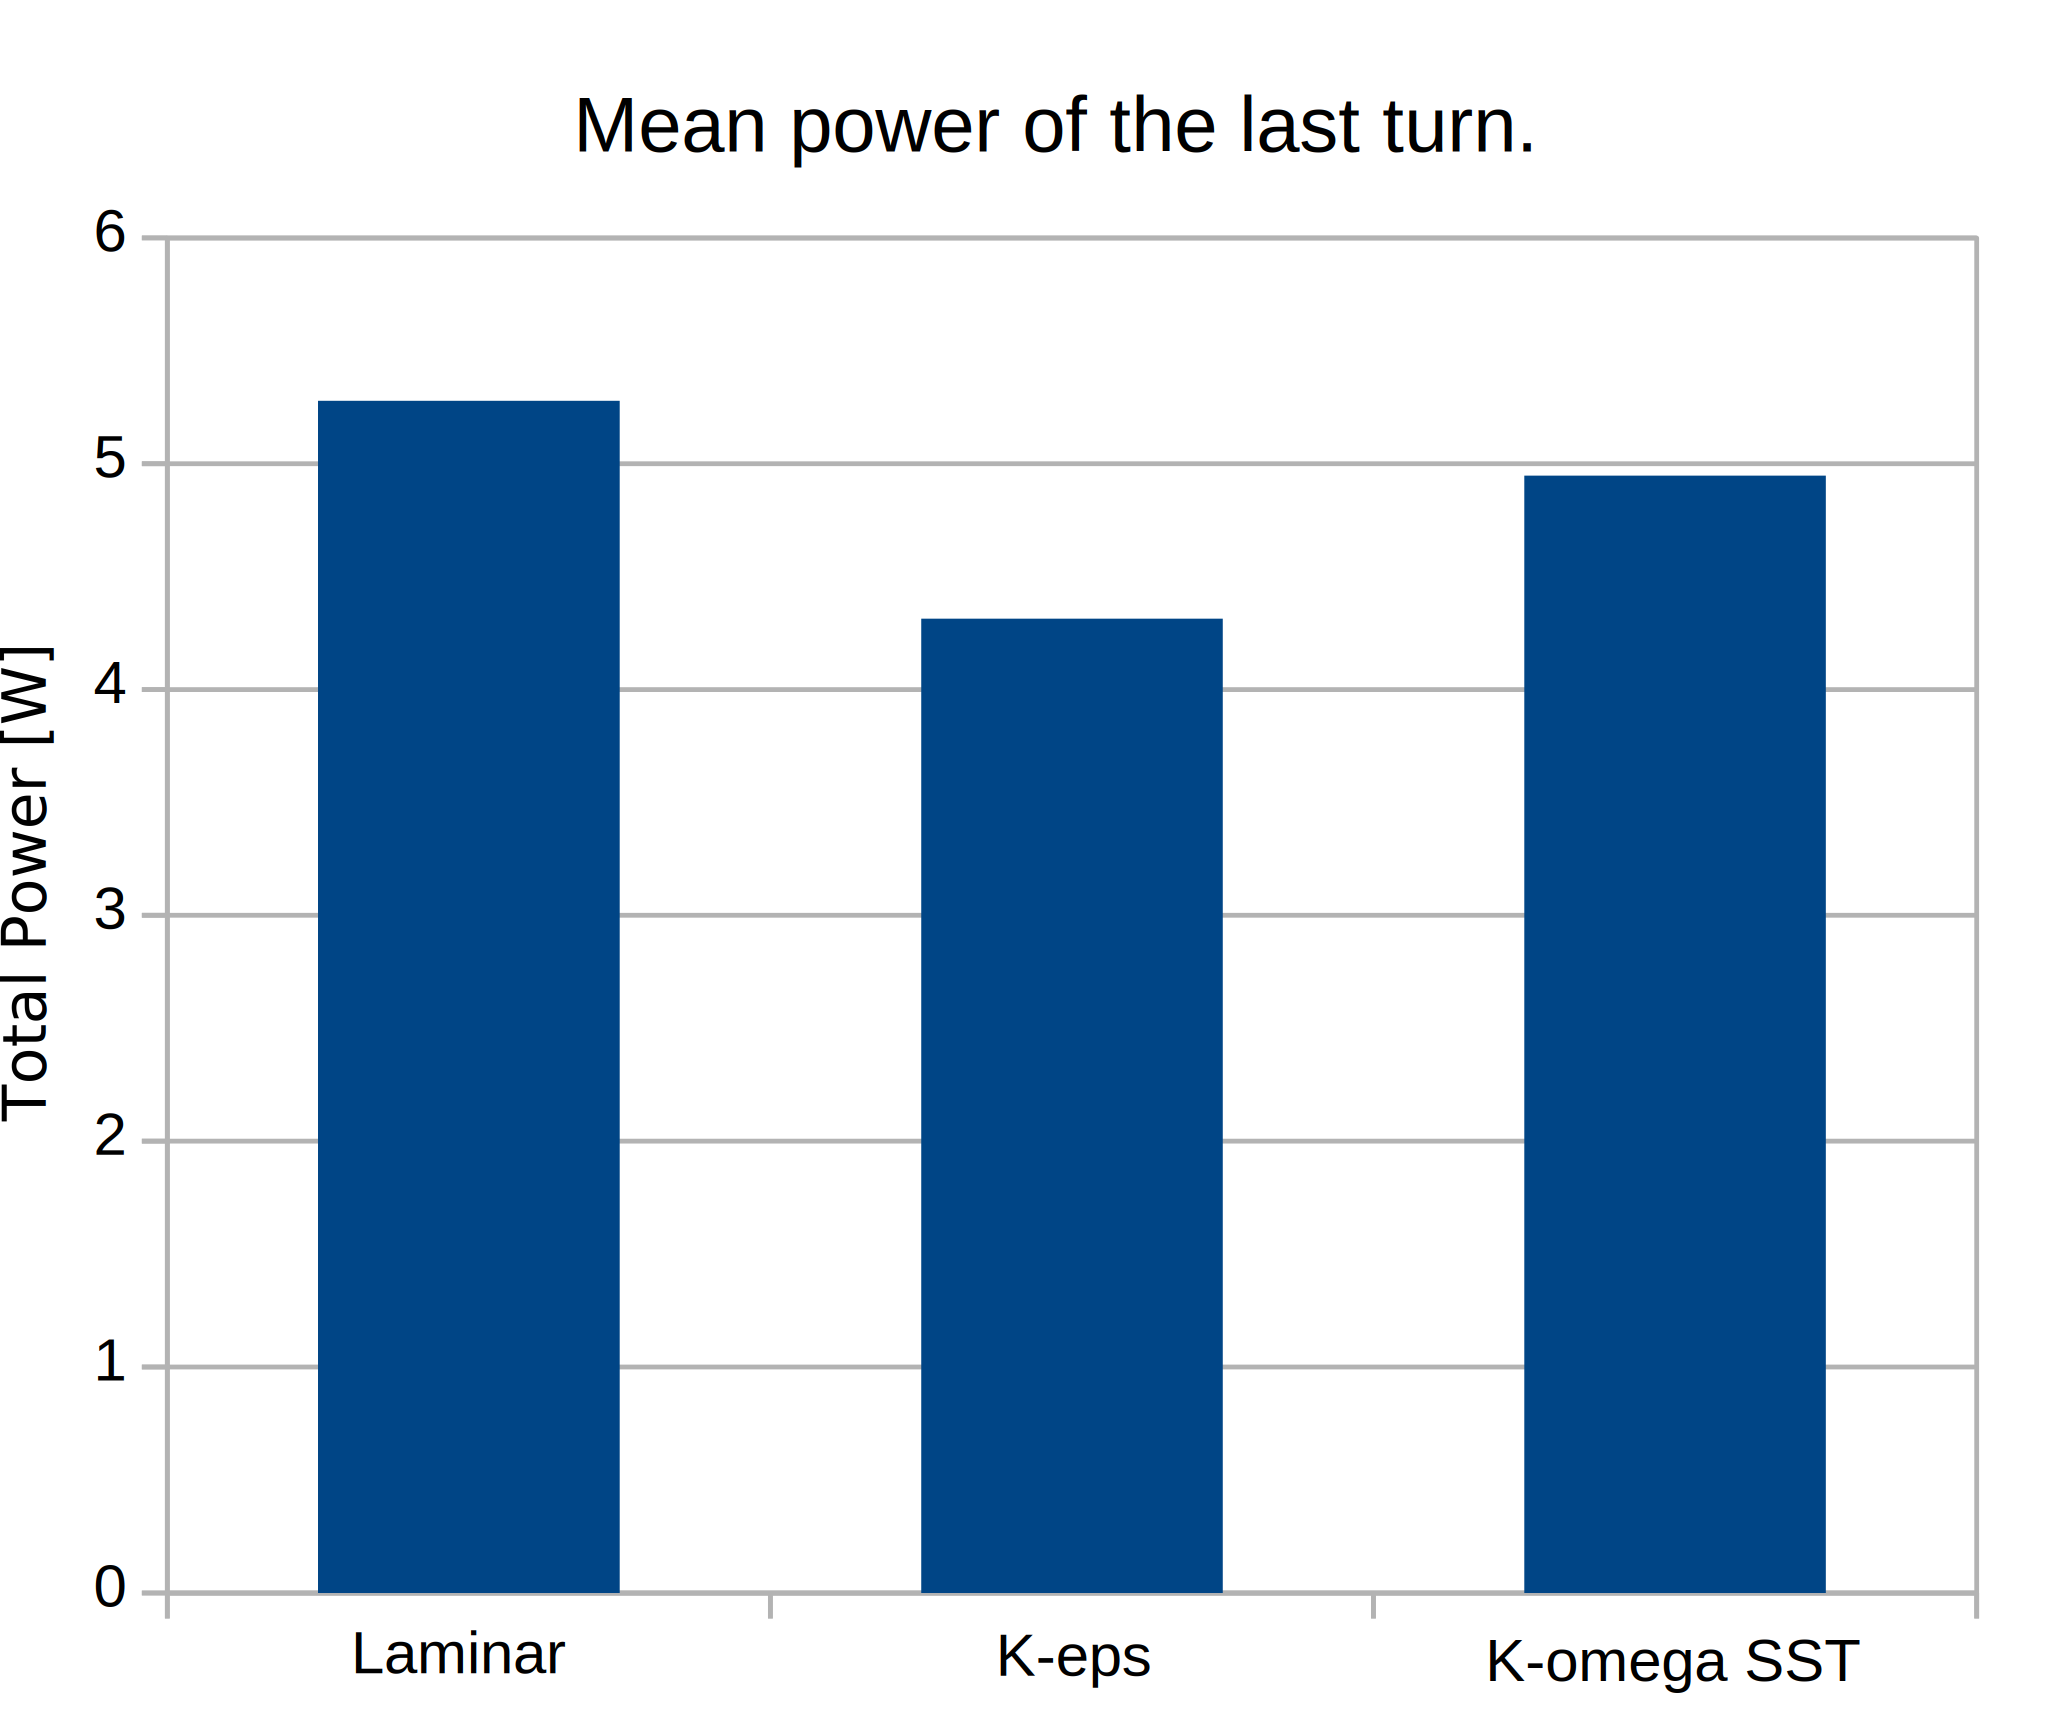
\includegraphics[width=8cm]{images/turbulence/MeanPower_comparison.pdf} 
\caption{Power comparison}
\label{fig:turbolence-powercomparison}
\centering
\end{figure}



\paragraph{Velocity profiles}
As first, a qualitative velocity profiles comparison has been performed in the wake regions,
where the effect of the turbulence is expected to play its major role.
The inspected regions are the following:
\begin{figure}[H]
\centering
\subfigure[First section zone: drag wake zone]{\includegraphics[width=8.5cm]{images/turbulence/VerticalBladeWake_screenshot.png}}
\subfigure[Second section zone: mean wake zone]{\includegraphics[width=8.5cm]{images/turbulence/LargeWakeScreenshot.png}}
\end{figure}

\begin{figure}[H]
\centering
\subfigure[Velocity profile - drag-zone wake]{
\label{fig:turbolence-bladewake-results}
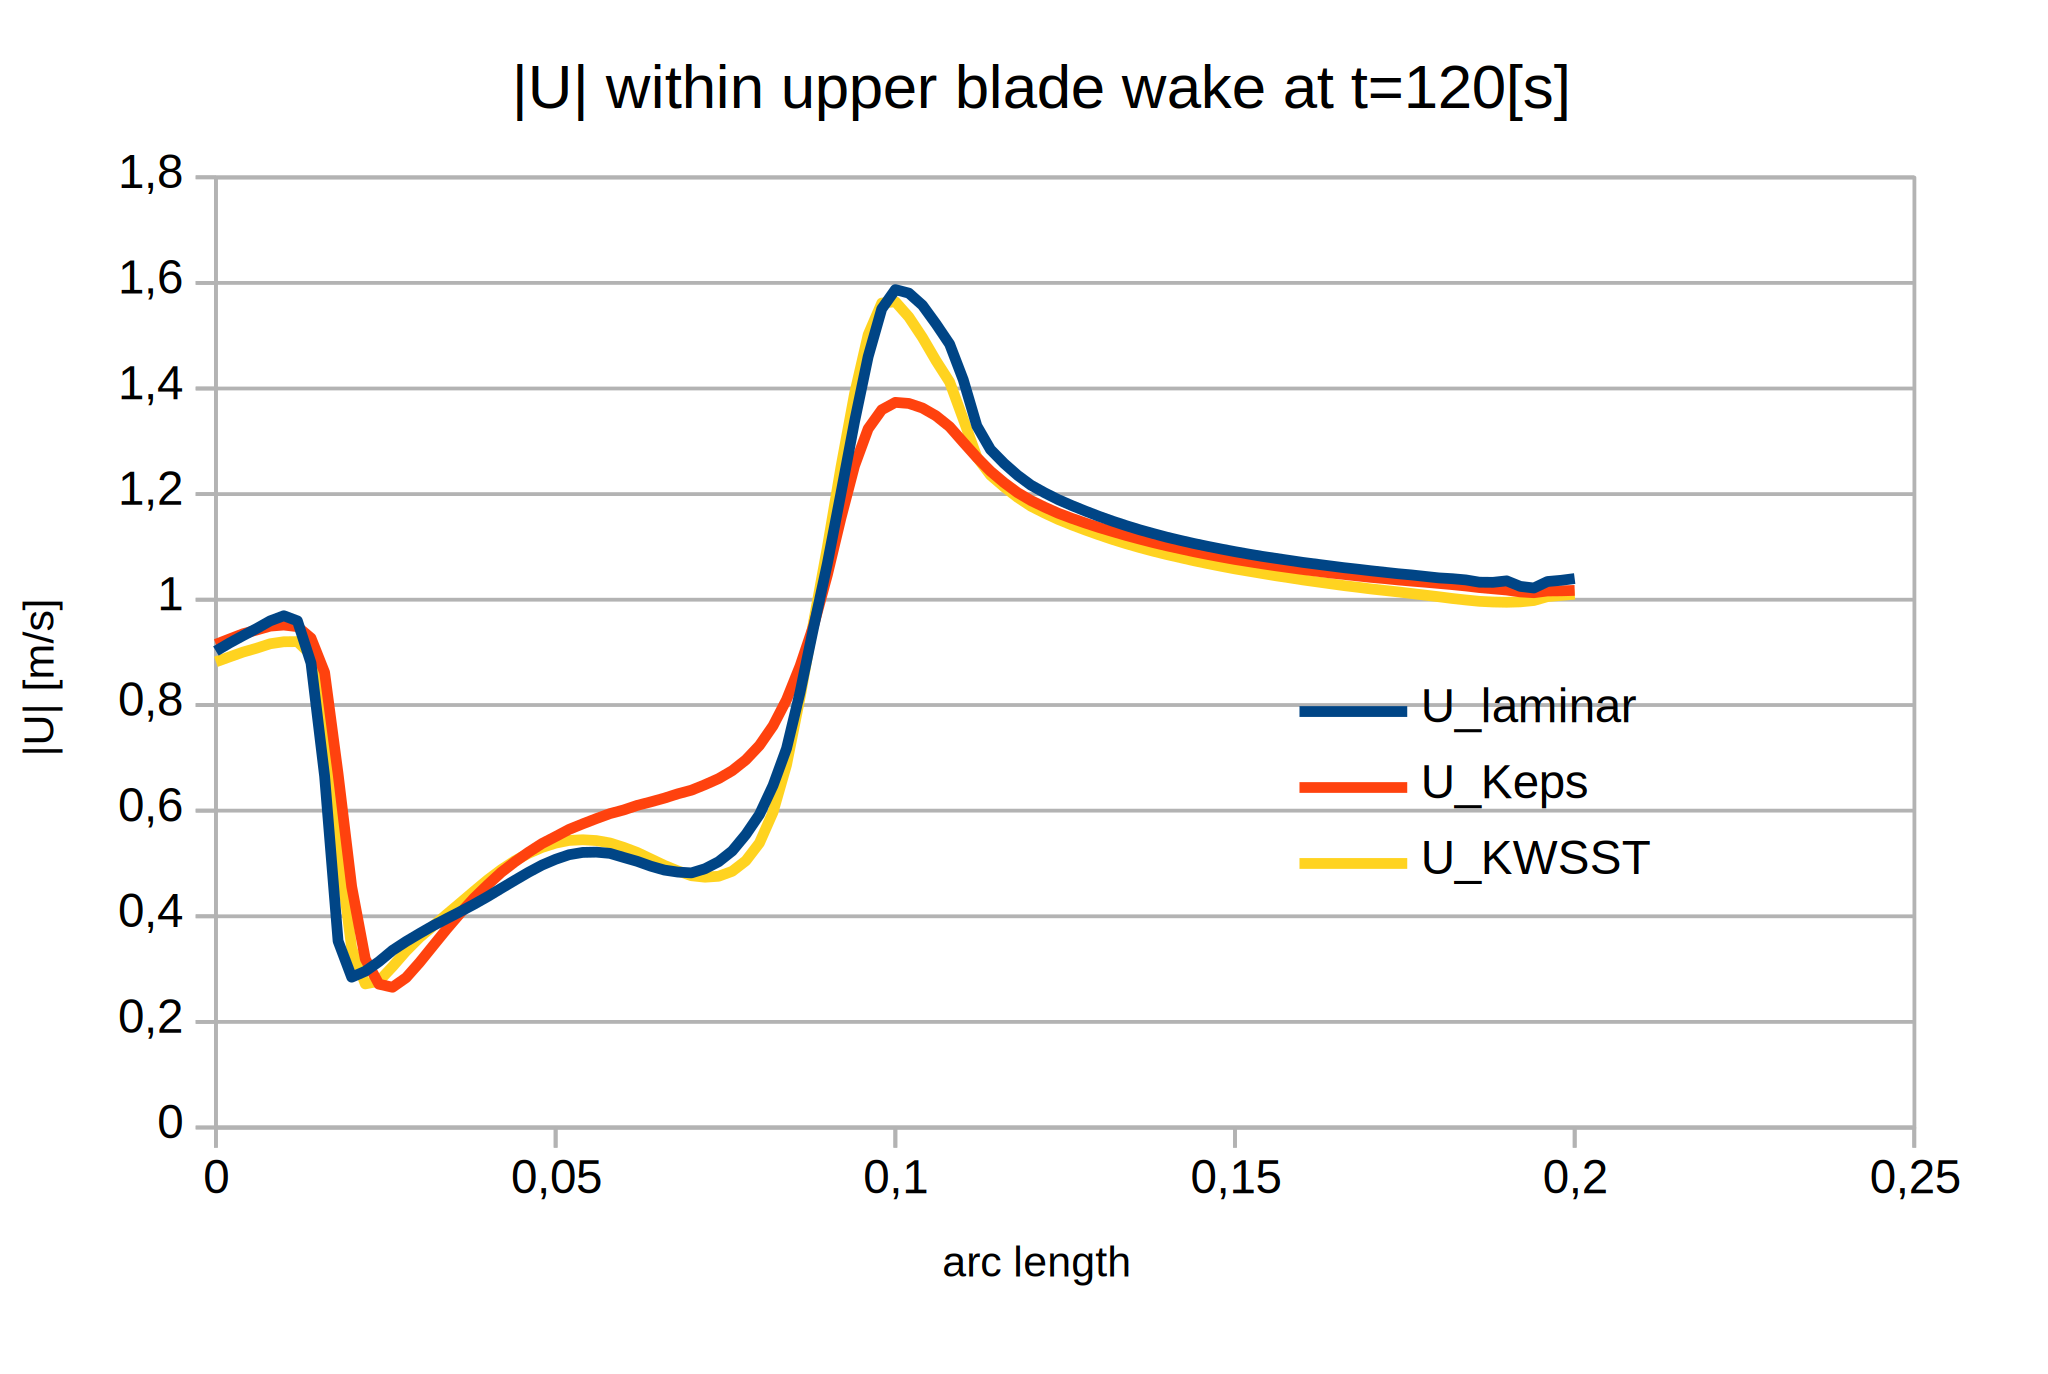
\includegraphics[width=8.5cm]{images/turbulence/UpperbladeWake.pdf}}
\subfigure[Velocity profile - mean-zone wake]{
\label{fig:turbolence-mainwake-results}
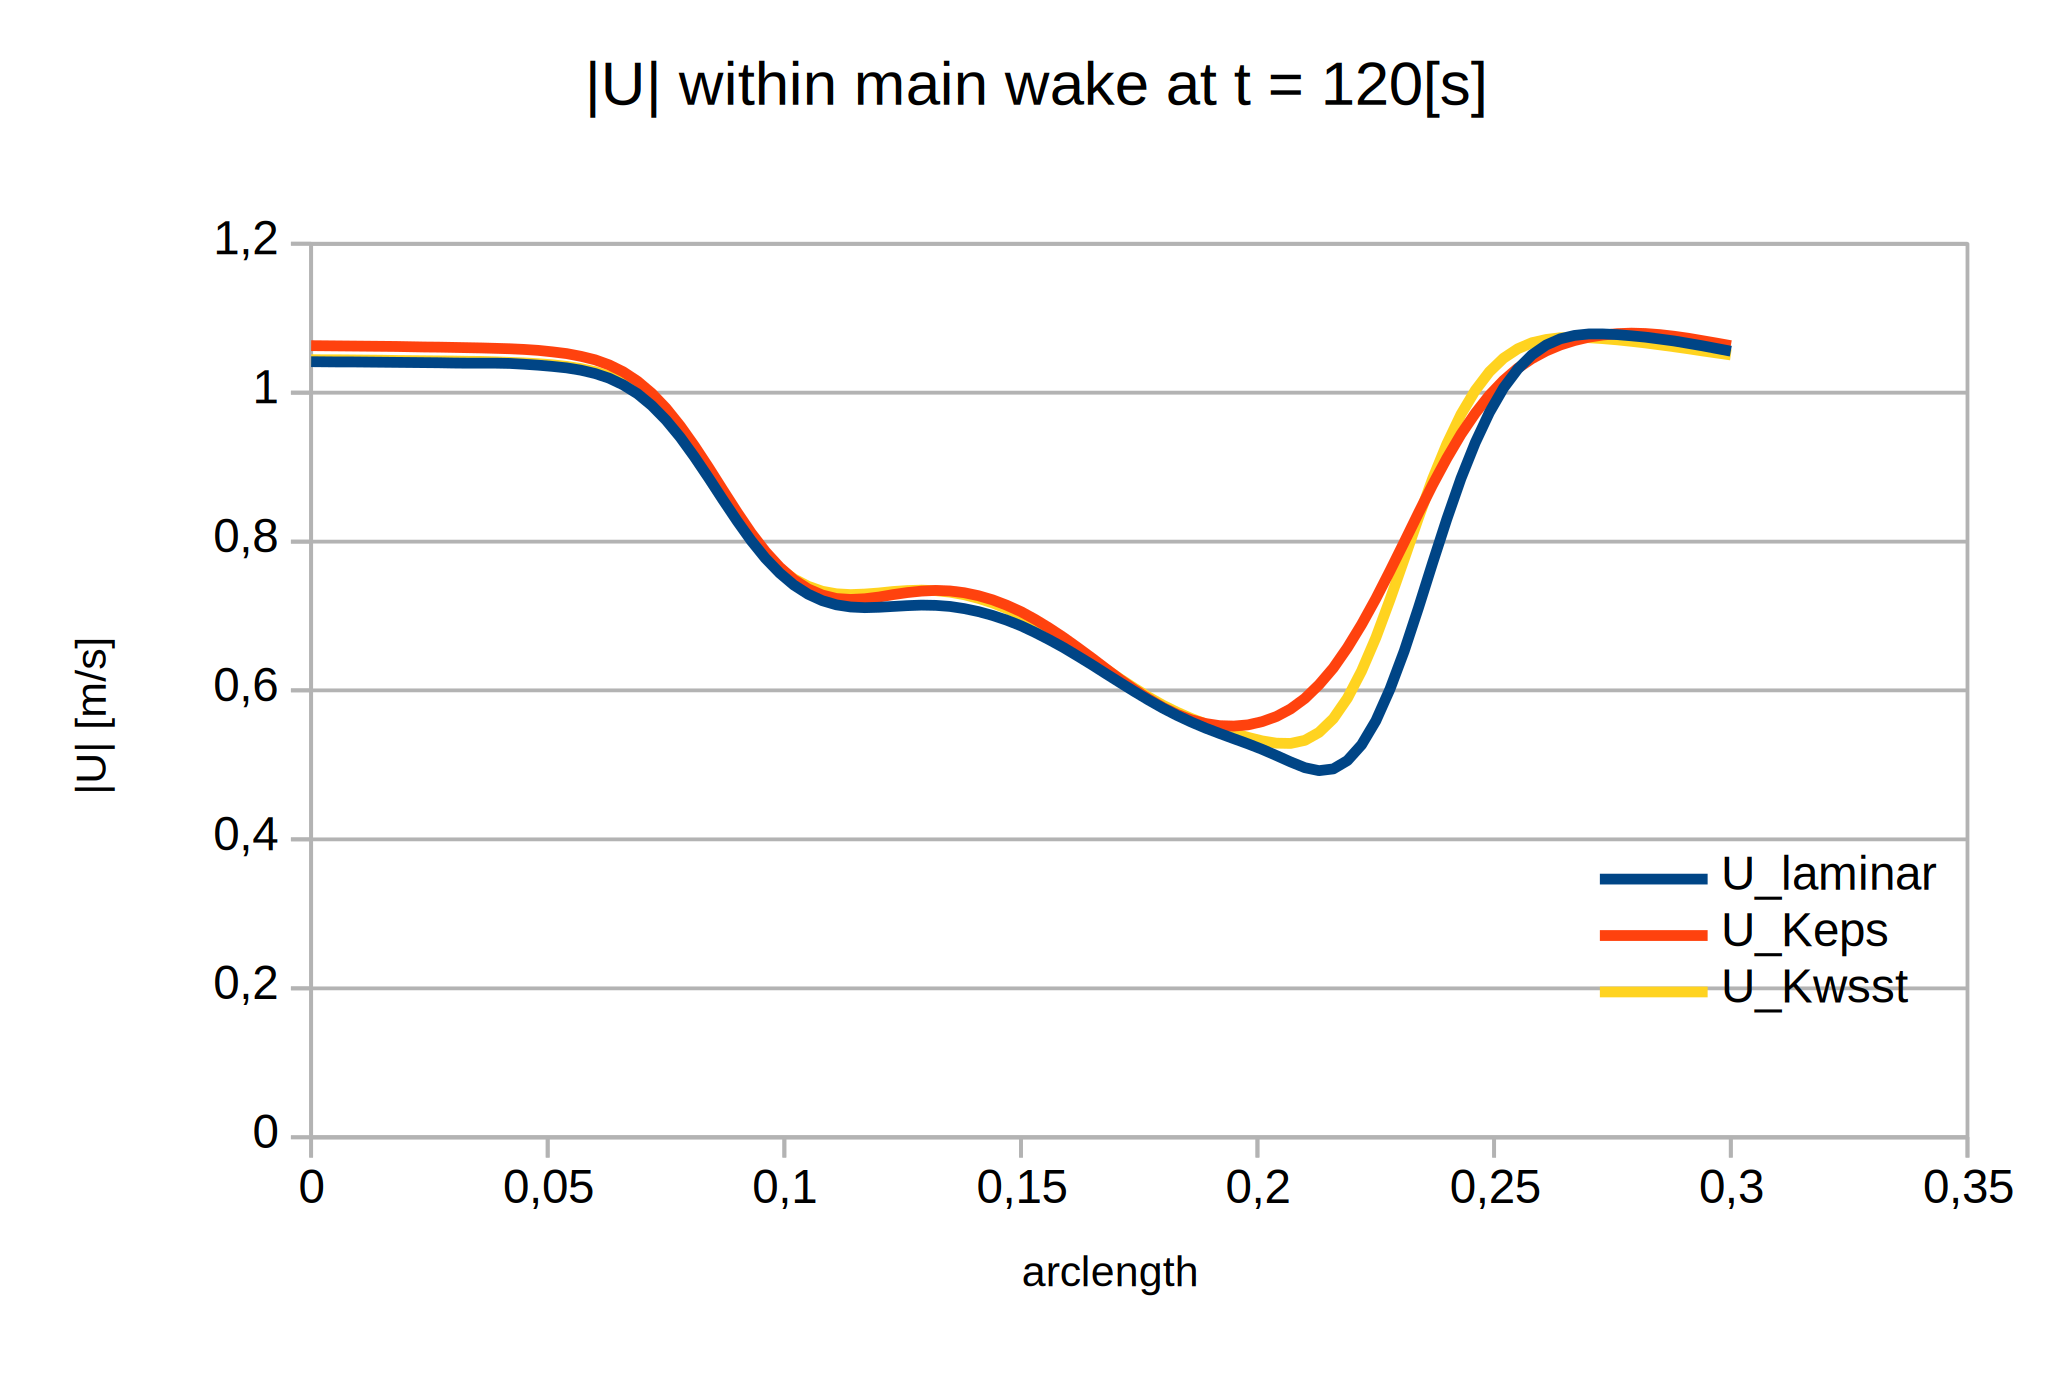
\includegraphics[width=8.5cm]{images/turbulence/U_mag_MainWake.pdf}}
\caption{Velocity profiles on different lines.}
\end{figure}

\subparagraph{Drag region wake}
First of all, it has to be noted that, on the first velocity section, the \kepsilon profile results in a different velocity profile with respect to the profiles outcoming from the laminar and \komegasst models which, instead, have been observed to be quite similar.
The \kepsilon profile appears to smear out the velocity gradients which are supposed to be magnified in the viscosity-dominated wake regions.
Results are represented in figure \ref{fig:turbolence-bladewake-results}
%\begin{figure}[H]
%\centering
%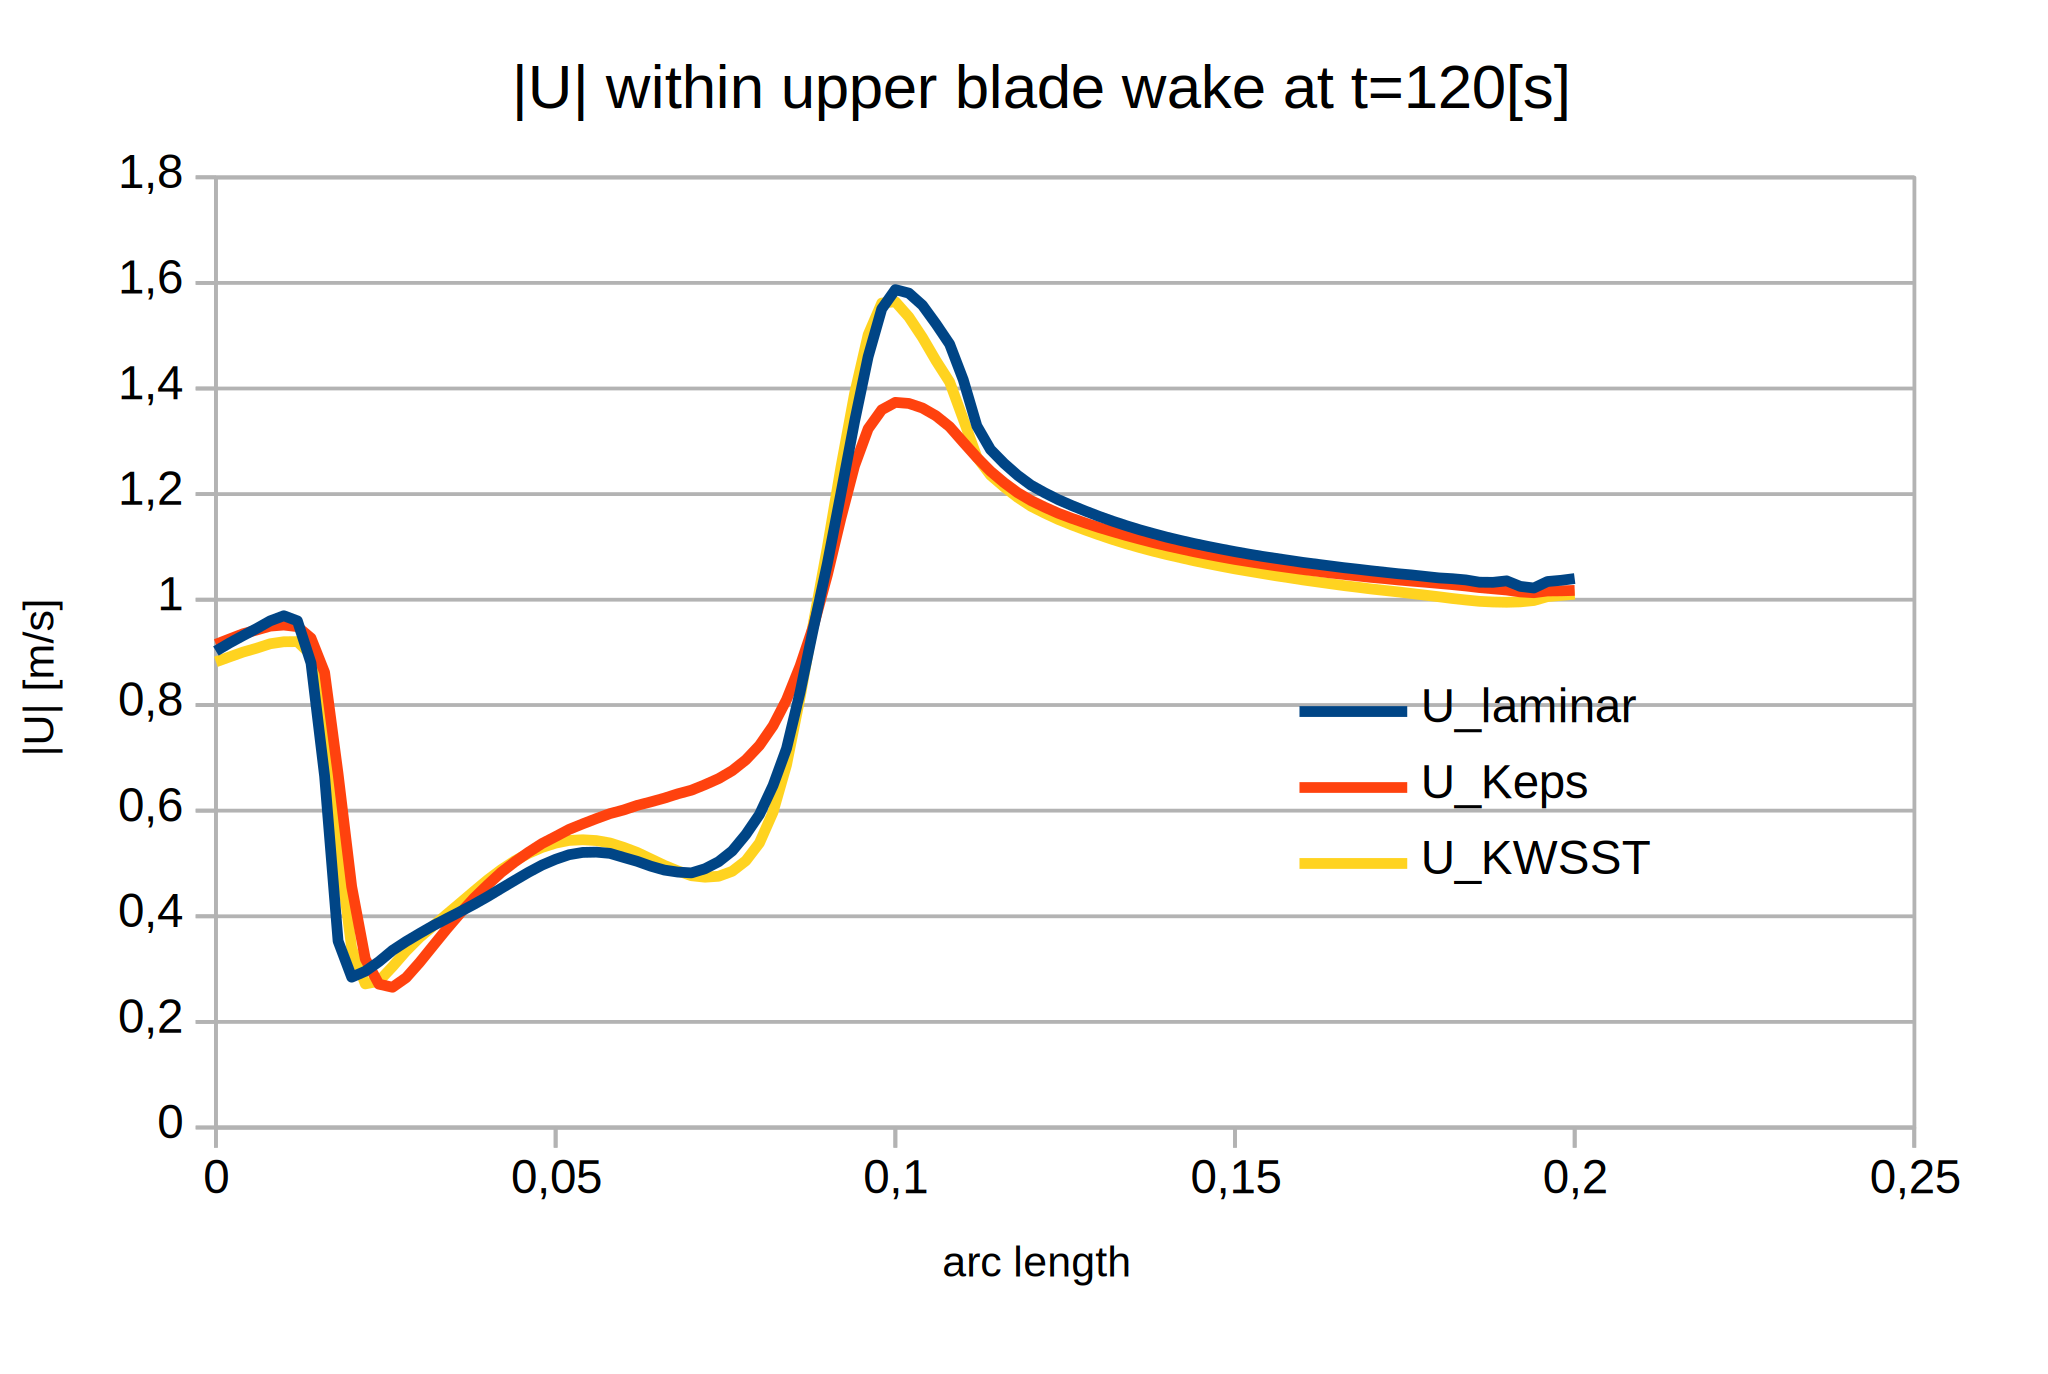
\includegraphics[width=10cm]{images/turbulence/UpperbladeWake.pdf} 
%\caption{Velocity profile on the drag-zone wake of the blade}
%\centering
%\end{figure}

\subparagraph{Large wake region}
On the largest wake section it can be noted again that the difference between velocity profiles is not negligible, in this case it is worth noting that the laminar simulation is that featured by the largest flow deceleration with respect to the upstream profile; this fact could explain the largest mean power extraction that has been found before fo the laminar case.
Results are represented in figure \ref{fig:turbolence-mainwake-results}

%\begin{figure}[H]
%\centering
%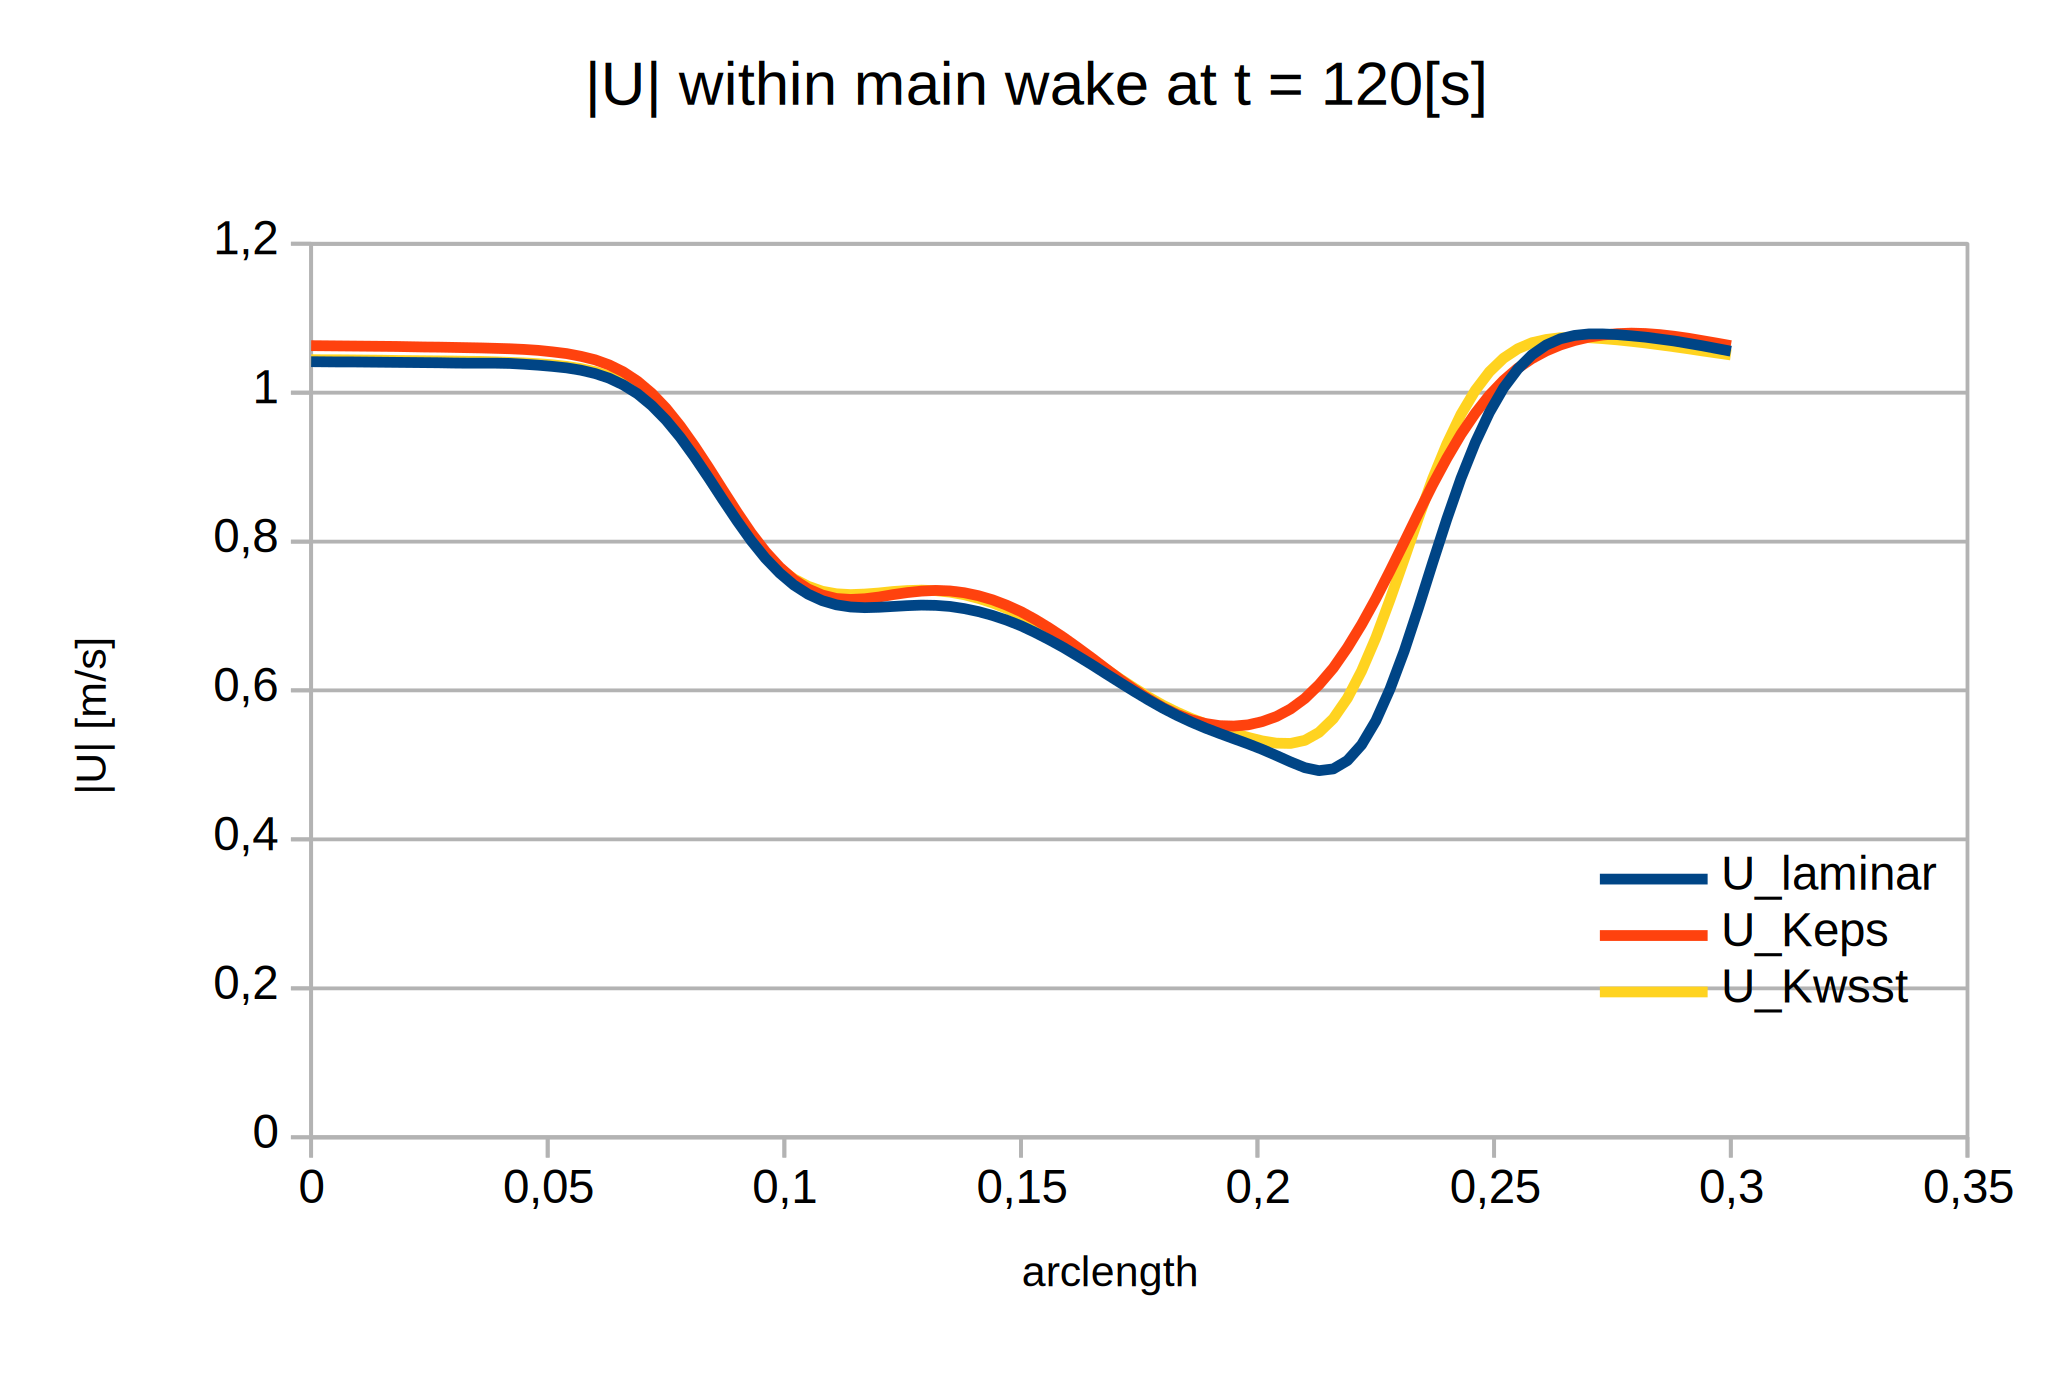
\includegraphics[width=14cm]{images/turbulence/U_mag_MainWake.pdf} 
%\caption{Velocity profile on the drag-zone wake of the blade}
%\centering
%\end{figure}

\subparagraph{Remarks}
From a qualitative point of view it is important to stress the fact that a great accordance has been found between the results of the laminar and the \komegasst simulation and instead the \kepsilon simulation does not follow the other velocity profiles neither qualitatively.

\subparagraph{Boundary layer}
In order to further clarify this situation, another inspection has been done: the boundary layer on a blade.
The profile has been explored at the time $t=115\s$, in correspondance of a null angle of attack of the lower blade with respect to the incoming flow.
Great attention has been paid on the extention of the plot stencil to end within the refinement region.


\begin{figure}[H]
\centering
\includegraphics[width=8cm]{images/turbulence/BL_LowerBlade_screenshot.png} 
\caption{Velocity profile on the drag-zone wake of the blade}
\centering
\end{figure}

The velocity profiles only for the \komegasst and \kepsilon have been compared.


\begin{figure}[H]
\centering
\subfigure[Velocity profile - drag-zone wake]{
\label{fig:turbolence-bladewake-results}
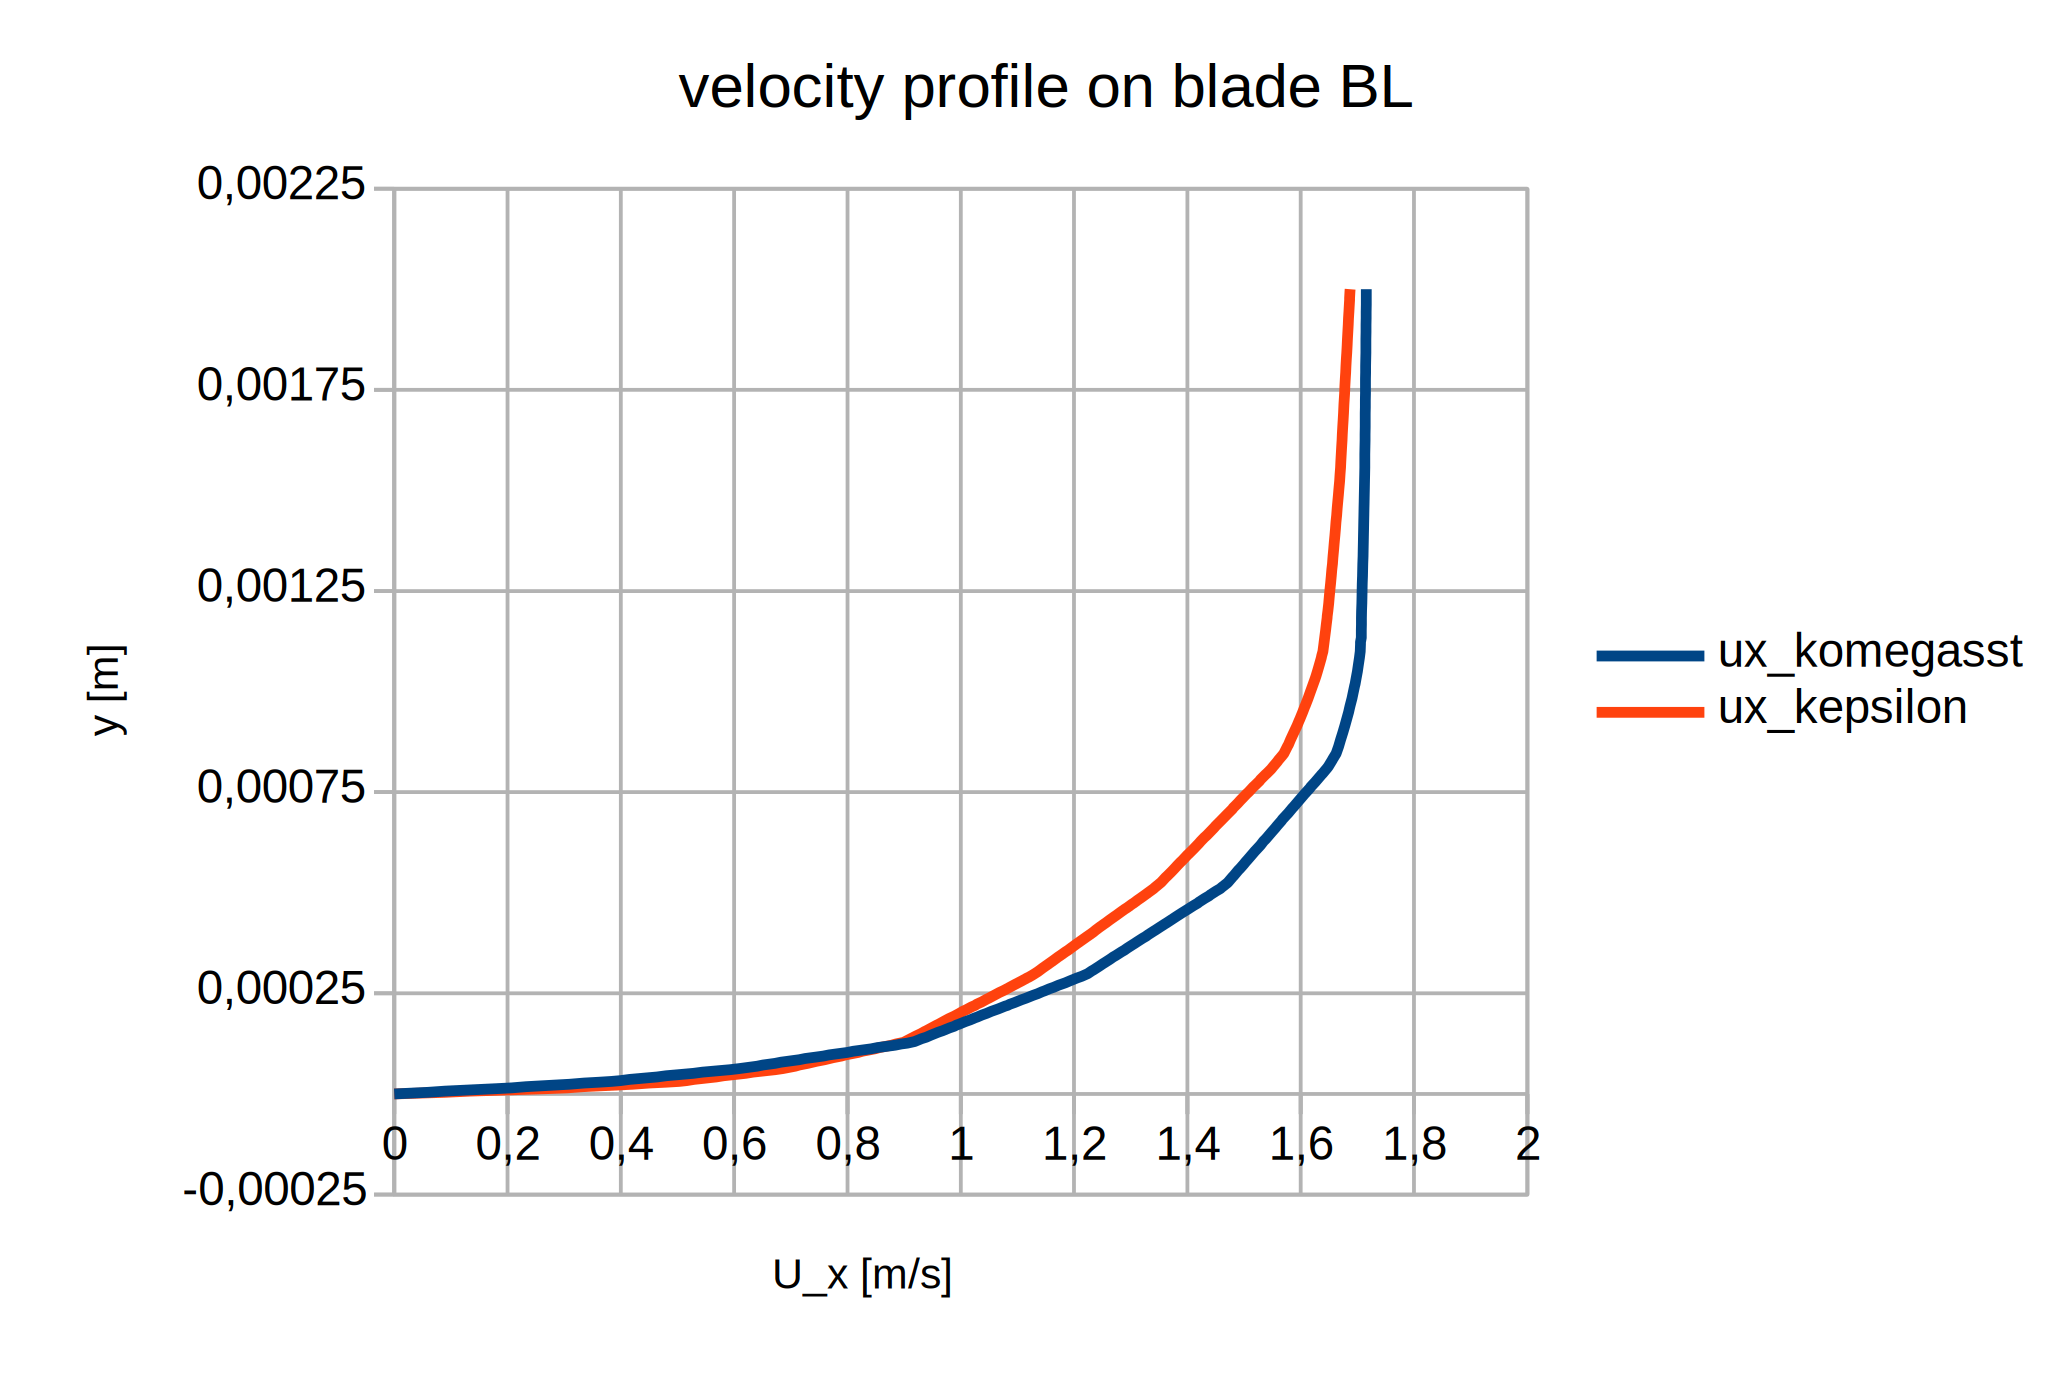
\includegraphics[width=8.5cm]{images/turbulence/detailBL_kW_Keps.pdf}}
\subfigure[Velocity profile - boundary layer.]{
\label{fig:turbolence-mainwake-results}
\includegraphics[width=8.5cm]{images/turbulence/kWsst_BL_sublayer.pdf}}
\caption{Velocity profiles - $\text{U}^+$ respect to $y^+$.}
\end{figure}

%\begin{figure}[H]
%\centering
%\includegraphics[width=14cm]{images/turbulence/detailBL_kW_Keps.pdf} 
%\caption{Velocity profile on the drag-zone wake of the blade}
%\centering
%\end{figure}

The velocity profiles obtained remark the discrepancy between velocity profiles from the different models.

Then a nondimensional analysis has been carried out on the boundary layer approximation of the \komegasst turbulence model.

%\begin{figure}[H]
%\centering
%\includegraphics[width=14cm]{images/turbulence/kWsst_BL_sublayer.pdf} 
%\caption{Velocity profile on the drag-zone wake of the blade}
%\centering
%\end{figure}

%From the previous results it can be observed that the BL velocity distribution in the linear region is quite different from that developed theoretically for simple shear flow under the assumption of large Reynolds number i.e. thin boundary layer on flat plate.
%This trend could probably be justified considering that this particular type of flow displays low Reynolds number which turns out into low turbulence effects.
%Only a comparison with experimental results could fully clarify this situation.
%The previous hypothesis found its root in the observation of the resemblance of laminar and \komegasst velocity profiles.\\
%\todo{} PROBABILE STRONZATA

\subsection{Flow detatchment}

As previously mentioned, this kind of machine exploit an incompressible flow, evolving within aerodynamic profiles with varying angles of attach.
It is straightforward that a good capture of flow detatchment and recirculation are of primary importance.
The \kepsilon turbulent model is not suited for capturing the flow detatchment.
The \komegasst turbulence model, coupled with a proper refinement strategy near the walls is capable of reproducing the flow detatchment and eventual subsequent recirculation
\begin{figure}
\includegraphics[width=8.5cm]{images/turbulence/recirculation_scalarScaled.png}
\includegraphics[width=8.5cm]{images/turbulence/recirculation_scalarScaledGOODresolution.png}  
\end{figure}

\begin{figure}
\includegraphics[width=8.5cm]{images/turbulence/recirculation_scalarScaledMESH.png}
\includegraphics[width=8.5cm]{images/turbulence/recirculation_vectorScaled.png}  
\end{figure}





\subsection{Turbolence intensity}
The turbolence intensity up to now is a parameter that was simple set to reasonable value. We have taken $5\%$ as turbolence intensity at the inlet and then we have evaluated the turbolent kinetic energy from that returning us the value for the initial value and the value at boundaries.
\begin{equation}
\label{eq:turbolent_I}
\text{turbolent intensity } \text{I} = \dfrac{u'}{U} = 0.05 = 5\%
\end{equation}
\begin{equation}
\text{turbolent kinetic energy } k = \dfrac{1}{2} \, \left( u'^2+v'^2+w'^2 \right) \approx \dfrac{3}{2} \, u'^2 = \dfrac{3}{2} \, \left(I\, \text{U} \right) ^2 = 0.00375 \m^2 / \s^2
\label{eq:turbolent_k}
\end{equation}

Since this value is obtained by common sense, we have tried to see how results would have changed with different turbolent intensities.
We have tested in a sensitivity analysis values from $1\%$ which is very moderate turbolence to $15\%$ which is instead medium-intense turbolence.

The power results compare both the total power produced, and decompose in the two components of pressure and tangential stress (Figure \ref{fig:turbintensity-power}(a) and \ref{fig:turbintensity-power}(b))

\begin{figure}[H]
\centering
\caption{Power comparison}
\subfigure[Total power.]{\includegraphics[width=8.5cm]{{images/turbolentsensitivity/power}.pdf}}
\subfigure[Normal and tangential power.]{\includegraphics[width=8.5cm]{{images/turbolentsensitivity/power-ptau}.pdf}}
\label{fig:turbintensity-power}
\end{figure}

Mainly two things can be highlighted from the previous figures:
\begin{itemize}
\item as expected, increasing turbolent intensity at the inlet, the dissipation power from shear stress linearly increases;
\item power from pressure hexibit a strage behaviour, presenting a minimum intensity around $4\%$
\end{itemize}

\begin{figure}[H]
\centering
\subfigure{\includegraphics[width=8.5cm]{{images/turbolentsensitivity/pressuredrop}.pdf}}
\subfigure{\includegraphics[width=8.5cm]{{images/turbolentsensitivity/pressuredrop-distribution}.pdf}}
\caption{Pressure drop}
\label{fig:turbintensity-pressuredrop}
\end{figure}

Then in figure \ref{fig:turbintensity-pressuredrop} we have compared respect to the pressure drop, in terms of difference between the mean value at inlet and outlet and in terms of difference along y direction.
The trend of the total pressure drop perfectly trace the same behavior of the power generated.

Our analysis highlights the fact that changing intensity of order of magnitude (and turbolent kinetic energy even scales with the square of I) the power stays almost around the reference value with just a change of few percentage.


\section{Extended domain}
Looking at our symulation we can clearly see that before and after the turbine, the flow has not reach yet an unperturbed motion. And since there's the possibility that boundary will affect our solution, we run the reference case with different domain lenght. 

\begin{figure}[H]
\centering
\includegraphics[width=10cm]{images/longmesh/confronto_mesh_long.png}
\caption{Representation of different meshes tested.}
\end{figure}

Starting point is the case where the mesh il limited form -0.6 to 0.6. 
Then different meshes were tested inscreasing dimension in symmetric way, to take into account the pressure rise effect at the bottom of the channel as well as the wake and mixing downstream. 

The result is very interesting as we can see from the figure below:
\begin{figure}[H]
\centering
\includegraphics[width=10cm]{images/longmesh/power.pdf}
\caption{Residuals of gravity simulation.}
\label{fig:domainlong-power}
\end{figure}
If we analyse the power predicion, this will depend on the domain, and so our result are not independent by the domain. This should be an evidece of the fact that our boundary condition strongly affect the results.
Moreover differenly from many other cases here the difference can be quite significant.
%%%%% inserici tabella CASO CON MESH ALLUNGATA
Convergency is not yet reached also with a domain larger than $2.4\m$, which is the double respect to the default case.%cosa? cm?/m?. %rilancio e provo a vedere se con mesh + grandi raggiungo convergenza? o provo una mesh asimmetrica? per vedere se l'effetto è dovuto alla pressione che risale o alla scia?

\section{Gravity effect and enhanced boundary conditions}

After the analysis of the extension of the domain we have had a clear idea that the boundary conditions that we have used up to now are ok, 
but not the best possible.

The first boundary that we have rediscussed is the outlet patch. We have in fact applied quite a strong boundary condition imposing that the relative pressure have to be constant along the y direction and equal to $0\Pa$. This is reasonably true if the outlet where we impose this constrain is far enough from the turbine. This in not completely true with the default domain, as highlighted in previous section.

So we have now two options:
\begin{itemize}
\item increase the domain size;
\item improve boundary conditions.
\end{itemize}  
In next section we will discuss the latter.

Since in our aim there was also an analysis of gravity contribution in the momentum equation we mix the two cases.
This is a smart choice since clearly a constant outlet pressure is not feasible at all with pressure gradient along y direction.

\subsection{Enhanced boundaries}

\paragraph{Pressure} \mbox{}\\
For the pressure we change fixed outlet with a more relaxed condion, the zeroGradient.
Since both inlet and outlet are the same, it is important to set at least pressure in one point, so the upper wall is fixed ad $0\,\text{bar}$.

\paragraph{Velocity} \mbox{}\\
Analysis all the boundaries that OpenFoam includes we have improved also that for the velocity.\\
We have actually set upper wall type to freestream and obviously we have set the free stream value to the same value as the inlet.

The \emph{freestream} boundary condition is a mixed condition that switches between zeroGradient and the fixed value depending on the flux sign.

\paragraph{Turbolent kinetic energy}\mbox{}\\
We have keep the turbolent intensity at $5\%$, and from equation \ref{eq:turbolent_k} we have calculated that value of the turbolent kinetic energy which is equal to $k = 0.00375$.\\
We have set this value as free stream value for the upper patch and for the lower wall and the blades as value with the wall functions.
The outlet patch is instead set to zeroGradient.

\paragraph{Turbolent kinematic viscosity}\mbox{}\\
The boundary conditions for $\nut$ were not changed, but we have tried to set as initial value that obtained from previous simulations. We have in fact noticed that, during other simulations, the value at which $\nut$ converged was around $0.000335$; to speed up a little bit $\nut$ convergence we have directly set that value as initial condition.

\paragraph{Omega}\mbox{}\\
We have kept the defaut boundary conditions for $\omega$.

\paragraph{Results}\mbox{}\\
Even if the total value of the power generated by the turbine is not changing too much, we have a quite good improvement in residuals, in particular for the pressure.
\\Moreover we highlight the fact that not only the absolute value is improved but also we reduce the ripple behavior that previously was present.

The fact that the new boundary conditions are better even without gravitational field, can be see in the following fields.

\begin{figure}[H]
\centering
\subfigure[Pressure]{\includegraphics[height=6cm]{{images/gravity/boundaries-p}.png}}
\quad
\subfigure[Turbolent Kinetic energy]{\includegraphics[height=6cm]{{images/gravity/boundaries-k}.png}}
\caption{Pressure and Turbolent kinetic energy fields at time 2.4 seconds}
\label{fig:gravity-trends}
\end{figure}

For what concern the power, we have a small but not negligible difference. Due to the previous considerations we are forced to believe that the enhanced boundary conditions guarantees more reliable results.
\begin{table}[H]
\centering
\begin{tabular}{lrr}
\toprule
								   & Default boundaries        & Enhanced boundaries       \\ \midrule
Power [W]                          & $\round{4.94689061527}$   & $\round{5.02917144498}$   \\
Power (pressure) [W]               & $\round{5.10506073361}$   & $\round{5.18583998598}$   \\
Power(Shear stress)  [W]           & $\round{-0.158170118337}$ & $\round{-0.156668541001}$ \\
Total pressure inlet (2.4 s) [Pa]  & $\round{0.6503034*1000}$  & $\round{0.6320083*1000}$  \\
Total pressure outlet (2.4 s) [Pa] & $\round{0.4826165*1000}$  & $\round{0.4425995*1000}$  \\
Total pressure drop (2.4 s) [Pa]   & $\round{167.6869}$        & $\round{189.4088}$        \\ \bottomrule
\end{tabular}
\end{table}

\subsection{Gravitational influence}

OpenFoam programmation pattern let to introduce source in both implicit and explicit format in different ways:
\begin{itemize}
\item including it directly in the source of a new solver and compile it;
\item programming the source directly in fvOption file, and OpenFoam will manage the compilation process automatically;
\item with an already implemented source option.
\end{itemize}

The last way is clearly the most straightforward in case the source type was already implemented.

We are interested in a way to introduce a constant additional source term inside momentum equation, and we have exploited this through the \emph{vectorSemiImplicitSource} type.

\begin{lstlisting}[language=c++, caption={fvOptions momentum source}]
momentumSource
{
   type vectorSemiImplicitSource;
   active on;
   selectionMode all;

   vectorSemiImplicitSourceCoeffs
   {
      volumeMode        specific;
      selectionMode 	all;
      injectionRateSuSp
      {
         U           ( (0 -9.8 0) 0);
      }
   }

}
\end{lstlisting}

\begin{table}[H]
\centering
\begin{tabular}{lrr}
\toprule
                                   & Gravity enabled           & Gravity disabled          \\ \midrule
Power [W]                          & $\round{5.02801934555}$   & $\round{5.02917144498}$   \\
Power (pressure) [W]               & $\round{5.18466414042}$   & $\round{5.18583998598}$   \\
Power(Shear stress) [W]            & $\round{-0.156644794865}$ & $\round{-0.156668541001}$ \\
Total pressure inlet (2.4 s) [Pa]  & $\round{3059.583}$        & $\round{632.0083}$        \\
Total pressure outlet (2.4 s) [Pa] & $\round{2870.286}$        & $\round{442.5995}$        \\
Total pressure drop (2.4 s) [Pa]   & $\round{189.297}$         & $\round{189.4088}$        \\ \bottomrule
\end{tabular}
\caption{Comparison with and without gravity}
\label{table:gravity-comparison}
\end{table}

\begin{figure}[H]
\centering
\subfigure{\includegraphics[height=6cm]{{images/gravity/U-2.4}.png}}
\quad
\subfigure{\includegraphics[height=6cm]{{images/gravity/p-2.4}.png}}
\caption{Pressure and Velocity fields at time 2.4 seconds}
\label{fig:gravity-fields}
\end{figure}

\begin{figure}[H]
\centering
\subfigure{\includegraphics[width=8.5cm]{{images/gravity/u-comparison}.pdf}}
\subfigure{\includegraphics[width=8.5cm]{{images/gravity/p-comparison}.pdf}}
\caption{Pressure and Speed trends at outlet at time 2.4 seconds}
\label{fig:gravity-trends}
\end{figure}

As we can immediatly see in figures \ref{fig:gravity-fields} and \ref{fig:gravity-trends} and in table \ref{table:gravity-comparison},
the difference in terms of relative pressure is quite respectable, since we have a constant gradient pressure field in addition to the default pressure field.
Howether this increase in pressure doens't influence at all the power generation nor in terms of positive power or in terms of power loss.

The residuals of the simulation with gravitational fields were better. Since there is no impact on computational cost, even if the difference is quite negligible we will enable gravitational field in the final simulation.

\begin{figure}[H]
\centering
\includegraphics[width=10cm]{images/gravity/residuals.png}
\caption{Residuals of gravity simulation.}
\end{figure}

\subsection{Extended domain}

To conclude the grativitational field analysis, we have performed few simulations with extended domain.
We have tried to both extends upstream, downstream and in a symmetric way the total domain.

The representation of the cases analyzed is available in figure \ref{fig:gravity-extendeddomain}.

\begin{figure}[H]
\centering
\includegraphics[width=13cm]{images/gravity/{U-extended}.png}
\caption{Velocity field representation of all the domains.}
\label{fig:gravity-extendeddomain}
\end{figure}

The results in terms of power are highlighted in table \ref{table:gravity-extended} and in figure \ref{fig:gravity-extended-power}.

\begin{table}[H]
\centering
\begin{tabular}{lrrr}
\toprule
                           & Power [W]               & Power (pressure) [W]    & Power(Shear stress) [W]   \\ \midrule
Gravity enabled            & $\round{5.02801934555}$ & $\round{5.18466414042}$ & $\round{-0.156644794865}$ \\
Gravity disabled           & $\round{5.02917144498}$ & $\round{5.18583998598}$ & $\round{-0.156668541001}$ \\
Gravity (2.4 m symmetric)  & $\round{4.64901900925}$ & $\round{4.80320537572}$ & $\round{-0.154186366469}$  \\
Gravity (2.4 m downstream) & $\round{5.03340003987}$ & $\round{5.19009079263}$ & $\round{-0.156690752765}$ \\
Gravity (2.4 m upstream)   & $\round{4.61611451955}$ & $\round{4.76833335025}$ & $\round{-0.152218830708}$ \\
Gravity (3.6 m symmetric)  & $\round{4.6274730287}$  & $\round{4.77976509963}$ & $\round{-0.152292070926}$ \\ \bottomrule
\end{tabular}
\caption{Extended domain comparison}
\label{table:gravity-extended}
\end{table}
\vspace{-0.75cm}
\begin{figure}[H]
\centering
\includegraphics[width=10cm]{images/gravity/{power-extended}.pdf}
\caption{Power evolution with symmetric domains.}
\label{fig:gravity-extended-power}
\end{figure}

As we can appreciate in figure \ref{fig:gravity-extended-power} even in this case, at around $2.4\m$ we have a convergent behaviour almost the same as we have seen in figure \ref{fig:domainlong-power}.

Is interesting to notice that the extension downstream has a really limited impact on performances, 
while the extension upstream decreases predicted power of a quite significant amount.

\begin{figure}[H]
\centering
\includegraphics[width=10cm]{images/gravity/{U-0.6m-extended}.pdf}
\caption{Velocity distribution along y direction at x coordinate $0.6\m$.}
\label{fig:gravity-U0.6-extended}
\end{figure}


To go deeper we have analyzed velocity trend at coordinate $x=0.6\m$ along y direction, for all 5 cases. 
The sketch is reported in figure \ref{fig:gravity-U0.6-extended}.

Even in this case is evident that the difference between the reference case and the extended downstream domain is negligible.
Moreover we can notice that the difference in terms of velocity is greater below the blades.


\section{Blade speed ratio Analysis}

From what we have seen in mesh sensitivity analysis, the power is quite accurately computed even for a mesh size smaller that that we consider mesh independent.

To obtain a larger number of points from the blade speed ratio analysis we have decided to run most of the simulation with a mesh with 80 cells in the y direction instead of 120. This reduces the number of cells to around 60000 instead of 110000. 
\\Computational time is in this way reduced, but we risk to have errors with a mesh coarser,

so our idea is to validate just the most significant points with the finer mesh and then compare with the results of the coarser.

We consider that this operating procedure is a proper balance between accuracy and computational cost.

\begin{figure}[hbtp]
\centering
\includegraphics[width=15cm]{images/bsr/bsr-mesh80-120.pdf}
\caption{Comparison between mesh 80 and mesh 120}
\label{fig:bsr-comparison-80-120}
\end{figure}

As we can see in figure \ref{fig:bsr-comparison-80-120} the difference in this case between mesh 80 and mesh 120 in the points in which we have computed bot, is quite small.
Here the corser mesh is perfectly fine to describe the behaviour of this machine relatively to the power coefficient respect to the blade speed ratio.

We have a confirmation that as the mesh sensitivity analysis already highlighted, power is not influenced too much even with this coarser mesh and the difference with the finer mesh is almost negligible.

\subsection{Comparison with experiments}

Before to compare with the experiments we have to explain how we have calculated the power coefficient.
\begin{equation}
c_\text{P} = \dfrac{\text{Actual Power}}{\text{Flow power}}
\end{equation}
Where the actual power is that calculated with the CFD analysis while the flow power is that of a water flux that flow through a reference surface. 
\begin{equation}
\text{P}_\text{flow} 
= \dot{\text{m}}_\text{flow} \cdot \dfrac{v^2_\text{flow}}{2} 
= \rho \, v_\text{flow} \cdot \text{A}_\text{reference} \, \dfrac{v^2_\text{flow}}{2} 
= \rho \, \text{A}_\text{reference} \, \dfrac{v^3_\text{flow}}{2}
\end{equation}

The flow speed is that imposed to the flow and can be found from the blade speed ratio:
\begin{equation}
\text{bsr} = \dfrac{\omega \, r}{v_\text{flow}} \quad \quad \Rightarrow \quad \quad v_\text{flow} = \dfrac{\omega \, r}{\text{bsr} }
\end{equation}

Now we have to define the reference area. We consider it as the total projected surface occupied by the blades during the motion which in formulas becomes:
\begin{equation}
\text{A}_\text{reference} = 2\, \text{R} \cdot t = 0.0396 \msquare
\end{equation}
\begin{conditions}
R & 0.055 + 0.07 / 2 = 0.09 \m  \text{ is distance between the center of rotation and blade tip} \\
t & 0.22 \m \text{ is blade thickness}
\end{conditions}

The results plotted in figure \ref{fig:bsr-comparison-80-120} are then shown in table \ref{table:bsr80}

\begin{table}[H]
\centering
\caption{Blade speed ratio results with mesh 80.}
\label{table:bsr80}
\begin{tabular}{ccccc}
\toprule
BSR             & Inlet U $[\ms]$               & $\text{P}_\text{flow} [\w]$     & Power [W]                   & $c_\text{P}$                 \\ \midrule
$\round{0.1}$   & $\round{5.75958653158129}$  & $\round{3783.02414063558}$ & $\round{231.309697474}$  & $\round{0.061144124085642}$  \\
$\round{0.25}$  & $\round{2.30383461263251}$  & $\round{242.113545000677}$ & $\round{44.7832513893}$  & $\round{0.184967971904153}$  \\
$\round{0.375}$ & $\round{1.53588974175501}$  & $\round{71.7373466668673}$ & $\round{16.7771858587}$  & $\round{0.233869617963564}$  \\
$\round{0.425}$ & $\round{1.3551968309603}$   & $\round{49.2801842053078}$ & $\round{12.3603554173}$  & $\round{0.250817962972807}$  \\
$\round{0.5}$   & $\round{1.15191730631626}$  & $\round{30.2641931250846}$ & $\round{7.93038993609}$  & $\round{0.262038703735235}$  \\
$\round{0.575}$ & $\round{1.0016672228837}$   & $\round{19.8991982411997}$ & $\round{4.93294852137}$  & $\round{0.247896847982384}$  \\
$\round{0.625}$ & $\round{0.921533845053006}$ & $\round{15.4952668800433}$ & $\round{3.58593868415}$  & $\round{0.231421550329566}$  \\
$\round{0.75}$  & $\round{0.767944870877505}$ & $\round{8.96716833335841}$ & $\round{1.50671756951}$  & $\round{0.168026015961462}$  \\
$\round{0.9}$   & $\round{0.639954059064587}$ & $\round{5.18933352624908}$ & $\round{0.2842517898}$   & $\round{0.05477616506285}$   \\
$\round{1}$     & $\round{0.575958653158129}$ & $\round{3.78302414063558}$ & $\round{-0.16891080726}$ & $\round{-0.044649677342958}$ \\ \bottomrule
\end{tabular}
\end{table}

Finally we are able to compare the results to the real experiments.
\\
The results are shown in figure \ref{fig:bsr-comparison-exp}

\begin{figure}[H]
\centering
\includegraphics[width=14cm]{images/bsr/bsr-exp.pdf}
\caption{Comparison between mesh 80 mesh 120 and experimental results}
\label{fig:bsr-comparison-exp}
\end{figure}

As we immediatly see, the trend is quite well described, but the calculate absolute value is around half of the value obtainerd through experiments.

It seems like we have considered a different reference area respect to the experiments.

However we will show an adimensionalized comparison to reveal at least the trend (ratio of calculated power at two different blade speed ratio is coherent).
In figure \ref{fig:bsr-comparison-exp-relative} we can see the two data set normalized respect to their maximum value.
In this case the compliance with experimental results is much better, and it seems to have a physical meaning, in particular for values of $c_\text{P}$ greter than 0.5.

\begin{figure}[H]
\centering
\includegraphics[width=14cm]{images/bsr/bsr-exp-relative.pdf}
\caption{Relative comparison between mesh 80 and experimental results}
\label{fig:bsr-comparison-exp-relative}
\end{figure}



\section{Final results}

In the last part of the work we have decided to optimize the simulation. The trade off between computational effort and results reliability suggests us to adopt mesh 120. 
Moreover, since this is the final part of the simulations section and we have almost finished the task, 
we can use a lower Courant number in order to slow down the process and get a higher precision level so the Courant number is decreased to 5 from 50. 


Regarding numeric schemes we have decided to keep only higher order methods that does not lead to spurious oscillations so we kept upwind scheme for velocity divergence while backword scheme for time discretization and Gauss cubic scheme for the gradient scheme which have not shown unexpected oscillations.

For the sake of completeness we have decided to include the gravitational effect even if its contribution is almost meaningless. 
We decided to enhance the boundary conditions and initialize some turbolent quantities in order to speed up the achievement of regime condition. 
One of the most remarkable considerations is the need of the inlet domain extension, which it has been shown previously that has a significant effect on the results.

The final mesh is shown in figure \ref{fig:final-mesh}

\begin{figure}[H]
\centering
\includegraphics[width=\textwidth]{images/final/mesh120.png}
\caption{Final mesh representation.}
\label{fig:final-mesh}
\end{figure}

From the simulation we have extrapolated both the pressure and the velocity fieds, sketched in figures \ref{fig:final-U24} and \ref{fig:final-p24}

In particulare we have also represented in figure \ref{fig:final-pnog24} the pressure field in which we have removed the gradient caused by the gravitational force field.

\begin{equation}
p_\text{Without g} = p - \dfrac{p_\text{bottom}}{2} + \dfrac{p_\text{bottom}}{0.4\m} \, y
\end{equation}

Where $p_\text{bottom}$ is the pressure difference between the atmospheric upper free surface and the bottom wall.

\begin{figure}[H]
\centering
\includegraphics[width=\textwidth]{images/final/{U2.4}.png}
\caption{Relative comparison between mesh 80 and experimental results}
\label{fig:final-U24}
\end{figure}


\begin{figure}[H]
\centering
\includegraphics[width=\textwidth]{images/final/{p2.4}.png}
\caption{Relative comparison between mesh 80 and experimental results}
\label{fig:final-p24}
\end{figure}


\begin{figure}[H]
\centering
\includegraphics[width=\textwidth]{images/final/{pnog2.4}.png}
\caption{Relative comparison between mesh 80 and experimental results}
\label{fig:final-pnog24}
\end{figure}

The residuals of the simulation are quite good and are almost always below $0.2\, \%$ for both the velocity components and the pressure, 
as shown in figure \ref{fig:final-residuals}

\begin{figure}[H]
\centering
\includegraphics[width=14cm]{images/final/{residuals}.png}
\caption{Residuals of the final simulation.}
\label{fig:final-pnog24}
\end{figure}

The most important parameter that we have to evaluate is the power produced by this machine.

Differenctly from previous analysis we have run the simulation for 3.6 seconds respect to 2.4. This corresponds to a total of 6 round instead of 4.

In figures \ref{fig:final-power} we have plotted the evolution of the mean power of each turn from the second to the last.
We have excluded the first one since it contains the transient phase.

\begin{figure}[H]
\centering
\subfigure{\includegraphics[width=8.5cm]{{images/final/power}.pdf}}
\subfigure{\includegraphics[width=8.5cm]{{images/final/power-ptau}.pdf}}
\caption{Total power and its components in terms of pressure and shear stress}
\label{fig:gravity-trends}
\end{figure}

As we can see the machines has almost reached the regime condition even at the end of the second turn in terms of power generated.

For the final value of the power of this report we have decided to take the last turn that we have simulated since we consider that 
as the best approximation of the regime condition.
\begin{center}
\textbf{Power} = $\round{4.49272061057} \w$
\end{center}




















\end{document}
